%%!TEX encoding = UTF-8 Unicode

% According to UA rules, font size should range from 10 to 12pt.
\documentclass[11pt,a4paper,openright,oneside,onecolumn]{memoir}

\listfiles
\fixpdflayout

\usepackage[utf8]{inputenc}

% Computer Modern Typewritter (For bold ttfamily in listings)
\usepackage{lmodern}
% OR... Bera Mono
%\usepackage[scaled]{beramono} % TTT Font
%\usepackage{anyfontsize} % As the name says...

\usepackage[T1]{fontenc}
\newcommand{\vi}[1]{\textcolor{red}{#1}}
% For Overleaf support
\usepackage{ifthen}
\def\useoverleaf{0}  % change to non-zero (for instance, 1) to enable it

\makeatletter
\newcommand{\makecoverfile}[0]{%
  \immediate\write18{latexmk -pdf cover.tex}%
}
\makeatother

%For PDF merging
\usepackage{pdfpages}

%SET DPI to 300
\pdfpxdimen=\dimexpr 1in/300\relax

\usepackage{morewrites} % Allow the use of a larger number of packages

%For English and Portuguese languages
%Portuguese will be the default.

%Use \setdefaultlanguage to change it
\usepackage[portuguese,english]{babel}

% Uncomment to use a custom date format
%\usepackage{datetime}
%\newdateformat{thesisdate}{\monthname[\THEMONTH] \THEYEAR} % Month Year

\usepackage{microtype} % Make pdf look better

\usepackage{wrapfig}

\usepackage{xcolor}

% Uncomment to enable floats on facing pages
%\usepackage{dpfloat}

%Side by side figures
% Eg. Fig 1a, Fig 1b
\usepackage[hang,small,bf]{caption}
%\let\tion\undefined
%\let\subfloat\undefined
\usepackage{subcaption}

%\RequirePackage{textcase}

% Dropped Caps
%\usepackage{lettrine}


% Configure Hyperlink color
%\usepackage[breaklinks=true,colorlinks=false,linkcolor=blue]{hyperref}
% Or use the default
\usepackage[english]{hyperref}


%Optional: Redefine section names
\def\sectionautorefname{Section}
\def\chapterautorefname{Chapter}
\def\figureautorefname{Figure}
\def\listingautorefname{Listing}
\def\tableautorefname{Table}
\def\equationautorefname{Equation}

%For PDF Comments
\usepackage{comment}
\ifthenelse{\equal{\useoverleaf}{0}}
{\usepackage{pdfcomment}}{}
\usepackage{bookmark} % New Bookmarks

%For Multiple columns in Glossary
\usepackage{multicol}

%Math symbols
\usepackage{feynmp}
\DeclareGraphicsRule{*}{mps}{*}{}

\makeatletter
\def\endfmffile{%
	\fmfcmd{\p@rcent\space the end.^^J%
		end.^^J%
		endinput;}%
	\if@fmfio
	\immediate\closeout\@outfmf
	\fi
	\ifnum\pdfshellescape=\@ne
	\immediate\write18{mpost \thefmffile}%
	\fi}
\makeatother

\usepackage{amsmath}
\usepackage{amssymb}
\usepackage{mathtools}
\usepackage{relsize}
%Graphics
\usepackage{graphicx}

%Colors
\usepackage{xcolor}

%Euro symbol
\usepackage{eurosym}

% Code boxes
\ifthenelse{\equal{\useoverleaf}{0}}
{\usepackage[outputdir=build]{minted}}
{\usepackage{minted}}%

\renewcommand\listingscaption{Código}
\fvset{fontsize=\footnotesize} % Make Code blocks smaller than text
\usepackage{csquotes}

%Biber using IEEE style for proper UTF-8 support
\usepackage[backend=biber,style=ieee, sorting=none]{biblatex}
\bibliography{bib/references.bib}

%Use acronyms
\usepackage[printonlyused]{acronym} % For acronyms

% For indenting the first paragraph after section start
\usepackage{indentfirst}

% Enable chart support through pgf and tikz
\usepackage[version=0.96]{pgf}
\usepackage{tikz}
\usepackage{pgf-umlsd}
\usetikzlibrary{arrows,shadows,trees,shapes,decorations,automata,backgrounds,petri,mindmap} % for pgf-umlsd

%For Electric Circuits
\usepackage[detect-weight=true]{siunitx}

% Set Voltage direction accordingly
% Option : oldvoltagedirection,nooldvoltagedirection,RPvoltages,EFvoltages
% More information at: https://mirrors.ibiblio.org/CTAN/graphics/pgf/contrib/circuitikz/doc/circuitikzmanual.pdf
%By default this template is using the Old Voltage Direction
\usepackage[oldvoltagedirection,american,cuteinductors,smartlabels]{circuitikz}

\usetikzlibrary{calc}
\ctikzset{bipoles/thickness=1}
\ctikzset{bipoles/length=0.8cm}
\ctikzset{bipoles/diode/height=.375}
\ctikzset{bipoles/diode/width=.3}
\ctikzset{tripoles/thyristor/height=.8}
\ctikzset{tripoles/thyristor/width=1}
\ctikzset{bipoles/vsourceam/height/.initial=.7}
\ctikzset{bipoles/vsourceam/width/.initial=.7}
\tikzstyle{every node}=[font=\small]
\tikzstyle{every path}=[line width=0.8pt,line cap=round,line join=round]

% For inline TT text (e.g. code snippets)
\usepackage{verbatim}

 %Frames around figures and allow force placement
\usepackage{float}

%Configure Float style
%\floatstyle{boxed}
%\restylefloat{table}
%\restylefloat{figure}
%\restylefloat{lstlisting}

%For test purposes
\usepackage{lipsum}

%Keep floats inside section!
\usepackage[section]{placeins}
\let \oldsubsubsection \subsubsection
\renewcommand{\subsubsection}[2][]{
  \FloatBarrier
  \oldsubsubsection#1{#2}
}
\let \oldsubsection \subsection
\renewcommand{\subsection}[2][]{
  \FloatBarrier
  \oldsubsection#1{#2}
}
\let \oldsection \section
\renewcommand{\section}[2][]{
  \FloatBarrier
  \oldsection#1{#2}
}
\let \oldchapter \chapter
\renewcommand{\chapter}[2][]{
  \FloatBarrier
  \oldchapter#1{#2}
}


%%%% Use the built-in division styling
\headstyles{memman}

%%% ToC down to subsections
\settocdepth{subsection}

%%% Numbering down to subsections as well
\setsecnumdepth{subsection}

%%%% extra index for first lines
\makeindex[lines]

%Margins for University of Aveiro Thesis
\setlrmarginsandblock{3cm}{2.5cm}{*}
\setulmarginsandblock{3cm}{3cm}{*}
\checkandfixthelayout

%Or custom spacing
%\addtolength{\parskip}{0.5\baselineskip}
\linespread{1.5}

\usepackage[english]{hyperref}
\begin{document}
\ifthenelse{\equal{\useoverleaf}{0}}{}{\makecoverfile{}}%

\includepdf[pages=-]{cover.pdf}

%
%Front matter

%Custom Chapter style named thesis
\makechapterstyle{thesis}{% Based on ell
  \chapterstyle{default}
  \renewcommand*{\chapnumfont}{\normalfont\sffamily}
  \renewcommand*{\chaptitlefont}{\normalfont\Huge\sffamily}
  \settowidth{\chapindent}{\chapnumfont 111}
  \renewcommand*{\chapterheadstart}{\begingroup
    \vspace*{\beforechapskip}%
    \begin{adjustwidth}{}{-\chapindent}%
    \hrulefill
    \smash{\rule{0.4pt}{15mm}}
    \end{adjustwidth}\endgroup}
  \renewcommand*{\printchaptername}{}
  \renewcommand*{\chapternamenum}{}
  \renewcommand*{\printchapternum}{%
    \begin{adjustwidth}{}{-\chapindent}
    \hfill
    \raisebox{10mm}[0pt][0pt]{\fontsize{30}{25}\selectfont\chapnumfont \thechapter}%
                              \hspace*{1em}
    \end{adjustwidth}\vspace*{-3.0\onelineskip}}
  \renewcommand*{\printchaptertitle}[1]{%
    \vskip\onelineskip
    \raggedleft {\chaptitlefont ##1}\par\nobreak\vskip 4\onelineskip}}


%Select chapter style from existing or select custom
%\chapterstyle{thesis} % Others: dowding, demo2, dash, chappell, brotherton, bianchi, ger, madsen, tatcher, veelo,indexes)
% thesis can also be used as defined previously
%

%If you feel adventurous you can also define all aspects of your theme
%Use either this input or the chapterstyle before
%% Rules
\newcommand{\thinRule}{\rule{\textwidth}{0.25pt}}

% Customize heading appearances
% Define styles
\newcommand{\partSize}{\Huge}
\newcommand{\partStyle}{\lsstyle\scshape}
\newcommand{\chapterSize}{\Huge}
\newcommand{\chapterStyle}{\lsstyle\scshape}
\newcommand{\chapterAfter}{}
\newcommand{\sectionSize}{\Large}
\newcommand{\sectionStyle}{\scshape\MakeTextLowercase}
\newcommand{\subsectionSize}{\large}
\newcommand{\subsectionStyle}{\scshape\MakeTextLowercase}
\newcommand{\subsubsectionSize}{\large}
\newcommand{\subsubsectionStyle}{\scshape\MakeTextLowercase}



\newlength{\partNumSizePt}
\setlength{\partNumSizePt}{60pt}
\newlength{\chapterNumSizePt}
\setlength{\chapterNumSizePt}{60pt}
\newcommand{\partNumSize}{%
  \fontsize{\partNumSizePt}{1.2\partNumSizePt}\selectfont%
}
\newcommand{\partNumStyle}{\partChapterNumColor}
\newcommand{\chapterNumSize}{%
  \fontsize{\chapterNumSizePt}{1.2\chapterNumSizePt}\selectfont%
}
\newcommand{\chapterNumStyle}{\partChapterNumColor}

% Customize parts
\renewcommand{\partnamefont}{\partSize\partStyle}
\renewcommand{\partnumfont}{\partNumSize\partNumStyle}
\renewcommand{\printpartname}{}
\renewcommand{\printparttitle}[1]{%
  \normalfont\normalcolor\partnamefont #1
}

% Customize chapters
\makeatletter
\setlength{\beforechapskip}{30pt}
\renewcommand*{\chapterheadstart}{\vspace*{\beforechapskip}}
\setlength{\afterchapskip}{3ex}
\setlength{\midchapskip}{3ex}
\renewcommand*{\chapnamefont}{%
  \Large\flushright\chapterStyle\partChapterNumColor%
}
\renewcommand*{\chapnumfont}{\chapterNumSize\chapterNumStyle}
\renewcommand*{\chaptitlefont}{%
  \normalfont\flushleft\normalcolor\chapterSize\chapterStyle%
}
\renewcommand*{\printchaptername}{%
  \chapnamefont\MakeTextLowercase{\@chapapp}%
}
\renewcommand*{\chapternamenum}{\quad}
\renewcommand*{\printchapternum}{%
%  \chapnumfont\textls[-75]{\classicstylenums{\thechapter}}%
 \chapnumfont\textls[-75]{\thechapter}%

}
\renewcommand*{\printchaptertitle}[1]{%
  \chaptitlefont #1
  \chapterAfter
}
\makeatother
% Customize sections and subsections
\setsecnumformat{\csname my#1\endcsname\quad}
\setsecheadstyle{\sectionSize\sectionStyle}
\newcommand{\mysection}{{\thesection}}
\setlength{\beforesecskip}{3em}


\setsubsecheadstyle{\subsectionSize\subsectionStyle}
\newcommand{\mysubsection}{{\normalfont\subsectionSize\thesubsection}}
\setlength{\beforesubsecskip}{3em}

\setsubsubsecheadstyle{\subsubsectionSize\subsubsectionStyle}
\newcommand{\mysubsubsection}{{\normalfont\subsubsectionSize\thesubsubsection}}
\setlength{\beforesubsubsecskip}{2em}

% Customize "Table of ..." appearance
% Customize headings
\newcommand{\renewPrintXTitle}[1]{%
  \renewcommand{#1}[1]{%
    \printchaptertitle{##1}%
  }%
}
\renewPrintXTitle{\printtoctitle}
\renewPrintXTitle{\printlottitle}
\renewPrintXTitle{\printloftitle}

% Customize ToC headings
\renewcommand{\cftpartfont}{\partChapterNumColor\partStyle}
\renewcommand{\cftchapterfont}{\chapterStyle}
\renewcommand{\cftsectionfont}{}
\renewcommand{\cftsubsectionfont}{}
\renewcommand{\cftfigurefont}{}
\renewcommand{\cfttablefont}{}
\newcommand{\cftlstlistingfont}{}

% Increase number width
\newlength{\cftNumWidthIncrease}
\setlength{\cftNumWidthIncrease}{0.25em}
\addtolength{\cftpartnumwidth}{\cftNumWidthIncrease}
\addtolength{\cftchapternumwidth}{\cftNumWidthIncrease}
\addtolength{\cftsectionindent}{\cftNumWidthIncrease}
\addtolength{\cftsubsectionindent}{\cftNumWidthIncrease}
% No leader dots
%\renewcommand*{\cftpartdotsep}{\cftnodots}
%\renewcommand*{\cftchapterdotsep}{\cftnodots}
%\renewcommand*{\cftsectiondotsep}{\cftnodots}
%\renewcommand*{\cftsubsectiondotsep}{\cftnodots}
%\renewcommand*{\cftfiguredotsep}{\cftnodots}
%\renewcommand*{\cfttabledotsep}{\cftnodots}
%\newcommand*{\cftlstlistingdotsep}{\cftnodots}
% Set page numbers immediately after entry text
\newcommand{\tocEntryPageSep}{\hspace{1em}}
\renewcommand{\cftpartleader}{\cftdotfill{\cftdotsep}}
%\renewcommand{\cftpartafterpnum}{\cftparfillskip}
%\renewcommand{\cftchapterleader}{\tocEntryPageSep}
\renewcommand{\cftchapterleader}{\cftdotfill{\cftdotsep}}
%\renewcommand{\cftchapterafterpnum}{\cftparfillskip}
\renewcommand{\cftsectionleader}{\cftdotfill{\cftdotsep}}
%\renewcommand{\cftsectionafterpnum}{\cftparfillskip}
\renewcommand{\cftsubsectionleader}{\cftdotfill{\cftdotsep}}
%\renewcommand{\cftsubsectionafterpnum}{\cftparfillskip}
\renewcommand{\cftfigureleader}{\cftdotfill{\cftdotsep}}
%\renewcommand{\cftfigureafterpnum}{\cftparfillskip}
\renewcommand{\cfttableleader}{\cftdotfill{\cftdotsep}}
%\renewcommand{\cfttableafterpnum}{\cftparfillskip}
\newcommand{\cftlstlistingleader}{\cftdotfill{\cftdotsep}}
%\newcommand{\cftlstlistingafterpnum}{\cftparfillskip}
% Customize page numbers
\newcommand{\tocPageStyle}{\tocPageColor}
\renewcommand{\cftpartpagefont}{\tocPageStyle}
\renewcommand{\cftchapterpagefont}{\tocPageStyle}
\renewcommand{\cftsectionpagefont}{\tocPageStyle}
\renewcommand{\cftsubsectionpagefont}{\tocPageStyle}
\renewcommand{\cftfigurepagefont}{\tocPageStyle}
\renewcommand{\cfttablepagefont}{\tocPageStyle}
\newcommand{\cftlstlistingpagefont}{\tocPageStyle}

% Abstract
% Remove indents around abstract text
\setlength{\absleftindent}{0pt}
\setlength{\absrightindent}{0pt}
% Change font size to conform with the rest of the document text
\renewcommand{\abstracttextfont}{\normalsize}

% Customize headers and footers including page numbers
\newcommand{\hfTextSize}{\footnotesize}
\newcommand{\headTextStyle}{\lsstyle\scshape\MakeTextLowercase}
\nouppercaseheads
\makeevenhead{headings}%
             {\hfTextSize\thepage}%
             {}%
             {\hfTextSize\headTextStyle\leftmark}
\makeevenhead{plain}%
             {\hfTextSize\thepage}%
             {}%
             {\hfTextSize\headTextStyle\leftmark}
\makeoddhead{headings}%
            {\hfTextSize\headTextStyle\rightmark}%
            {}%
            {\hfTextSize\thepage}
\makeoddhead{plain}%
            {\hfTextSize\headTextStyle\rightmark}%
            {}%
            {\hfTextSize\thepage}


% Customize captions
\newcommand{\captionSize}{\small}
\newcommand{\captionStyle}{\scshape}
\newcommand{\captionWidthRatio}{0.9}

\captionnamefont{\captionSize\captionStyle}
\captiontitlefont{\captionSize}
\captiondelim{ -- }
\captiontitlefinal{}
\changecaptionwidth
%\captionwidth{\captionWidthRatio\textwidth}

% Define colors
%\newcommand{\titleColor}{\color[rgb]{0.616, 0.0627, 0.176}}
\newcommand{\titleColor}{\color[rgb]{0,0,0}}

\newcommand{\partChapterNumColor}{\titleColor}
\newcommand{\dropCapColor}{\titleColor}
%\newcommand{\tocPageColor}{\color[rgb]{0.0980, 0.329, 0.651}}

\newcommand{\tocPageColor}{\color[rgb]{0, 0,0}}
\definecolor{shade0}{rgb}{1.0 , 1.0 , 1.0 }
\definecolor{shade1}{rgb}{0.9 , 0.9 , 0.9 }
\definecolor{shade2}{rgb}{0.8 , 0.8 , 0.8 }
\definecolor{shade3}{rgb}{0.65, 0.65, 0.65}
\definecolor{shade4}{rgb}{0.45, 0.45, 0.45}
\definecolor{shade5}{rgb}{0.0 , 0.0 , 0.0 }



\chapterstyle{veelo}
%Exclude sub figures from List of Figures
%\captionsetup[subfloat]{list=no}


% Texts
\newenvironment{introduction}
{%
  \begin{minipage}{\textwidth}%
   \itshape%
}
{%
  \end{minipage}%
  \par\addvspace{2\baselineskip plus 0.2\baselineskip minus 0.2\baselineskip}%
}


%Select Page style
\pagestyle{plain}

\frontmatter

\tightlists
\midsloppy
\raggedbottom

\setcounter{tocdepth}{2} %subsections are added to the TOC
\setcounter{secnumdepth}{4} %subsubsections are numbered




%Table of contents
%{\small\tableofcontents}


%List of figures
%{\small\listoffigures}


%List of tables

%{\small\listoftables}

%Print Glossary
%{\small\chapter{Glossário}

\footnotesize
\SingleSpacing


\begin{acronym}[]

    \acro{ew}[EW]{Eltroweak}
	\acro{h2o}[H2O]{Water}
	\acro{adsl}[ADSL]{Asymmetric Digital Subscriber Line}

\end{acronym}


}

%
%Main document starts here
%
\mainmatter



% Start of Thesis text ----------------------------------------------------------
%Line spacing: 1.5 pt
\OnehalfSpacing





\chapter{Introduction}
\label{Chapter:introduction}

Dark Matter (DM) is one of the biggest mysteries in physics. There are various models that try to explain the abundance of DM in the universe, through extensions of the Standard Model (SM)\cite{Heeck_2015}\cite{vipandax}\cite{Dutra_2021}. The model we are focusing on has an ultralight pseudo-Nambu-Goldstone Boson (pNGB), as a DM candidate, which emerges from a Spontaneous Symmetry Breaking (SSB) \cite{Freitas_2021}.
In order to verify if the pNGB is a viable DM candidate we will do two analyses, first we will see if the pNGB will remain decoupled from the thermal bath, and second we will be using the misalignment mechanism, to calculate its relic density in the universe.

\section{History of Dark Matter}
In this section, we are going to talk about the historical evolution of DM, based on \cite{Bertone_2018}.
Perhaps the first person to talk about the existence of a specific unidentified astronomical object solely based on its gravitational influence was the mathematician Friederich Bessel.
In a letter that was published in 1844 \cite{1844bessel}, he made the following claim: 

\textit{If we were to think of Procyon and Sirius as double stars, their change in motion would not surprise us.} 

The motion of Sirius and Procyon could only be explained by the presence of faint companion stars that pull on the observed stars.

Lord Kelvin was one of the first to make an effort at a dynamical estimation of the Milky Way's dark matter abundance, he stated that the stars in the Milky Way can be thought of as gaseous particles moving under the force of gravity, and so we can determine the relation between the system's size and the star's velocity dispersion. 

The most well-known and frequently referenced pioneer in the study of dark matter was the Swiss-American astronomer Fritz Zwicky.
He discovered a significant scatter in the apparent velocities of eight galaxies inside the Coma Cluster in 1933, with differences exceeding 2000 km/s, but Zwicky went one step further and used the virial theorem to calculate the cluster's mass \cite{1933zwicky}.

He discovered that a sphere of $10^6$ light-years should contain 800 galaxies with a mass of $10^9$ solar masses and a velocity dispersion of \SI{80}{\km/\s}.
On the other hand, the average velocity dispersion along the line of sight was observed to be around \SI{1000}{\km/\s}.

\textit{If this would be confirmed, we would get the surprising result that dark matter is present in a much greater amount than luminous matter}

Assuming galaxies are in virial equilibrium, one would expect, $M(r) \propto v^2r/G$, and  be able to connect the mass of a galaxy at a given distance $r$ from the galaxy's center.

\begin{figure}[H]
	\centering
	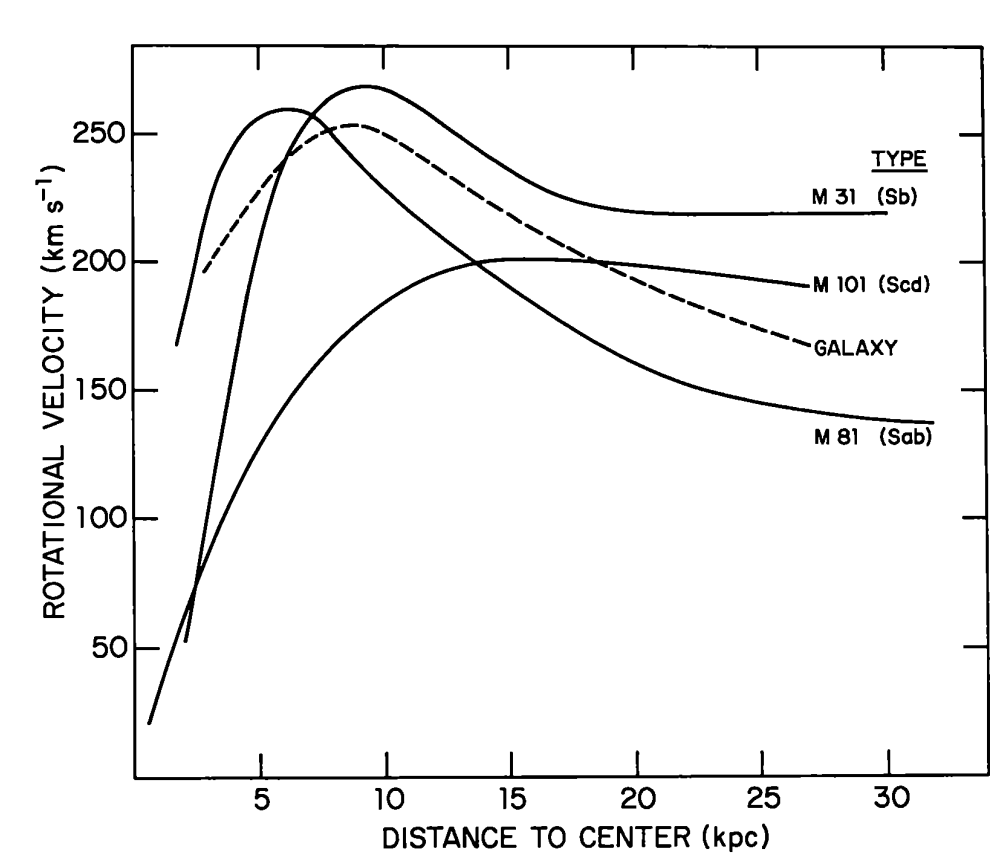
\includegraphics[width=0.6\linewidth]{graphs/rotation-curves}
	\caption{Rotation curves of various galaxies \cite{1973rotationcurves}, where the continuous lines represents the rotational velocity measured experimentally and the dashed one  represents the theoretical prediction.}
	\label{fig:rotation}
\end{figure}

As shown in \autoref{fig:rotation}, this is not the case, as $v$ is constant outside the galaxy's center, which indicates that $M \propto r$ outside the center.
This is one of the most compelling arguments for the existence of dark matter. 

\section{Dark Matter as a particle}

The term "dark matter"\ itself has undergone significant change during the previous few decades.
Today, this phrase is most usually used to refer to the particles that make up the majority of the matter density in our universe. Via the Cosmic Microwave Background (CMD), we can say that the current matter density of the universe is, $\Omega^0h^2\simeq0.13$, and the current baryonic matter density of the universe is, $\Omega^0h^2\simeq0.0225\pm0.00023$, baryonic matter is matter that makes up protons and neutrons \cite{2020}. By a simple subtraction we can calculate the non-baryonic matter density to be, $\Omega^0h^2\simeq0.11$, which allows us to see that most of the matter that makes up the universe aren't particles that constitute atoms, this non-baryonic matter is DM.

DM can be produced through: Freeze-in, Freeze-out, cosmic strings, domain walls and misalignment \cite{kolb}\cite{Marsh_2016}\cite{GONDOLO}\cite{Hall:2009bx}.

When looking at the DM problem through the perspective of the SM of particle physics, the three neutrinos stand out, as we notice that DM has characteristics very similar to neutrinos. The main properties of DM are its stability, neutrality, it only interacts with gravitational fields, and its cold, after the structure formation.
In contrast to every other known particle types, neutrinos are stable - or at least very long lived - and do not interact with electromagnetic or strong fields. These are some of the necessary properties for practically any viable candidate for dark matter\cite{STEIGMAN1985375}.
And even though we now know that dark matter in the form of neutrinos from the standard model would not be able to explain the observed large-scale structure of our Universe, these particles serve as a crucial model for an hypothetical class of particles, known as WIMPs, or weakly interacting massive particles. 
In this day and age, WIMPs are the strongest candidate for DM, but the lack of experimental evidence makes physicists lose interest in this candidate \cite{Moore_1999}\cite{10.1093/mnras/193.2.189}.

The main property of a given dark matter candidate, that numerical simulations can examine is whether it was relativistic (hot) or non-relativistic (cold) during the period of structure formation ($T\sim 10^5K$).

Lately, there has been a lot of interest focused on ultralight particles for DM candidates, with masses around $m\sim\mathcal{O}\left(10^{-10}-10^{-20}\right)\si{\eV}$,  
however these particles cannot be detected through direct detection experiments, but there have been developments in the area of gravitational waves that can uncover the truth about this hypothesis, which will be the main topic in this work.
\chapter{Ultralight Bosons}
\label{chapter:Ultralight Bosons}

\section{Introduction to particle physics}

Particle physics is an area of physics where it's studied the fundamental structure of the universe.  In this work, we are going to use natural units where $c=\hbar=1$, this is to simplify the calculations, and equations, as well use the term Lagrangian instead of Lagrangian density.

\subsection{Symmetries}
Particle physics revolves around the concept of symmetry and symmetry breaking, this concept is also important in mathematics in the area of Group theory.
Symmetry is a property of an object, that under a certain operation the object remains the same. We define those operations as a group.

\subsubsection{Continuous symmetries}
Certain symmetries are composed of continuous operations, for example, rotating a circle by an angle, it doesn't matter which angle we choose, the object suffers no change.

Noether's theorem says that \cite{Noether1918},
\textit{The invariance of the Lagrangian $\mathcal{L}$ under a continuous symmetry implies the existence of a conserved quantity.}

Taking into account the Noether's theorem, it's possible to verify:
\begin{itemize}
	\item Space-time symmetry:
	They result in energy-momentum conservation and are characterized by the Poincaré group. Inferred from this law as conserved quantities or charges are energy, linear momentum, and total angular momentum. 
	\item Internal symmetry:
	Is a symmetry acting on fields, these can be global, independent of the space-time point, and local, dependant on the space-time point, the latter  are known as gauge symmetries. Where the internal particle charges emerge, electric charge, hypercharge, weak spin or colour charge.
	The quantity usually conserved is current-density
\end{itemize}


\subsection{U(1) symmetry}

In this section, we are going to use the Klein-Gordon equation to prove the gauge symmetry, note that we can use the Dirac equation
\begin{equation}
	\label{KG}
	(\Box + m^2)\phi = 0\,,
\end{equation}
where $\phi$ is a scalar field \cite{grif} and $\Box=\left(\frac{\partial^2}{\partial t^2}-\nabla^2\right)$.

Let us consider the Klein-Gordon Lagrangian for a free complex scalar
\begin{equation}
	\label{lKG}
	\mathcal{L}_{KG}(\phi,\partial_\mu\phi)=K-V=g^{\mu\nu}\partial_\mu\phi^*\partial_\nu \phi - m^2 \phi^*\phi\,,
\end{equation}
where $K$ and $V$ are the kinetic and potential term, respectively, $\partial_\mu=\frac{\partial}{\partial x_\mu}=(\frac{\partial}{\partial t},-\vec{\nabla})$, and $g^{\mu\nu}=diag(+,-,-,-)$ is the Minkowski metric.
\subsubsection{Global symmetry}
Let's introduce the following global phase transformation
\begin{equation}
	\label{GPT}
	\phi\rightarrow \phi'=e^{-iq\alpha}\phi\,,
\end{equation}
where $\alpha$ is a global parameter, global as in it's equal at every space-time point, and $q$ 
represents the charge of the scalar field.

The Lagrangian in \autoref{lKG} gets transformed to
\begin{align}
	\label{tlKG}
	\begin{array}{lll}
			\mathcal{L}_{KG}(\phi',\partial_\mu\phi')&=g^{\mu\nu}\partial_\mu(e^{iq\alpha}\phi^*)\partial_\nu(e^{-iq\alpha}\phi) - m^2 (e^{iq\alpha}\phi^*)(e^{-iq\alpha}\phi) \\
			&=g^{\mu\nu}\partial_\mu\phi^*\partial^\nu \phi - m^2 \phi^*\phi \\
			&=\mathcal{L}_{KG}(\phi,\partial_\mu\phi)\,,
	\end{array}
\end{align}
and so we conclude that the Klein-Gordon Lagrangian remains invariant under a global phase transformation.
So we see that \autoref{GPT} is actually a unitary transformation of one dimension, and this class of groups are denoted as $U\textrm{(1)}$ symmetries. 

\subsubsection{Local symmetry}

Let us consider the same Lagrangian as in \autoref{lKG}, but now we replace the global parameter, with a local one, $\alpha(x^\mu)$, which depends on the space-time point defined by
\begin{equation}
	\phi \rightarrow \phi'=e^{-iq\alpha(x^\mu)}\phi\,
\end{equation}
we get
\begin{align}
	\begin{array}{lllll}
		\mathcal{L}_{KG}(\phi',\partial_\mu\phi')&=g^{\mu\nu}\partial_\mu(e^{iq\alpha(x^\mu)}\phi^*)\partial_\nu(e^{-iq\alpha(x^\mu)}\phi) - m^2 (e^{iq\alpha(x^\mu)}\phi^*)(e^{-iq\alpha(x^\mu)}\phi) \\
		&=g^{\mu\nu}(iq\partial_\mu\alpha(x^\mu)e^{iq\alpha(x^\mu)}\phi^*+e^{iq\alpha(x^\mu)}\partial_\mu\phi^*)\times \\ 
		&(-iq\partial_\nu\alpha(x^\mu)e^{-iq\alpha(x^\mu)}\phi+e^{-iq\alpha(x^\mu)}\partial_\nu\phi) - m^2\phi^*\phi \\
		&=\mathcal{L}_{KG}(\phi,\partial_\mu\phi)+q^2g^{\mu\nu}\partial_\nu\alpha(x^\mu)\partial_\nu\alpha(x^\mu)\phi^*\phi \\
		&-iqg^{\mu\nu}e^{iq\alpha(x^\mu)}\partial_\mu\phi^*\partial_\nu\alpha(x^\mu)\phi+iqg^{\mu\nu}e^{-iq\alpha(x^\mu)}\partial_\nu\phi\partial_\mu\alpha(x^\mu)\phi^*\,,
	\end{array}
\end{align}
therefore we see that the free Klein-Gordon theory is by no means $U\textrm{(1)}$ invariant.

Let's assume that gauge invariance is a fundamental law of the universe, the way we make our theory invariant is by redefining our partial derivative.
A gauge transformation is not expected to modify any observable values, observable quantities should not be directly dependent on the field's derivative.
Instead, we propose replacing the partial derivatives with the gauge covariant derivative 
\begin{equation}
	\label{pd1}
	\partial_\mu\rightarrow\mathcal{D}_\mu =\partial_\mu+V_\mu\,.
\end{equation}

The condition that guarantees the theory to be invariant is given by
\begin{equation}
	\label{invariancecondition}
	(\mathcal{D}_\mu \phi)'=e^{-iq\alpha(x)}\mathcal{D}_\mu \phi\,,
\end{equation}
using the \autoref{pd1} and \autoref{invariancecondition} we get
\begin{align}
	\begin{array}{ll}
		(\mathcal{D}_\mu \phi)'=(\partial_\mu+V_\mu')\phi'&=e^{-iq\alpha(x^\mu)}\left[\partial_\mu+V_\mu'-iq\partial_\mu\alpha(x^\mu)\right]\phi =e^{-iq\alpha(x^\mu)}\mathcal{D}_\mu \phi \\
		& \Leftrightarrow \mathcal{D}_\mu=\partial_\mu+V_\mu'-iq\partial_\mu\alpha(x^\mu)\,,
	\end{array}
\end{align}
and making $V_\mu=iqA_\mu$, where $A_\mu$ is a gauge field and using \autoref{pd1}, we can see that
\begin{equation}
	\label{gaugefieldchange}
	A_\mu'=A_\mu+\partial_\mu\alpha(x^\mu)\,,
\end{equation}
and so we can now define the covariant derivative, as
\begin{equation}
	\label{covdev}
	\mathcal{D}_\mu = \partial_\mu + iqA_\mu\,.
\end{equation}

Note that this gauge covariant derivative will remain unchanged whenever we apply a gauge transformation since the change in the partial derivative will now be balanced out by the change in the gauge field. The gauge covariant derivative can be explained intuitively as a means to alter the derivative operator so that the outcome is unaffected by a gauge transformation.
This is crucial since a gauge transformation is meant to restore the system to its initial condition while merely changing the arrangement of unobservable degrees of freedom.

Another approach is using the "kinetic"\ term in \autoref{lKG}, it relates to the field propagator and it defines how the particle moves in empty space.
The translation is generated by the derivative, and a finite translation is constructed by repeatedly applying infinitesimal translations.
The consequence is to create an infinitesimal phase change that goes along with each infinitesimal translation when the partial derivative is replaced by the gauge covariant derivative.
As a result, a phase shift is present along with a finite translation. 

\subsubsection{Spontaneous symmetry breaking}
The mechanism of SSB is one of the most potent concepts in current theoretical physics.
It serves as the foundation for the majority of recent advances in the statistical mechanics description of phase transitions as well as the description of collective events in solid state physics.
Additionally, it has made it possible to combine electromagnetic, weak, and strong interactions in elementary particle physics.
Philosophically, the concept is exceedingly complex and nuanced (which is partly why its successful application is a relatively recent accomplishment), and popular explanations of it fall short of doing it credit. 

The usual, cheap explanation for this phenomenon is that it results from the presence of an asymmetrical absolute minimum, or "ground state", which is shown in the \autoref{fig:SSB}, for the potential, $V(\phi)=\alpha |\phi|^2+\beta|\phi|^4$

\begin{figure}[H]
    \centering
	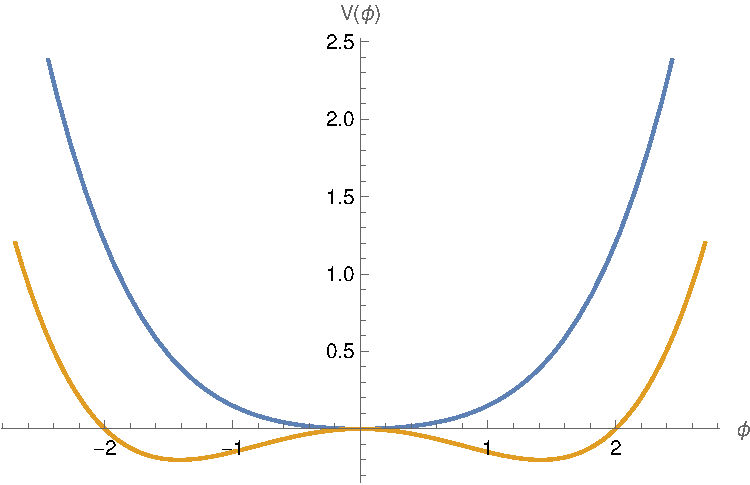
\includegraphics[width=0.7\linewidth]{graphs/SSB.pdf}
	\caption{Example of a Spontaneous symmetry breaking, with the blue line representing the symmetrial ground state ($\alpha>0$,$\beta>0$), and the orange line representing the asymmetrical ground state ($\alpha<0$,$\beta>0$).}
	\label{fig:SSB}
\end{figure}
\noindent This symmetry breaking occurs when we change the sign of the coupling terms of the interactions.

The main advantage of this symmetry breaking is due to the Goldstone theorem \cite{grif}, which says
\label{goldstone}

\textit{spontaneous breaking of a continuous
global symmetry is always accompanied by the appearance of one or more massless scalar
(spin-0) particles}.

\section{Bosonic sector}

In this section, we are going to take a quick look at the theory invariant under the symmetry $\textrm{SU}(2)_W \times  \textrm{U}(1)_Y$, denoted as ElectroWeak symmetry (EW) \cite{grif} \cite{Freitas_2021}.
Let the Higgs potential scalar be given by,
\begin{equation}
	V_0(H)=\mu_{H}^{2}H^{\dag}H+\frac{1}{2}\lambda_H(H^{\dag}H)^2\,,
\end{equation}
where $H$ is the Higgs field, a SU$(2)_W$ complex scalar doublet, and is written as
\begin{equation}
	H=\frac{1}{\sqrt{2}}
	\left(\begin{array}{c} w_1+iw_2 \\ v_h+h+iz \end{array} \right)\,,
\end{equation}
where $v_h$ is the vacuum expectation value VEV which describes the classical ground state of the theory, $v_h\simeq$ \SI{246}{G\eV}, $h$ represents the radial fluctuations. When a SSB occurs, due to the Higgs doublet 
\begin{equation}
	\langle H \rangle = \frac{1}{\sqrt{2}}\left(
	\begin{array}{c}
	0 \\
	v_h
	\end{array}\right)\,
\end{equation}
the goldstone modes $w_{1,2}$, that appear due to the Goldstone Theorem \ref{goldstone}, and z are absorved by the longitudinal degrees of freedom of the $W^{\pm}$ and $Z$ gauge bosons.

The kinetic term of the Lagrangian, between the coupling of EW vector bosons with the Higgs doublet, is
\begin{equation}
	\mathcal{L}_{kin}\supset(\mathcal{D}_\mu H^\dag) (\mathcal{D}^\mu H)\,,
\end{equation}
where $D_\mu$ is the covariant derivative, which is defined by
$\mathcal{D}_\mu=\partial_\mu+ig_1\frac{\sigma_a}{2}A_\mu^a+ig_2YB_\mu 
$, $g_{1,2}$ are the U$(1)_Y$ and SU$(2)_W$ gauge couplings, $Y$ is the hypercharge, $\sigma_a$ ($a$ = x,y,z) are the Pauli matrices, and the $B_\mu$, $A_\mu^a$ the massless EW gauge bosons.

\section{Ultralight complex scalar}
This section serves as a simple example of how we can obtain an ultralight particle.
The model in question will contain an additional complex singlet $\phi$ charged under a global U$(1)_G$ symmetry, such that it is invariant under the global phase transformation, $\alpha$, \cite{Freitas_2021}
\begin{equation}
	\phi \rightarrow e^{i\alpha}\phi\,.
\end{equation}

The potential under this new complex singlet, before the electroweak symmetry breaking (EWSB), is defined as
\begin{equation}
	\label{potential}
	V(H,\phi)=V_0(H)+ \mu_\phi^2\phi^*\phi+\frac{1}{2}\lambda_\phi|\phi^*\phi|^2+\lambda_{H\phi}H^{\dag}H\phi^*\phi\,,
\end{equation}
where $\lambda_{H\phi}$, is commonly known as the Higgs portal coupling, the coupling term between the boson scalar and the Higgs doublet.

The conditions which allow us to have a SSB are
\begin{equation}
	\label{couplingtermconditions}
	\lambda_H,\lambda_\phi>0 \quad \textrm{and} \quad \lambda_H\lambda_\phi-\lambda_{H\phi}^2>0\,,    
\end{equation}
they allow us to write $\mu_H^2=-\lambda_Hv_h^2$, this $\mu_H^2$ appears as a consequence of the minimum of the potential, and the Hessian matrix of \autoref{potential} and replacing $\mu_H^2$, this matrix contains the mass terms and reads as \cite{Freitas_2021}
\begin{equation}
	M^2=\left( \begin{array}{cccc} 
		0_{3\times3} & 0_{3\times1} & 0_{3\times1} & 0_{3\times1} \\
		0_{1\times3} & 2\lambda_Hv_h^2 & 0 & 0 \\
		0_{1\times3} & 0 & \mu_\phi^2+\frac{1}{2}\lambda_{H\phi}v_h^2 & 0 \\
		0_{1\times3} & 0 & 0 & \mu_\phi^2+\frac{1}{2}\lambda_{H\phi}v_h^2
	\end{array}\right)\,.
\end{equation} 

This matrix is already in the diagonal form so it's not needed to be diagonalized and so we can see that there is a Goldstone boson, the masses of the SM-Higgs boson and 2 new complex scalar particles are given by
\begin{equation}
	m_h^2=2\lambda_Hv_h^2 \quad \quad \quad m_\phi^2=\mu_\phi^2+\frac{1}{2}\lambda_{H\phi}v_h^2\,.
\end{equation}
The relevant interactions with the singlet $\phi$ are given by
\begin{equation}
	\lambda_{h\phi\phi}=v_h\lambda_{H\phi}\,, \quad \quad
	\lambda_{hh\phi\phi}=\lambda_{H\phi}\,, \quad \quad
	\lambda_{\phi\phi\phi\phi}=\lambda_\phi\,.
\end{equation}

This model can allow an ultralight complex scalar, it can be obtain via a feebly interacting scenario, which consists of making the portal coupling very small, $10^{-42}\gtrsim \lambda_{H\phi} \gtrsim 10^{-62}$, and so the mass of our complex scalar $\phi$ gets around, $10^{-10}\gtrsim m_{\phi} \gtrsim 10^{-20}$ \si{\eV} \cite{Freitas_2021}.

\section{Real pseudo-Goldstone Boson}

In the previous section, we took a look at complex scalars (and their advantages). However real scalars also have quite a bunch of interesting advantages. 
Let's begin by considering the same potential as in \autoref{potential}, and that not only the Higgs doublet develops a VEV but also the $\phi$ scalar, $v_\sigma$. But now that we break the U$(1)_G$ symmetry, due to Goldstone's theorem, a new massless real scalar emerges in the physical particle spectrum.
However evidence shows that this isn't enough to get anywhere, so let us take a look at the introduction of a small soft symmetry breaking such that \cite{Freitas_2021}
\begin{equation}
	\label{vsoft}
	V(H,\phi)\rightarrow V(H,\phi)+V_{soft}\,, \quad \quad \textrm{where} \quad \quad V_{soft}=\frac{\mu_s^2}{2}(\phi^2+\phi^{*2})\,,
\end{equation}    
the $V_{\textrm{soft}}$ scalar potential is used as an explicit symmetry breaking, and it occurs when we introduce an external term in our theory which will turn our theory invariant, this will helps us to give mass to our Goldstone boson, from the SSB, and we call this new Golstone Boson, pNGB.

The Goldstone mode can be described as a phase, $\theta$, and so the $\phi$ scalar can be expressed as
\begin{equation}
	\phi=\frac{1}{\sqrt{2}}(\sigma+v_\sigma)e^{i\theta/v_\sigma}\,,
\end{equation}
with $\sigma$ denoting quantum fluctuations in the radial directions around the classical field, $v_\sigma$. And so our $V_\textrm{soft}$ scalar potential in \autoref{vsoft} can be written as 
\begin{equation}
	\label{newvsoft}
	V_\textrm{soft}=\dfrac{\mu_s^2}{2}(\sigma+v_\sigma)^2\cos\left(\dfrac{2\theta}{v_\sigma}\right)\,.
\end{equation}


Thus our degrees of freedom are $\sigma$, $h$, and $\theta$, and so let's determine the minimization conditions taking
\begin{equation}
	\frac{\partial V}{\partial \sigma}=\frac{\partial V}{\partial h}=\frac{\partial V}{\partial \theta}=0 \Leftrightarrow \left\{\begin{array}{c}
		\mu_H^2=-\frac{1}{2}(v_h^2\lambda_H+v_\sigma^2\lambda_{H\phi}) \\
		\mu_\phi^2=-\frac{1}{2}(v_\sigma^2\lambda_\phi+v_h^2\lambda_{H\phi}+2\mu_s^2)
	\end{array} \right. \,,
\end{equation}
where $\theta=n\pi v_\sigma \textrm{ and } h=\sigma=0$.

The corresponding Hessian matrix is defined by
\begin{equation}
	M^2=\left(\begin{array}{ccc}
		\dfrac{\partial^2V}{\partial h^2} & \dfrac{\partial^2V}{\partial h \partial\sigma} & \dfrac{\partial^2V}{\partial h \partial\theta} \\ [8pt]
		\dfrac{\partial^2V}{\partial \sigma \partial h} & \dfrac{\partial^2V}{\partial \sigma^2} & \dfrac{\partial^2V}{\partial \sigma \partial\theta} \\ [8pt]
		\dfrac{\partial^2V}{\partial \theta \partial h} & \dfrac{\partial^2V}{\partial \theta \partial\sigma} & \dfrac{\partial^2V}{\partial\theta^2}
	\end{array}\right)=\left(\begin{array}{ccc}
		v_h^2\lambda_H & v_hv_\sigma\lambda_{H\phi} & 0 \\
		v_hv_\sigma\lambda_{H\phi} & v_\sigma^2\lambda_\phi & 0 \\
		0 & 0 & -2\mu_s^2\,,
	\end{array}\right)
\end{equation}
notice that the matrix isn't diagonalized, so let's rotate the matrix to the physical basis, where we can more easily see the physical particle spectrum, we obtain
\begin{equation}
	m^2=U^\dag M^2 U = \left(\begin{array}{ccc}
		m^2_{h_1} & 0 & 0 \\
		0 & m^2_{h_2} & 0 \\
		0 & 0 & m^2_{\theta}
	\end{array}\right)\,,
\end{equation}
where the eigenvalues are
\begin{equation}
\label{masses}
	\begin{array}{c}
		m^2_{h_{1,2}}=\frac{1}{2}\left[v_h^2\lambda_H+v_\sigma^2\lambda_\phi\mp\sqrt{v_h^4\lambda_H^2+v_\sigma^4\lambda_\phi^2+2v_h^2v_\sigma^2(2\lambda_{H\phi}^2-\lambda_H\lambda_\phi)}\right] \\ 
		m^2_\theta=-2\mu_s^2\,,
	\end{array}
\end{equation}
where $U$ is the matrix containing the eigenvectors, which can be expressed as a matrix rotation and reads as
\begin{equation}
	U=\left(\begin{array}{lll}
		\cos(\alpha) & \sin(\alpha) & 0 \\
		-\sin(\alpha) & \cos(\alpha) & 0 \\
		0 & 0 & 1
	\end{array}\right)\,,
\end{equation}
where $\alpha$, is the mixing angle.
The physical basis vectors $h_1$ and $h_2$ can be represented in terms of the gauge eigenbasis ones $h$ and $\sigma$, as follows
\begin{equation}
\label{mixing}
	\left(\begin{array}{l}
		h_1 \\
		h_2 \\
		\theta 
	\end{array}\right)=U\left(\begin{array}{l}
	h \\
	\sigma \\
	\theta 
\end{array}\right)\Leftrightarrow \left\{\begin{array}{cc}
     h=\cos(\alpha)h_1-\sin(\alpha)h_2 \\
     \sigma=\sin(\alpha)h_1+\cos(\alpha)h_2 
\end{array}\right.\,,
\end{equation}

When expanding the "kinetic"\ term of the scalar field, we get
\begin{equation}
    \partial_\mu\phi^*\partial^\mu\phi=\dfrac{1}{2}\left[(\partial\sigma)^2+(\partial\theta)^2\dfrac{(\sigma+v_\sigma)^2}{v_\sigma^2}\right]\,,
\end{equation}
we are able to notice that there is the appearing of cubic interacting between $\sigma\theta\theta$ from $(\partial\theta)^2\sigma$, using $\autoref{mixing}$, it reads as
\begin{equation}
\label{sigmathetatheta}
    (\partial\theta)^2\sigma=-\dfrac{1}{2}\left[\sin(\alpha)m_{h_1}^2h_1+\cos(\alpha)m_{h_2}^2h_2\right]\theta^2+\sigma m_\theta^2\theta^2\,.
\end{equation}

Notice that in \autoref{newvsoft} expanding the cosine with a Taylor series, $\cos(x)\simeq 1-\dfrac{x^2}{2}$, will get us
\begin{equation}
\label{taylorcosine}
	\cos\left(\dfrac{2\theta}{v_\sigma}\right)\simeq 1 - \dfrac{2\theta^2}{v_\sigma}\,,
\end{equation}
this also means that the theory is invariant under a $Z_2 \in U\textrm{(1)}_G$ symmetry where the pNGB transforms as $\theta \rightarrow -\theta$.
With this new expansion we can see that the soft breaking potential, in \autoref{newvsoft}, forms a cubic coupling term $\dfrac{m_\theta^2}{v_\sigma^2}\sigma\theta^2$, which will cancel out with the last term from \autoref{sigmathetatheta}.

Note that the mixture of $h$ and $\sigma$, allows for the appearance of a partial width decay of the Higgs like particles, $h_1$ or $h_2$, into $\theta\theta$, in \autoref{sigmathetatheta}, being $\Gamma(h_i\rightarrow\theta\theta)\propto U_{1i}^2/v_\sigma^2$, the initial constraint for the mixing angle, backed up by experiments, is $|\sin(\alpha)| < 0.3$ \cite{robens2021extended}, and as the value of $|\sin(\alpha)|$ decreases, the probability of $h_1$ decaying into $\theta\theta$ decreases as well, but the probability of $h_2$ decaying into $\theta\theta$ increases. Later in this work this will become relevant.

This approach provides three real scalars.
First, one of the Higgs bosons, either $h_1$ or $h_2$, must be the SM-like Higgs, whereas the other can be heavier or lighter than \SI{125}{G\eV}.
Second, the pNGB $\theta$ derives its mass from a soft-breaking parameter and is a candidate for a real scalar with an ultralight mass. Its mass comes from a minor violation of the global $U\textrm{(1)}_G$ symmetry\cite{Freitas_2021}. 

The expansion in \autoref{taylorcosine} allows us to see the appearance of interactions with $\theta$, and the cubic and quartic coupling terms of these interactions are \cite{Freitas_2021}
\begin{align}
	\label{couplingterms}
	\begin{array}{lll}
	&\lambda_{\theta\theta h_i}=\dfrac{m_{h_1}^2}{v_\sigma}U_{2i}\,,\\	[8pt]
	&\lambda_{\theta\theta h_i h_j}=\dfrac{1}{4}\left[\lambda_\phi U_{2i}U_{2j}+(-1)^{i+j}\lambda_{H\phi}U_{1i}U_{1j}\right]\,,\\ [8pt]
	&\lambda_{h_i SM SM}=U_{1i}g_{SM}\,.
	\end{array}
\end{align}

In terms of these parameters, the quartic terms can be stated as follows
\begin{align}
 \label{couplingtermsfrominteraction}
 \begin{array}{lll}
 	&\lambda_{H\phi}=\dfrac{\sin(2\alpha)(m_{h_1}^2-m_{h_2}^2)}{2v_\sigma v_h}\,, \\[8pt]	
 	&\lambda_{\phi}=\dfrac{\cos^2(\alpha)m_ {h_2}^2+\sin^2(\alpha)m_{h_1}^2}{v_\sigma^2}\,, \\[8pt]
 	&\lambda_{H}=\dfrac{\cos^2(\alpha)m_ {h_1}^2+\sin^2(\alpha)m_{h_2}^2}{v_h^2}\,.
 \end{array}
\end{align}
And the quartic self-interaction of the pNGB is
\begin{equation}
	\lambda_{\theta\theta\theta\theta}=-\dfrac{m_\theta^2}{6v_\sigma^2}\,.
\end{equation}

Note that $\lambda_{H\phi}$ has to be small due to the radiative corrections, this is not the main topic of this work, for more information on the subject check \cite{Freitas_2021}.
\chapter{Thermodynamics of the expanding universe}
\label{chapter:thermodynamicsofearlyuniverse}

In this chapter, our objective is to understand the evolution of the early universe, so we will make a brief review of the thermodynamics in the equilibrium of the early universe, following \cite{kolb}.

We are able to predict how the universe behaved due to the Cosmic Microwave Background (CMB) being approximately equal to the spectra of a black body, so we assume that in the primordial universe the particles from the SM are in equilibrium.

\section{Thermodynamics in equilibrium}
The number density, $n$, energy density, $\rho$, and the pressure, $P$ of a gas of particles with a degree of freedom, $g$, distinguish the thermodynamic properties of the gas and are defined as a function of the distribution function $f(\vec{p},t)$:
\begin{equation}
	\label{eqn:3.1}
	n(t)\equiv\frac{g}{(2\pi)^3}\int f(\vec{p},t) d\vec{p}\,,
\end{equation}
\begin{equation}
	\label{eqn:3.2}
	\rho(t)\equiv\frac{g}{(2\pi)^3}\int E(\vec{p})f(\vec{p},t) d\vec{p}\,,
\end{equation} 
\begin{equation}
	\label{eqn:3.3}
	P(t)\equiv\frac{g}{(2\pi)^3}\int \frac{p^2}{3E}f(\vec{p},t) d\vec{p}\,,
\end{equation}  
where $\vec{p}=(p_x,p_y,p_z)$, $d\vec{p}\equiv dp_xdp_ydp_z$ and E=$\sqrt{p^2+m^2}$. The phase pace equilibrium distribution function for a particle $i$ will be given by one of the three following distributions
\begin{equation}
	f_i^{eq} = \left\{ 
	\begin{array}{lll}
		\frac{1}{e^{(E_i-\mu_i)/T}+1}\,, \quad\textrm{Fermi-Dirac}\,,\\
		\frac{1}{e^{(E_i-\mu_i)/T}-1}\,, \quad\textrm{Bose-Einstein}\,,\\
		e^{-(E_i-\mu_i)/T}\,, \quad \textrm{Maxwell-Boltzmann}\,,	
	\end{array}
	\right.
\end{equation}
where $E_i$ and $\mu_i$ is the energy and chemical potential of the particle $i$, respectively. The Fermi-Dirac (Bose-Einstein) statistic refers to particles with half-integer (integer) spin.

Using spherical symmetry we can simplify, $d\vec{p}=4\pi p^2dp,$ we can now rewrite the Equations (\ref{eqn:3.1}), (\ref{eqn:3.2}) and (\ref{eqn:3.3}) in function of the energy, $E$, given as
\begin{equation}
	\label{eqn:3.5}
	n_R=\frac{g}{2\pi^2}\int_{m}^{\infty} \frac{(E^2-m^2)^{1/2}}{e^{(E-\mu)/T}\pm 1}dE\,,
\end{equation}
\begin{equation}
	\label{eqn:3.6}
	\rho_R=\frac{g}{2\pi^2}\int_{m}^{\infty} \frac{(E^2-m^2)^{1/2}}{e^{(E-\mu)/T}\pm 1}E^2dE\,,
\end{equation} 
\begin{equation}
	\label{eqn:3.7}
	P_R=\frac{g}{6\pi^2}\int_{m}^{\infty} \frac{(E^2-m^2)^{3/2}}{e^{(E-\mu)/T}\pm 1}dE\,,
\end{equation}
where "R"\ refers to radiation, the inferior limit of the integral refers to the lowest energy a particle can have, which is its mass, $m$.

Let's take a look at a generalized solution for the Fermi-Dirac and Bose-Einstein distributions, when we take into account that the mass of the particle is so low such that, $m \simeq 0$, we get
\begin{equation}
	\nonumber
	\int_{m}^{\infty} \frac{(E^2-m^2)^s}{e^{(E-\mu)/T}\pm 1}dE =  	\int_{0}^{\infty}\frac{E^s}{e^{\frac{E-\mu_i}{T}}\pm 1}dE\,,
\end{equation}
by making $k=\frac{E}{T}$ and $\mu=\frac{\mu_i}{T}$, we get \cite{fermi}\cite{bose}
\begin{equation}
	\label{eqn:3.8}
	\int_{0}^{\infty}\frac{E^s}{e^{\frac{E-\mu_i}{T}}\pm 1}dE =\int_{0}^{\infty}\frac{(Tk)^s}{e^{k-\mu}\pm 1}Tdk=T^{s+1}\int_{0}^{\infty}\frac{k^s}{e^{k-\mu}\pm 1}dk=\mp T^{s+1} \Gamma(s+1)Li_{1+s}(\mp e^\mu)\,,
\end{equation}
where the polylogarithm or Jonquière's function and the Gamma function, are respectively defined by \cite{poly}
\begin{equation}
	\label{eqn:3.9}
	Li_n(z)\equiv\sum\limits_{k=1}^\infty \frac{z^k}{k^n} \quad \textrm{and} \quad \Gamma(s+1)=\int_{0}^{\infty} e^{-x}x^s dx=s!\,.
\end{equation}

At the ultra-relativistic limit (radiation), $T\gg m,\mu_i$. We can simplify $\mu=\mu_i/T \simeq 0$ and so the polylogarithm function in \autoref{eqn:3.8} can be simplified into
\begin{equation}
	\label{eqn:3.10}
	Li_{s+1}(\mp 1)=\sum\limits_{k=1}^{\infty}\frac{(\mp1)^k}{k^{s+1}}\,,
\end{equation}
now if we take a look at the solution of the following sum
\begin{equation}
	\label{eqn:3.11}
	\sum\limits_{k=1}^{\infty}\frac{(-1)^{k+1}}{k^s}=(1-2^{-s})\zeta(s+1)\,,
\end{equation}
where $\zeta(s)$ the Riemann zeta function, defined by
\begin{equation}
	\label{eqn:3.12}
	\zeta(s)=\sum\limits_{k=1}^{\infty}\frac{1}{k^s}\,,
\end{equation}
using the solutions in Equations (\ref{eqn:3.11}) and (\ref{eqn:3.12}) the generalized solution for ultra-relativistic particles, in \autoref{eqn:3.8}, gets reduced to 
\begin{equation}
	\int_{0}^{\infty}\frac{E^s}{e^{\frac{E-\mu_i}{T}}\pm 1}dE=\left\{ \begin{array}{c}
		T^{s+1}(1-2^{-s})\zeta(s+1)s!\,, \quad \textrm{Fermi-Dirac}\,, \\
		T^{s+1}\zeta(s+1)s!\,, \quad \textrm{Bose-Einstein}\,,	
	\end{array}\right.\,.
\end{equation}
Now we can easily integrate the Equations (\ref{eqn:3.5}), (\ref{eqn:3.6}) and (\ref{eqn:3.7}), knowing that $\zeta(4)=\pi^4/90$ to
\begin{equation}
	\label{eqn:3.14}
	n_{\textrm{R}}=\frac{g}{2\pi^2}\int_{0}^{\infty} \frac{E}{e^{E/T}\pm1}dE=\frac{g}{\pi^2}T^3\zeta(3)\left\{ \begin{array}{c}
		3/4\,, \quad \textrm{Fermi-Dirac}\,, \\
		1\,, \quad \textrm{Bose-Einstein}\,,
	\end{array}\right.
\end{equation}
\begin{equation}
	\label{eqn:3.15}
	\rho_{\textrm{R}}=\frac{g}{2\pi^2}\int_{0}^{\infty} \frac{E^3}{e^{E/T}\pm1}dE=g\frac{\pi^2}{30}T^4\left\{ \begin{array}{c}
		7/8\,,\quad \textrm{Fermi-Dirac}\,, \\
		1\,, \quad \textrm{Bose-Einstein}\,,
	\end{array}\right.
\end{equation} 
\begin{equation}
	\label{eqn:3.16}
	P_{\textrm{R}}=\frac{g}{6\pi^2}\int_{0}^{\infty} \frac{E^3}{e^{E/T}\pm1}dE=\frac{1}{3}\rho_{\textrm{R}}\,,
\end{equation}  
where the + and - refers respectively to the Fermi-Dirac and Bose-Einstein distributions.

Now let's take a look at the non-relativistic limit (matter), $T \ll m,\mu$, which follows the Maxwell-Boltzmann distribution, we can rewrite the Equations (\ref{eqn:3.1}), (\ref{eqn:3.2}) and (\ref{eqn:3.3}) in function of the momentum, $p$, given as

\begin{equation}
	\label{eqn:3.17}
	n_{\textrm{M}}\equiv\frac{g}{(2\pi)^3}\int e^{-\frac{(E-\mu)}{T}} d\vec{p}\,,
\end{equation}
\begin{equation}
	\label{eqn:3.18}
	\rho_{\textrm{M}}\equiv\frac{g}{(2\pi)^3}\int E(\vec{p})e^{-\frac{(E-\mu)}{T}} d\vec{p}\,,
\end{equation} 
\begin{equation}
	\label{eqn:3.19}
	P_{\textrm{M}}\equiv\frac{g}{(2\pi)^3}\int \frac{p^2}{3E}e^{-\frac{(E-\mu)}{T}} d\vec{p}\,,
\end{equation}  
where the subscript "M"\ means Matter (non-relativistic limit).

Let's take a look at a generalized solution to a certain integral, where we use spherical coordinates, $d\vec{p}=4\pi p^2 dp$
\begin{equation}
\label{eqn:3.20}
	\int p^k E^s e^{-\frac{(E-\mu)}{T}} d\vec{p}=4\pi e^{\mu/T}T^s\int_{0}^{\infty} p^{k+2} \frac{(p^2+m^2)^{s/2}}{T^s} e^{-\frac{\sqrt{p^2+m^2}}{T}} dp\,,
\end{equation}
substituting $x=\frac{p}{T}$ and $\gamma=\frac{\mu}{T}$, in \autoref{eqn:3.20}
\begin{equation}
	\label{eqn:3.21}
	4\pi e^{\mu/T}T^{s+k+3}\int_{0}^{\infty} x^{k+2}(x^2+\gamma^2)^{s/2}e^{-\sqrt{x^2+\gamma^2}} dx\,,
\end{equation}
by taking into account $T \ll m,\mu$, we can do the following approximation to simplify the integration
\begin{equation}
\label{eqn:3.22}
	(x^2+\gamma^2)^{s/2}=\gamma^s\left[1+\left(\frac{x}{\gamma}\right)\right]^{s/2} \approx \gamma^s+\frac{s}{2}\gamma^{s-2}x^2\,,
\end{equation}
then using Eq.(\ref{eqn:3.22}), the \autoref{eqn:3.21} becomes
\begin{equation}
	\label{eqn:3.23}
	4\pi e^{\mu/T}T^{s+k+3}\gamma^se^{-\gamma}\left[ \int_{0}^{\infty} x^{k+2}e^{-\frac{x^2}{2\gamma}}dx+\frac{s}{2}\gamma^{-2}\int_{0}^{\infty} x^{k+4}e^{-\frac{x^2}{2\gamma}}dx\right]\,,
\end{equation}
from Eq.(\ref{eqn:3.23}), $u=\frac{x^2}{2\gamma}$,
\begin{equation}
	4\pi e^{\mu/T}T^{s+k+3}\gamma^{s+1}e^{-\gamma}\left[(2\gamma)^{\frac{k+1}{2}}\int_{0}^{\infty} u^{(k+1)/2}e^{-u}du+\frac{s}{2}\gamma^{-2}(2\gamma)^{\frac{k+3}{2}}\int_{0}^{\infty} u^{(k+3)/2}e^{-u}du\right]\,,
\end{equation}
using the Gamma function, as shown in \autoref{eqn:3.9}, the \autoref{eqn:3.20}) becomes

\begin{equation}
	\label{eqn:3.24}
	4\pi T^{s+k+3}e^{-\frac{(m-\mu)}{T}} 2^{(k+1)/2} \left( \frac{m}{T}\right)^{\frac{k+3}{2}+s}
	\left[\left((k+1)/2\right)!+\frac{s}{2}\left(\frac{m}{T}\right)^{-1}\left((k+3)/2\right)!\right]\,.
\end{equation}

We can now determine the Equations (\ref{eqn:3.17}), (\ref{eqn:3.18}) and (\ref{eqn:3.19}), and so we get these solutions, knowing that $(1/2)!=\sqrt{\pi}/2$,
\begin{equation}
	\label{nM}
	n_{\textrm{M}}=\frac{g}{(2\pi)^3}\int e^{-\frac{(E-\mu)}{T}} d\vec{p}=g\left( \frac{mT}{2\pi}\right)^{\frac{3}{2}}e^{-\frac{(m-\mu)}{T}}\,,
\end{equation}
\begin{equation}
	\label{rhoM}
	\rho_{\textrm{M}}=\frac{g}{(2\pi)^3}\int E(\vec{p})e^{-\frac{(E-\mu)}{T}} d\vec{p}=n_{M}m\left[1+\frac{3}{2}\left(\frac{T}{m}\right)\right]\,,
\end{equation} 
\begin{equation}
	\label{PM}
	P_{\textrm{M}}=\frac{g}{(2\pi)^3}\int \frac{p^2}{3E}e^{-\frac{(E-\mu)}{T}} d\vec{p}=n_{M} 
	T\left[1-\frac{5}{6}\left(\frac{T}{m}\right)\right]\,.
\end{equation}


Assuming a period when $T \sim$ \SI{300}{G\eV}, and so during this time we can easily notice that $T\gg m,\mu$ and so the total energy density is equal to the sum of the energy density for each relativistic specie
\begin{equation}
	\rho_{\textrm{Total}}=\sum\limits_{i} \rho_\textrm{R}^{(i)}\,,
\end{equation}
where $i$ represents particles of the SM.

As the universe expands, its temperature decreases and so some particles become non-relativistic, behave accordingly to the Maxwell Boltzmann distribution, when $T \sim m$, and so the energy density of matter increases, so we can represent the energy density of the universe as
\begin{equation}
	\rho_{\textrm{Total}}=\sum\limits_{i}\rho_{\textrm{R}}^{(i)}+\sum\limits_{j}\rho_{\textrm{M}}^{(j)}\,,
\end{equation}
where $i$ and $j$ represent relativistic and non-relativistic particles, respectively.

Although some particles become non-relativistic as the temperature decreases, their contribution becomes negligible because their energy density, $\rho_{\textrm{M}}$, decreases exponentially as shown in Eq.(\ref{rhoM}), and so we can approximate the energy density in the primordial universe to
\begin{equation}
	\rho_{\textrm{Total}}\simeq\sum\limits_{i}\rho_{\textrm{R}}^{(i)}\,.
\end{equation}

Taking into account that species of particles can evolve with different temperatures, even in equilibrium, we can write the $\rho_{\textrm{R}}$ in terms of the temperature of photons, $T$, as follows

\begin{equation}
\label{3.32}
	\rho_{\textrm{R}}=\sum\limits_{b}\rho_{b}+\sum\limits_{f}\rho_{f}=\frac{\pi^2}{30}T^4g_*(T)\,,
\end{equation}
where, "b"\ stands for bosons, "f"\ stands for fermions, and $g_*(T)$ is
\begin{equation}
	g_*(T)=\sum\limits_{b}g_b\left(\frac{T_b}{T}\right)^4+\dfrac{7}{8}\sum\limits_{f}g_f\left(\frac{T_f}{T}\right)^4\,,
\end{equation}
putting away the photon and neutrinos we can write this as
\begin{equation}
	\nonumber
	\rho_{\textrm{R}}=\frac{\pi^2}{30}T^4\left[g_\gamma+\frac{7}{8}\sum\limits_{\nu}g_\nu\left(\frac{T_\nu}{T}\right)^4+\sum\limits_{b}g_b\left(\frac{T_b}{T}\right)^4+\frac{7}{8}\sum\limits_{f}g_f\left(\frac{T_f}{T}\right)^4\right]=
\end{equation}
\begin{equation}
	\nonumber
	=\rho_\gamma\left[1+\frac{1}{g_\gamma}\frac{7}{8}\left(\frac{T_\nu}{T}\right)^4\left(\sum\limits_{\nu}g_\nu+\sum\limits_{b}g_b\left(\frac{T_b}{T_\nu}\right)^4+\sum\limits_{f}g_f\left(\frac{T_f}{T_\nu}\right)^4\right)\right]\,,
\end{equation}
where $\rho_\gamma$ is
\begin{equation}
	\rho_\gamma=\frac{\pi^2}{30}T^4g_\gamma\,,
\end{equation}
and finally, we get
\begin{equation}
	\rho_{\textrm{R}}=\rho_\gamma\left[1+\frac{7}{8}\left(\frac{T_\nu}{T}\right)^4N_\textrm{eff}\right]\,,
\end{equation}
where $N_\textrm{eff}$ is the effective number of ultra-relativistic species ignoring the photon, and $g_\gamma=2$, as is given by
\begin{equation}
	N_\textrm{eff}=\frac{1}{g_\gamma}\left(\sum\limits_{\nu}g_\nu+\sum\limits_{b}g_b\left(\frac{T_b}{T_\nu}\right)^4+\sum\limits_{f}g_f\left(\frac{T_f}{T_\nu}\right)^4\right)\,,
\end{equation}
experiments using the CMB determine $N_\textrm{eff}=2.99 \pm 0.14$\cite{2020}.


\section{Collision Operator}
In the early universe, its contents were for the most part in thermal equilibrium, so it's a good approximation of making it in equilibrium, following \cite{kolb}.

The Boltzmann equation which describes the microscopic evolution of a particle's phase space distribution function $f(p^\mu,x^\mu)$, is given by:
\begin{equation}
	\hat{L}[f]=C[f]\,,
\end{equation}
where $\hat{L}$ is the Liouville operator and $C$ is the collision operator.


The collision operator for a process of annihilation while focusing on the particle 1 ($1 + 2 \Leftrightarrow 3 + 4$) is given by
\begin{align}
	\label{eqn:3.38}
	\begin{array}{lll}
		\dfrac{g}{(2\pi)^3}\mathlarger{\int} C[f_1]\dfrac{d^3p_1}{E_1}
		&=\pm \mathlarger{\int} (2\pi)^4 \delta^4(\mathcal{P}_1 + \mathcal{P}_2 - \mathcal{P}_3 - \mathcal{P}_4)\\[15pt]
		&\times[|\overline{M}|^2_{1 + 2 \rightarrow 3 + 4}f_1 f_2 (1\pm f_3)(1\pm f_4) \\ [15pt]
		&-|\overline{M}|^2_{3 + 4 \rightarrow 1 + 2}f_3 f_4 (1\pm f_1)(1\pm f_2) ] d\Pi_1 d\Pi_2 d\Pi_3 d\Pi_4\,,
	\end{array}
\end{align}
where $\mathcal{P}_i=(E_i,\vec{p}_i)$, $d\Pi_i=\dfrac{g_i d\vec{p}_i}{2(2\pi)^3E_i}$, the $\pm$ refers to which direction the process takes, where + refers to the production of the particle 1 ($3+4\rightarrow1+2$) and - refers to it's consumption ($1+2\rightarrow 3+4$), in the term $(1\pm f_i)$, the + appears when $i$ is a boson and - when it's a fermion, and $|\overline{M}|^2$ is the mean of initial and final spins squared.
In order to simplify we are going to assume
\begin{equation}
	|\overline{M}|^2 \equiv |\overline{M}|^2_{1+2\rightarrow 3+4} \equiv |\overline{M}|^2_{3+4\rightarrow 1+2} \,,
\end{equation}
this assumption is well explained in \cite{kolb}.

The amplitude is defined as
\begin{equation}
	|\overline{M}|^2=\frac{S_{12}S_{34}}{g_1g_2g_3g_4}|M|^2\,,
\end{equation} 
where $|M|^2$ is the amplitude squared of the processes, and the symmetrization factor $S_{i,j}=1/n_{i,j}!$ which accounts for identical particles, if the particles $i$ and $j$ are the same, $S_{i,j}=0.5$ and if they are different $S_{i,j}=1$ (note that even particles and anti-particles are different particles). 
If we assume that the particle $i$ is in thermal equilibrium, we have that $E_i>T$ so we can approximate the term $1 \pm f_i \simeq 1$, as the particle $i$ will behave according to the Maxwell-Boltzmann distribution, as shown in \autoref{fig:1-fi}.

\begin{figure}[H]
	\centering
	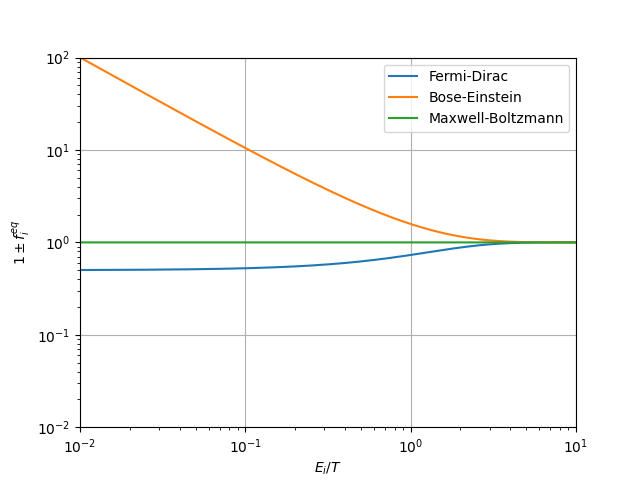
\includegraphics[width=0.7\linewidth]{graphs/1+-fi}
	\caption{Dependance of $1\pm f_i$ with $E_i/T$.}
	\label{fig:1-fi}
\end{figure}

For the process of annihilation ($1+2 \leftrightarrow 3+4$), where the particles $3$ and $4$ are in thermal equilibrium, and considering the conservation of energy ($E_1+E_2=E_3+E_4$) we check that
\begin{equation}
	f_3^{eq}f_4^{eq}=e^{-(E_3+E_4)/T}=e^{-(E_1+E_2)/T}=f_1^{eq}f_2^{eq}\,.
\end{equation}

The cross section for a process $1+2\rightarrow3+4$ is 
\begin{equation}
	\label{crosssection}
	\sigma=\frac{S_{12}S_{34}}{4\sqrt{(\mathcal{P}_1\cdot\mathcal{P}_2)^2-(m_1m_2)^2}}\int (2\pi)^4\delta^4(\mathcal{P}_1+\mathcal{P}_2-\mathcal{P}_3-\mathcal{P}_4)\frac{|M|^2}{g_1g_2}\frac{d\Pi_3d\Pi_4}{g_3g_4}\,.
\end{equation}

Using the \autoref{eqn:3.1}, for the number density as
\begin{equation}
	\label{dni}
	dn_i=\frac{g_i}{(2\pi)^3}\frac{d\vec{p}_i}{2E_i}\,,
\end{equation}
and the \autoref{crosssection}, we can simplify the \autoref{eqn:3.38} to
\begin{equation}
	\label{3.45}
	\int C[f_1] d\Pi_1 = -\int \sigma v_{\textrm{M{\o}ller}}\left[dn_1dn_2-dn_1^{eq}dn_2^{eq}\right]\,,
\end{equation}
where $v_{\textrm{M{\o}ller}}$, is the M{\o}ller velocity, and is defined as
\begin{equation}
	\label{vmoller}
	v_{\textrm{M{\o}ller}}=\frac{\sqrt{(\mathcal{P}_1\cdot\mathcal{P}_2)^2-(m_1m_2)^2}}{E_1E_2}\,,
\end{equation}
the M{\o}ller velocity turns the product $v_{\textrm{M{\o}ller}}n_1n_2$ invariant under Lorentz\,, \cite{GONDOLO}.

Therefore we can write our \autoref{3.45}, as
\begin{equation}
	\label{eqn:3.47}
	\frac{g_1}{(2\pi)^3}\int \frac{d\vec{p}_1}{2E_1}C[f_1]=-\langle\sigma v_{\textrm{M{\o}ller}}\rangle[n_1n_2-n_1^{eq}n_2^{eq}]\,,
\end{equation}
where the thermal averaged cross section is defined as
\begin{equation}
	\label{tacs}
	\langle \sigma v_{\textrm{M{\o}ller}}\rangle=\dfrac{\mathlarger{\int} (\sigma v_{\textrm{M{\o}ller}})dn_1^{eq}dn_2^{eq}}{\mathlarger{\int} dn_1^{eq}dn_2^{eq}}\,,
\end{equation}
for simplicity we are going to denote the thermal averaged cross-section as $\langle\sigma v\rangle$.

Let's take a look at the number density of the particles coupled with the thermal bath, knowing these particles will follow the Maxwell-Boltzmann distribution, with $\mu=0$, we can write the \autoref{eqn:3.17} as
\begin{equation}
	\label{nthermalbath}
	n=\frac{g}{(2\pi)^3}4\pi\int_{m}^{\infty} E\sqrt{E^2-m^2}e^{-E/T}dE\,,
\end{equation} 
where we use $E^2=|\vec{p}|^2+m^2$ and spherical symmetry of the momentum, $d\vec{p}=4\pi E \sqrt{E^2-m^2}dE$. The inferior limit comes from the minimum energy possible of the particle, which is its rest mass.

Integrating by parts the \autoref{nthermalbath}, we get
\begin{equation}
	n=\frac{g}{(2\pi)^3}4\pi\left(\frac{1}{3}\left[(E^2-m^2)^{3/2}e^{-E/T}\right]_m^\infty+\frac{1}{3T}\int_{m}^{\infty}(E^2-m^2)^{3/2}e^{-E/T}dE\right)\,,
\end{equation}
we can easily see that the left side gives zero, and the right side can be related to the Bessel function, which is defined as
\begin{equation}
	 \label{bessel}
	 K_\alpha(z)=\frac{\sqrt{\pi}}{\Gamma(\alpha+1/2)}\left(\frac{z}{2}\right)^\alpha\int_{1}^{\infty}(x^2-1)^{\alpha-1/2}e^{-zx}dx\,,
\end{equation}
and so making $x=E/m$ and $z=m/T$, and knowing that $\Gamma(5/2)=3\sqrt{\pi}/4$, we get
\begin{equation}
	\label{nbessel}
	n=\frac{g}{2\pi^2}m^2TK_2(m/T)\,.
\end{equation}

From Equations (\ref{tacs}) and (\ref{dni}) we can see that

\begin{equation}
	\label{eqn:3.52}
	\langle \sigma v_{\textrm{M{\o}ller}}\rangle=\dfrac{\mathlarger{\int}(\sigma v_{\textrm{M{\o}ller}})e^{-E_1/T}e^{-E_2/T}d^3p_1d^3p_2}{\mathlarger{\int} e^{-E_1/T}e^{-E_2/T}d^3p_1d^3p_2}	\,.
\end{equation}

Let's now consider that the particle 1 is equal to the particle 2, as it will be the main scope of this project.
Following the \autoref{nbessel}, it's easy to see that the denominator of the \autoref{eqn:3.52} will be
\begin{equation}
	\label{3.53}
	\int e^{-E_1/T}e^{-E_2/T}d\vec{p}_1d\vec{p}_2=(4\pi m^2 T K_2(m/T))^2\,,
\end{equation}
where $m=m_1=m_2$

Let's now look at the numerator of the \autoref{eqn:3.52}, using spherical symmetry ($d\vec{p}_i=4\pi E_i |\vec{p}_i| dE_i$) we can see that
\begin{equation}
	\label{volume1}
	d^3p_1d^3p_2=4\pi E_1 |\vec{p}_1| 4\pi E_2 |\vec{p}_2|  \frac{1}{2}dE_1dE_2d\cos(\theta)\,,
\end{equation}
where $\theta$ is the angle between $\vec{p}_1$ and $\vec{p}_2$, notice that the term $d\cos(\theta)/2$ is invariant under integration, for simplicity we are going to make a few changes of variables
\begin{equation}
	\left\{\begin{array}{l}
			E_+=E_1+E_2 \\
			E_-=E_1-E_2 \\
			s=2m^2+2E_1E_2-2|\vec{p}_1||\vec{p}_2|\cos(\theta)
	\end{array} \right.	\Leftrightarrow
	\left\{\begin{array}{l}
		E_1=\frac{E_++E_-}{2} \\
		E_2=\frac{E_+-E_-}{2} \\
		\cos(\theta)=\dfrac{-s+2m^2+2(E_+^2-E_-^2)}{2|\vec{p}_1||\vec{p}_2|}
	\end{array} \right.\,,
\end{equation}
where $s=\left(\mathcal{P}_1+\mathcal{P}_2\right)^2$ is a Mandelstam variable \cite{otto}.

Using the Jacobian matrix we can see that
\begin{align}
	\begin{array}{ll}
		dE_1dE_2d\cos(\theta)
		=&\left| 
		\begin{array}{lll} 
			\frac{\partial E_1}{\partial E_+} & \frac{\partial E_1}{\partial E_-} & \frac{\partial E_1}{\partial s}\\
			\frac{\partial E_2}{\partial E_+} & \frac{\partial E_2}{\partial E_-} & \frac{\partial E_2}{\partial s}\\
			\frac{\partial \cos(\theta)}{\partial E_+} & \frac{\partial \cos(\theta)}{\partial E_-} & \frac{\partial \cos(\theta)}{\partial s}
		\end{array} \right|dE_+dE_-ds \\ [15pt]
	&= (2|\vec{p}_1||\vec{p}_2|)^{-1}dE_+dE_-ds\,.
	\end{array}
\end{align}


The volume element, in \autoref{volume1} becomes

\begin{equation}
	\label{volume2}
	d^3p_1d^3p_2=2\pi^2E_1E_2dE_+dE_-ds\,,
\end{equation}
and the integration limits, from $E_1\geq m_1$, $E_2\geq m_2$, $|\cos(\theta)|\leq 1$, become
\begin{equation}
	\left\{
	\begin{array}{l}
		s \geq 4m^2 \\
		E_+\geq \sqrt{s} \\
		|E_-| \leq \sqrt{1-\frac{4m^2}{s}} \sqrt{E_+^2-s}
	\end{array}
	\right.\,.
\end{equation}

Therefore, the numerator from \autoref{eqn:3.52} will be

\begin{equation}
	\int (\sigma v_{\textrm{M{\o}ller}})e^{-E_1/T}e^{-E_2/T}d^3p_1d^3p_2=2\pi^2\int dE_- \int dE_+ \int \sigma v_{\textrm{M{\o}ller}} E_1 E_2 e^{-E_+/T}ds\,,
\end{equation}
then from the definition of $v_{\textrm{M{\o}ller}}$ in \autoref{vmoller},

\begin{align}
	\label{3.60}
	\begin{array}{ll}
		\mathlarger{\int} (\sigma v_{\textrm{M{\o}ller}})e^{-E_1/T}e^{-E_2/T}d^3p_1d^3p_2&=
		4\pi^2 \mathlarger{\int} \sigma G \sqrt{1-\frac{4m^2}{s}}ds \mathlarger{\int} e^{E_+/T}\sqrt{E_+^2-s}dE_+ \\ [15pt]
		&= 2\pi^2 T \mathlarger{\int} \sigma (s-4m^2) \sqrt{s}K_1(\sqrt{s}/T)ds\,,
	\end{array}
\end{align}
where we define $G \equiv v_{\textrm{M{\o}ller}}E_1E_2=\frac{1}{2}\sqrt{s(s-4m^2)}$ and we use the Bessel function, in \autoref{bessel}, with $\alpha=1$.

Let us use the Equations (\ref{3.53}) and (\ref{3.60}), to simplify the thermal averaged cross section, in \autoref{tacs}, to
\begin{equation}
	\label{sigmav}
	\langle \sigma v_{\textrm{M{\o}ller}}\rangle=\frac{1}{8m^4TK_2^2(m/T)}\int_{4m^2}^{\infty}\sigma(s-4m^2)\sqrt{s}K_1(\sqrt{s}/T)ds\,.
\end{equation}


\chapter{Dark Matter candidate}
\label{chapter:candidate}

As discussed in \autoref{Chapter:introduction}, the key to find if a particle is a viable candidate for Dark Matter or not, is to check whether a particle is coupled or decoupled from the thermal bath, and calculate its abundance. 

In order to understand the thermal evolution of the universe, we need to compare the interaction rate, with the rate of expansion. 

The interactions of the particles occur within a homogeneous and isotropic gaseous equilibrium, we denominate this as the thermal bath. 
If the interactions are rapid enough to adjust to the changing of the temperature of the expanding universe, we can maintain our universe in a nearly thermal equilibrium.
The particles that remain in equilibrium with the thermal bath are denominated as being coupled with the thermal bath, and the ones that leave the equilibrium, are decoupled from the thermal bath.

We can say that a particle is either coupled or decoupled with the thermal bath, by the relation between the rate of interaction of said particle, $\Gamma$, and the rate of expansion of the universe, $H$
\begin{align}
	\label{eq}
	\begin{array}{ll}
		\Gamma > H \quad (coupled) \\
		\Gamma < H \quad (decoupled)
	\end{array}
\end{align}


\section{Interaction rate}

In this section, we are going to check if the pseudo-Goldstone boson studied in \autoref{chapter:Ultralight Bosons} is a viable candidate for DM.

The rate of interaction is given by
\begin{equation}
	\Gamma = n\langle \sigma v \rangle\,,
\end{equation}
where $n$ is the number density of our particle.

For the rate of interaction of pNGB we are only interested in the processes of annihilation $\theta+\theta \rightarrow SM + SM$, which were our main focus in Section \autoref{chapter:thermodynamicsofearlyuniverse}.
And so the rate of interaction is 
\begin{equation}
	\Gamma=\frac{g}{16m^2\pi^2K_2(m/T)}\int_{4m^2}^\infty\sigma(s-4m^2)\sqrt{s}K_1\left(\frac{\sqrt{s}}{T}\right)ds\,.
\end{equation}

To calculate the rate of interaction, we need to determine the cross-section of the reaction, $\sigma$ in \autoref{sigmav}, where the squared amplitude of the process, $|\mathcal{M}|^2$ in \autoref{crosssection}, was calculated using CalcHEP.

CalcHEP is a package for the calculation of Feynman diagrams \cite{Belyaev_2013}, implementing the model studied in the Section \autoref{chapter:Ultralight Bosons}, considering only the $s$-channels with mediators like the Higgs and $h_2$, where the $t$ and $u$ channels were not considered as they would have near to no impact on the amplitude of the process of annihilation of pGB.
And then for the calculation of the integrals, we used Cuba, a library for multidimensional numerical integration \cite{HAHN200578}, in C++ language.



For simplification reasons, we are going to make all the coupling terms, $\lambda_{H}$, $\lambda_{H\phi}$ and $\lambda_{\phi}$ constant which are bounded by the conditions in Eq.(\ref{couplingtermconditions}) and vary the VEV, $v_\sigma$, which is directly related to the mass of the Higgs.
If we recall the \autoref{masses}, we can manipulate both $h_1$ and $h_2$ masses, in order for one of them to equal the mass of the SM-Higgs and the other to have any values depending on $v_\sigma$.
And so we obtain the following rates of interaction 


\begin{figure}[H]
	\centering
	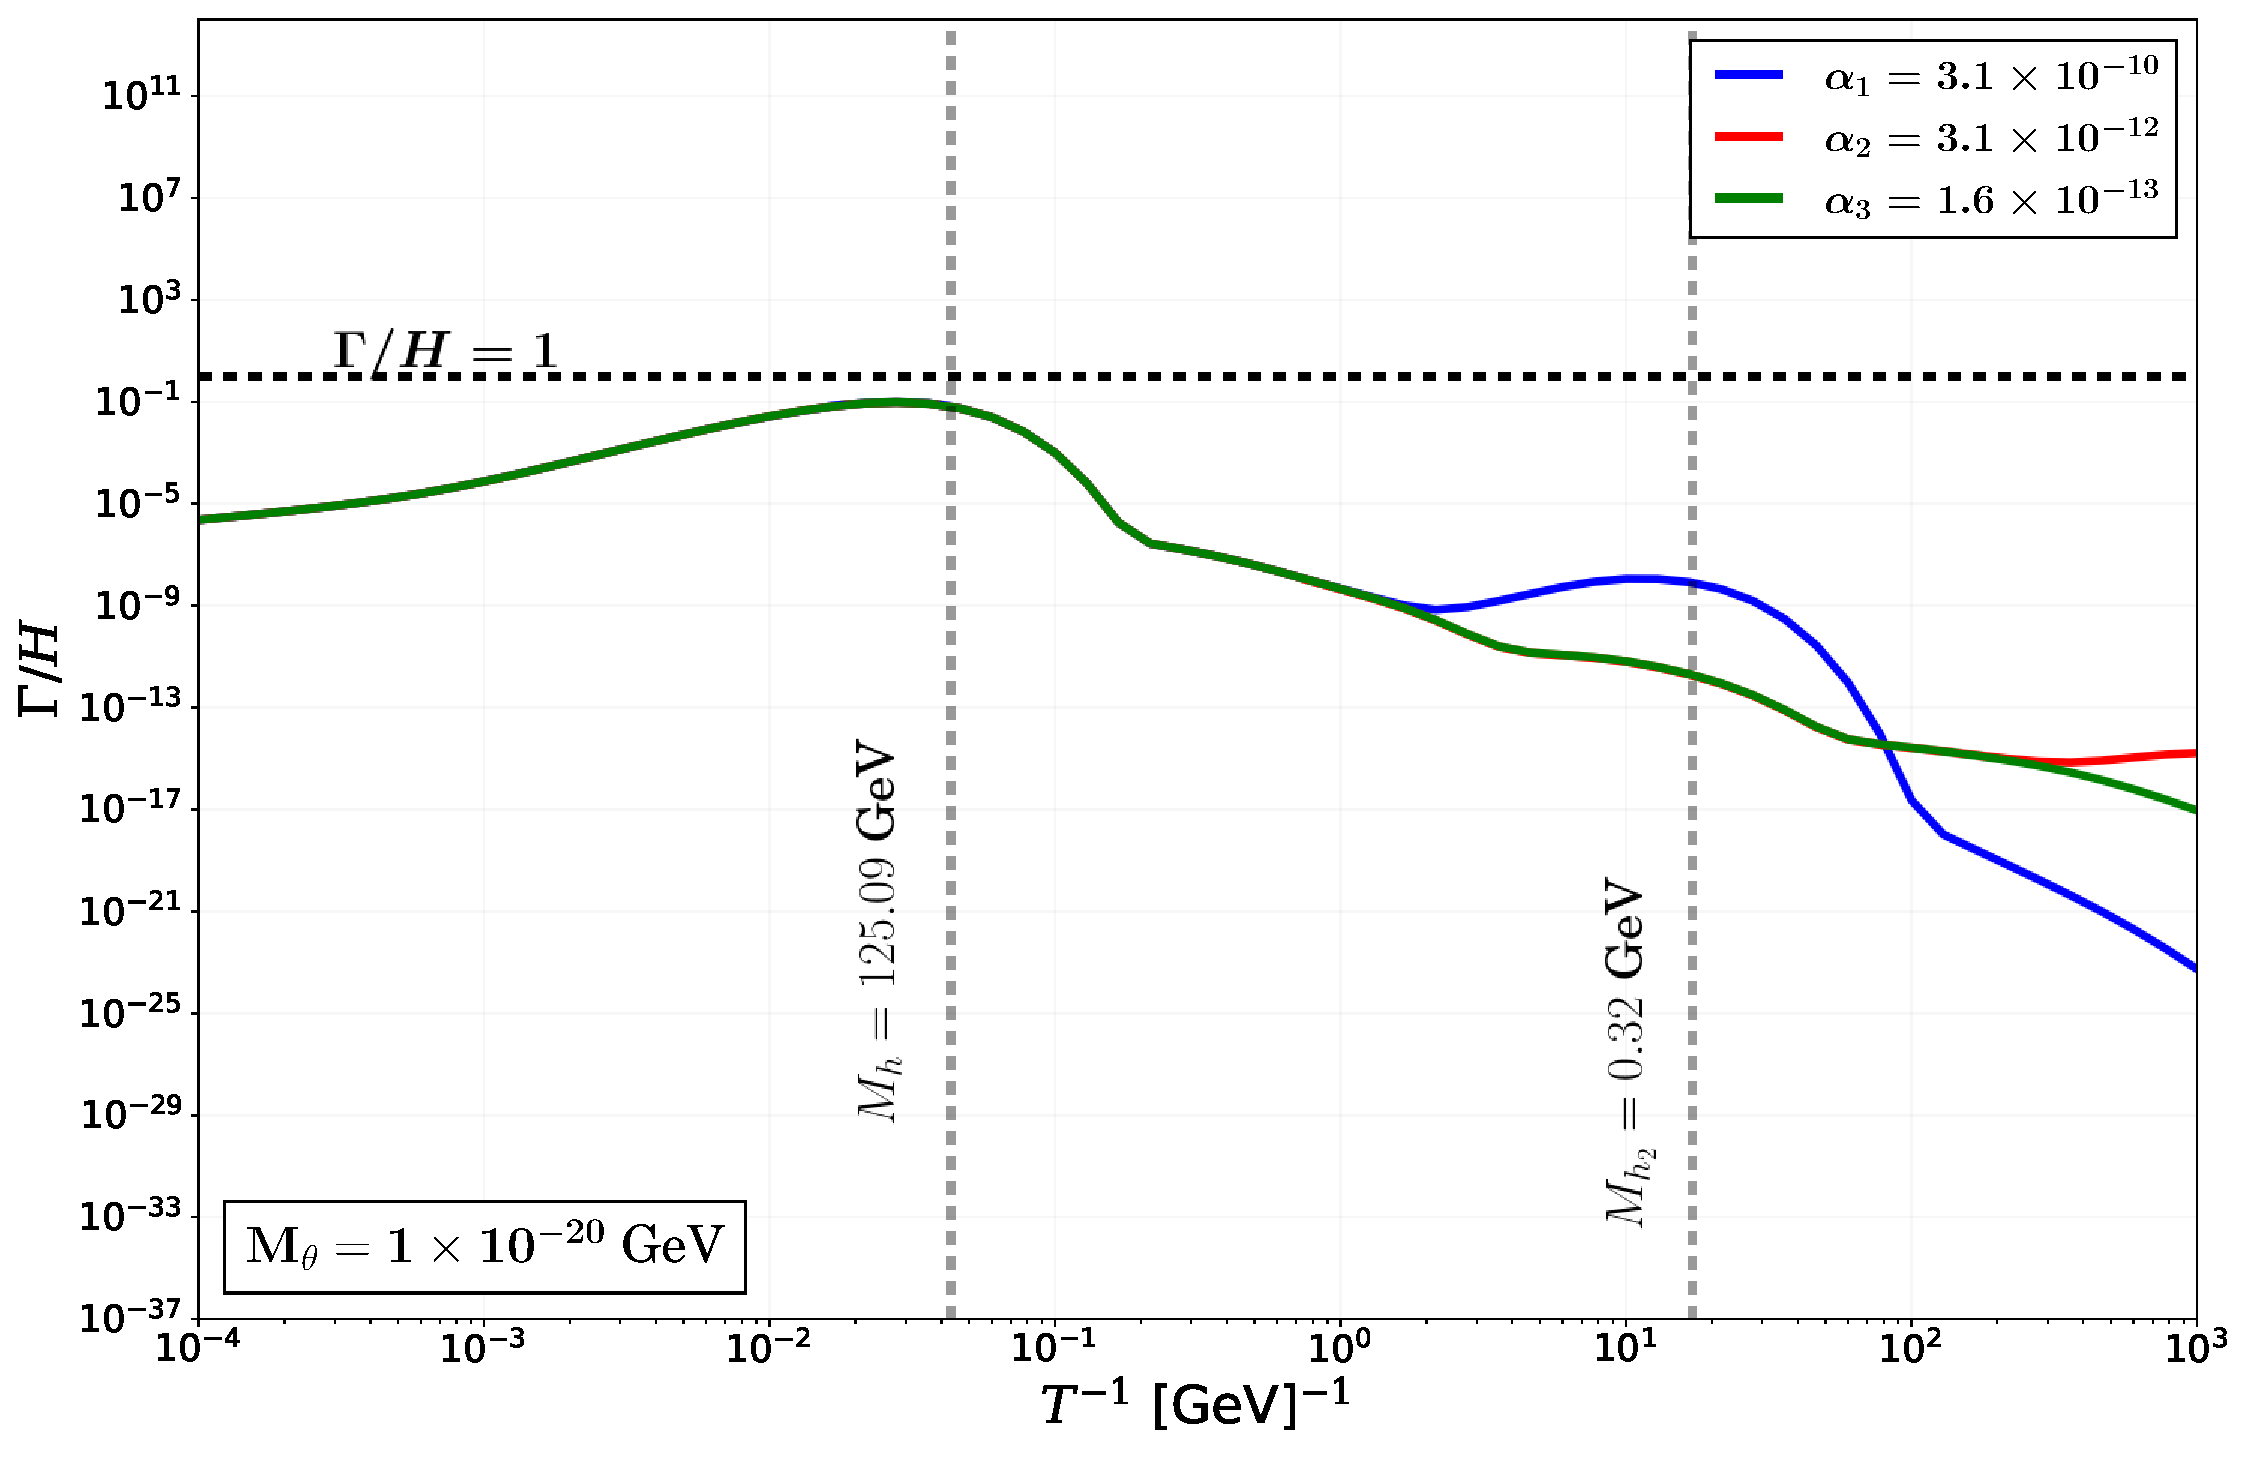
\includegraphics[width=0.7\linewidth]{graphs/ratedm_lesser}
	\caption{Rate of interaction divided by Hubble assuming $m_h \gg m_{h_2}$, for $\nu_\sigma=1$ \si{G\eV} ($M_{h_2} = 3.2\times10^{-1}$ \si{G\eV}),  $\nu_\sigma=0.01$ \si{G\eV} ($M_{h_2} = 3.2\times10^{-3}$ \si{G\eV}) and  $\nu_\sigma= 5\times10^{-4}$ \si{G\eV} ($M_{h_2} = 1.6\times10^{-4}$ \si{G\eV}), for blue, green and red curves, respectively.  Additionally, we have used $\lambda_H\sim0.26$, $\lambda_{H\phi}=2\times10^{-8}$ and $\lambda_\phi=0.1$\,.}
	\label{fig:ratelesser}
\end{figure}

\begin{figure}[H]
	\centering
	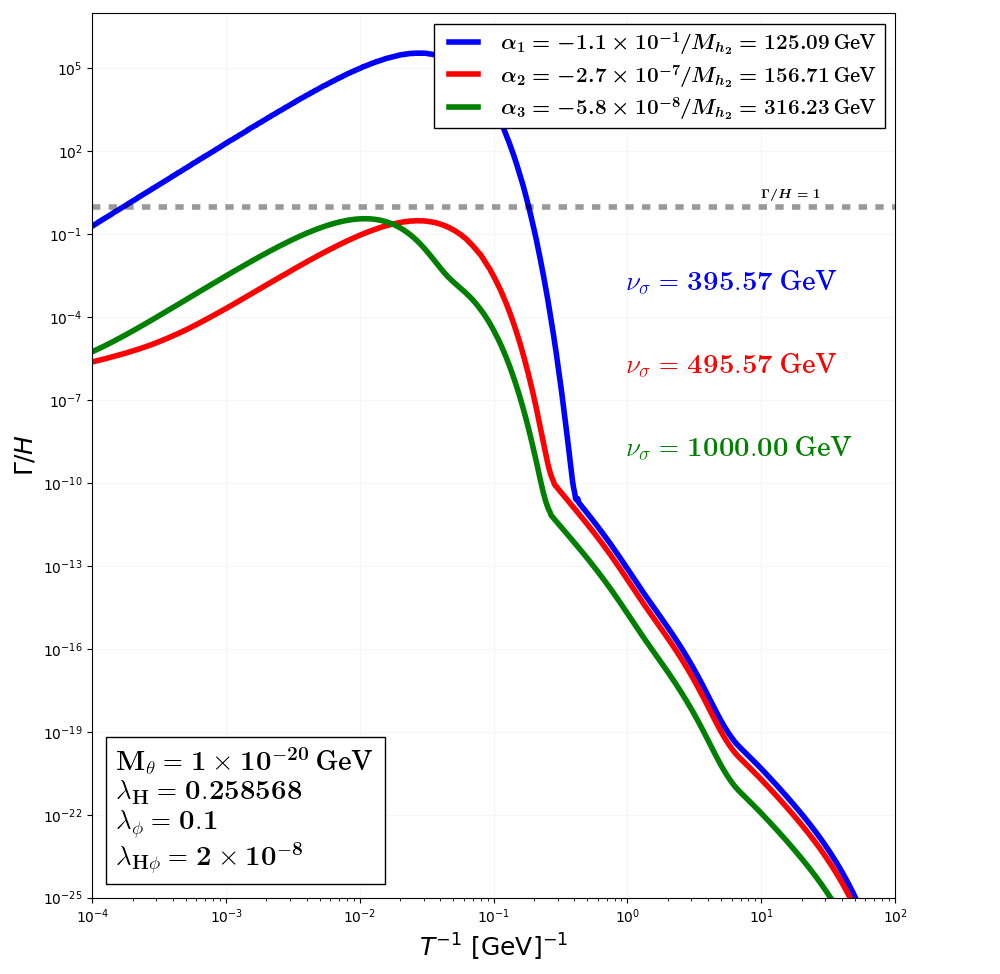
\includegraphics[width=0.75\linewidth]{graphs/ratedm_equal}
	\caption{Rate of interaction divided by Hubble assuming $m_h = m_{h_2}$, for $\nu_\sigma=395.57$ \si{G\eV} ($M_{h_2}=125.09$ \si{G\eV}),  $\nu_\sigma=495.57$ \si{G\eV} ($M_{h_2}=156.71$ \si{G\eV}) and  $\nu_\sigma=10^3$ \si{G\eV}  ($M_{h_2}=316.23$ \si{G\eV}), for blue, green and red curves, respectively.  Additionally, we have used $\lambda_H\sim0.26$, $\lambda_{H\phi}=2\times10^{-8}$ and $\lambda_\phi=0.1$\,.}
	\label{fig:rateequal}
\end{figure}

\begin{figure}[H]
	\centering
	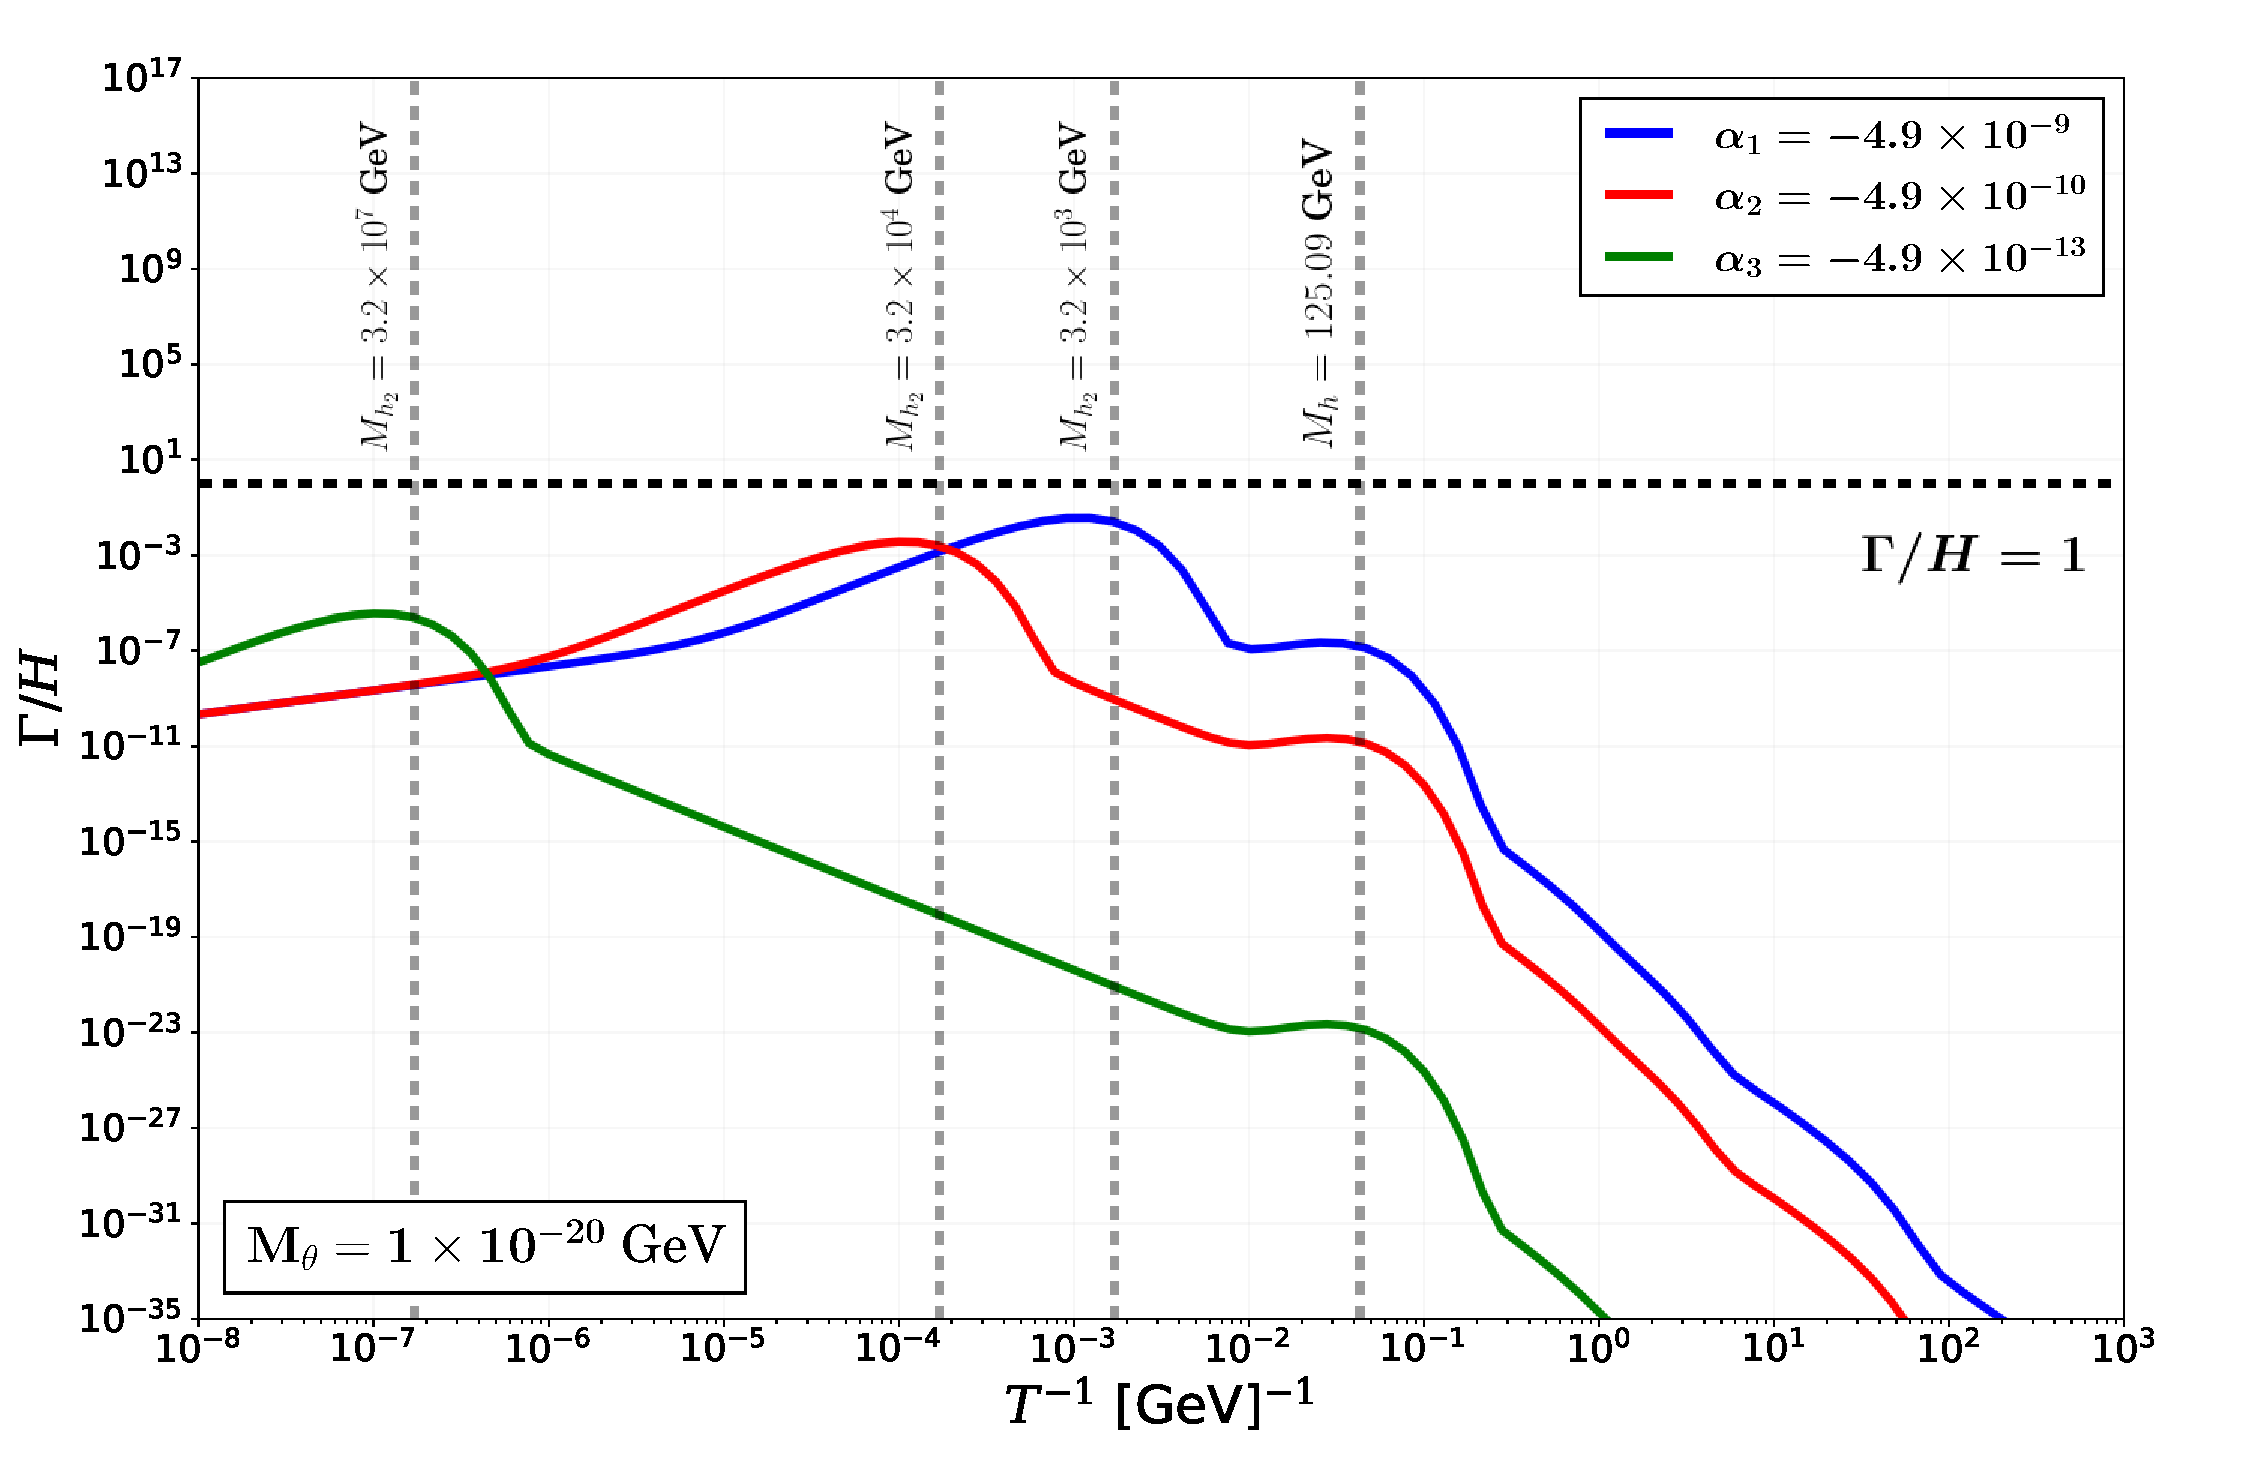
\includegraphics[width=0.8\linewidth]{graphs/ratedm_greater}
	\caption{Rate of interaction divided by Hubble assuming $m_h \ll m_{h_2}$, for $\nu_\sigma=10^4$ \si{G\eV} ($M_{h_2} = 3.2\times10^{3}$ \si{G\eV}),  $\nu_\sigma=10^5$ \si{G\eV} ($M_{h_2} = 3.2\times10^{4}$ \si{G\eV}) and  $\nu_\sigma= 10^8$ \si{G\eV} ($M_{h_2} = 3.2\times10^{7}$ \si{G\eV}), for blue, green and red curves, respectively.  Additionally, we have used $\lambda_H\sim0.26$, $\lambda_{H\phi}=2\times10^{-8}$ and $\lambda_\phi=0.1$\,.}
	\label{fig:rategreater}
\end{figure}

We can prove that as long as, the mixing angle, $\alpha\lesssim10^{-7}$, our pNGB doesn't couple with the thermal bath, and so doesn't become relativistic (cold). Notice that this constraint in the mixing angle, allows our VEV $v_\sigma$ to become a free parameter, as long as the quartic coupling terms remain the same. As mentioned in \autoref{chapter:Ultralight Bosons}, the mixing angle being small only allows decays of the $h_2$ into $\theta\theta$, and seeing as $v_\sigma$ becomes a free parameter, for large values of $v_\sigma$, this decay also disappears.

Note that there is a resonance whenever the temperature is approximately equal to the mass of the mediator, SM-Higgs or $h_2$, for $T\thicksim m_{h_{1,2}}/5.4$\cite{kolb}.

\section{Misalignment}
 
In this section, we are going to consider that the soft-symmetry breaking of the U$(1)_G$ symmetry, which produced the pNGB, occurred before the end of inflation. Inflation is a theory that explains the exponential rate of expansion of the early universe.

The temperature at which inflation occurred is bounded by the 

Using the \autoref{newvsoft}, and introducing the misalignment angle as $\Theta = \dfrac{2\theta}{v_\sigma}$
\begin{equation}
    V_{\textrm{soft}}(\Theta)\simeq \frac{m_\theta^2}{2}\left(\frac{v_\sigma}{2}\right)^2\Theta^2\,.
\end{equation}

Using the energy-momentum tensor, $T^{\mu}_\nu$, of $\theta$ 
\begin{equation}
    T^\mu_\nu=g^{\mu\alpha}(\partial_\alpha\theta)(\partial_\nu\theta)-\frac{\delta^\mu_\nu}{2}[g^{\alpha\beta}(\partial_\alpha\theta)(\partial_\beta\theta)+2V(\theta)]\,,
\end{equation}
where $g^{\mu\nu}=diag(-1,1,1,1)$ and the energy density reads as \cite{Marsh_2016}\cite{kolb}
\begin{align}
\label{densityenergy}
\begin{array}{ccc}
    &\rho_\theta=-T^0_0=-g^{0\alpha}(\partial_\alpha\theta)(\partial_0\theta)+\dfrac{1}{2}[g^{\alpha\beta}(\partial_\alpha\theta)(\partial_\beta\theta)+2V(\theta)]=\dfrac{1}{2}\left(\dfrac{\partial\theta}{\partial t}\right)^2-\dfrac{1}{2}\dfrac{\vec{\nabla}^2\theta}{a^2}+V(\theta)=\\ [5pt]
    &=\dfrac{1}{2}\left(\dfrac{\partial\theta}{\partial t}\right)^2+V(\theta)=\left(\dfrac{v_\sigma}{2}\right)^2\left[\dfrac{\dot{\Theta}^2}{2}+\dfrac{m_\theta^2}{2}\Theta^2\right]\,,
\end{array}
\end{align}
where $\theta$ only varies with time and is the same in the universe.

Knowing that the energy density of $\theta$ can be given by
\begin{equation}
\label{rhoa}
    \rho_\theta(a)=\rho_\theta(a_i)\left(\dfrac{a_i}{a}\right)^3\,,
\end{equation}
where $a$ is the scale factor, and the $a_i$ relates do any value of the scale factor.

In the radiation era of the universe, we have that, $a\propto \sqrt{t}$, where $t$ is the age of the universe.

The equation of motion for $\theta$ can be obtained varying the action, $S=\int \mathcal{L} a^3 d^4x$ , where $a$
is the scale factor, and computing the D’Alembertian for the Friedmann–Robertson–Walker (FRW) metric we obtain\cite{Marsh_2016}
\begin{equation}
\label{motion}
    \ddot{\Theta}^2+3H\dot{\Theta}+m_\theta^2\Theta=0\,.
\end{equation}

\begin{figure}[H]
	\centering
	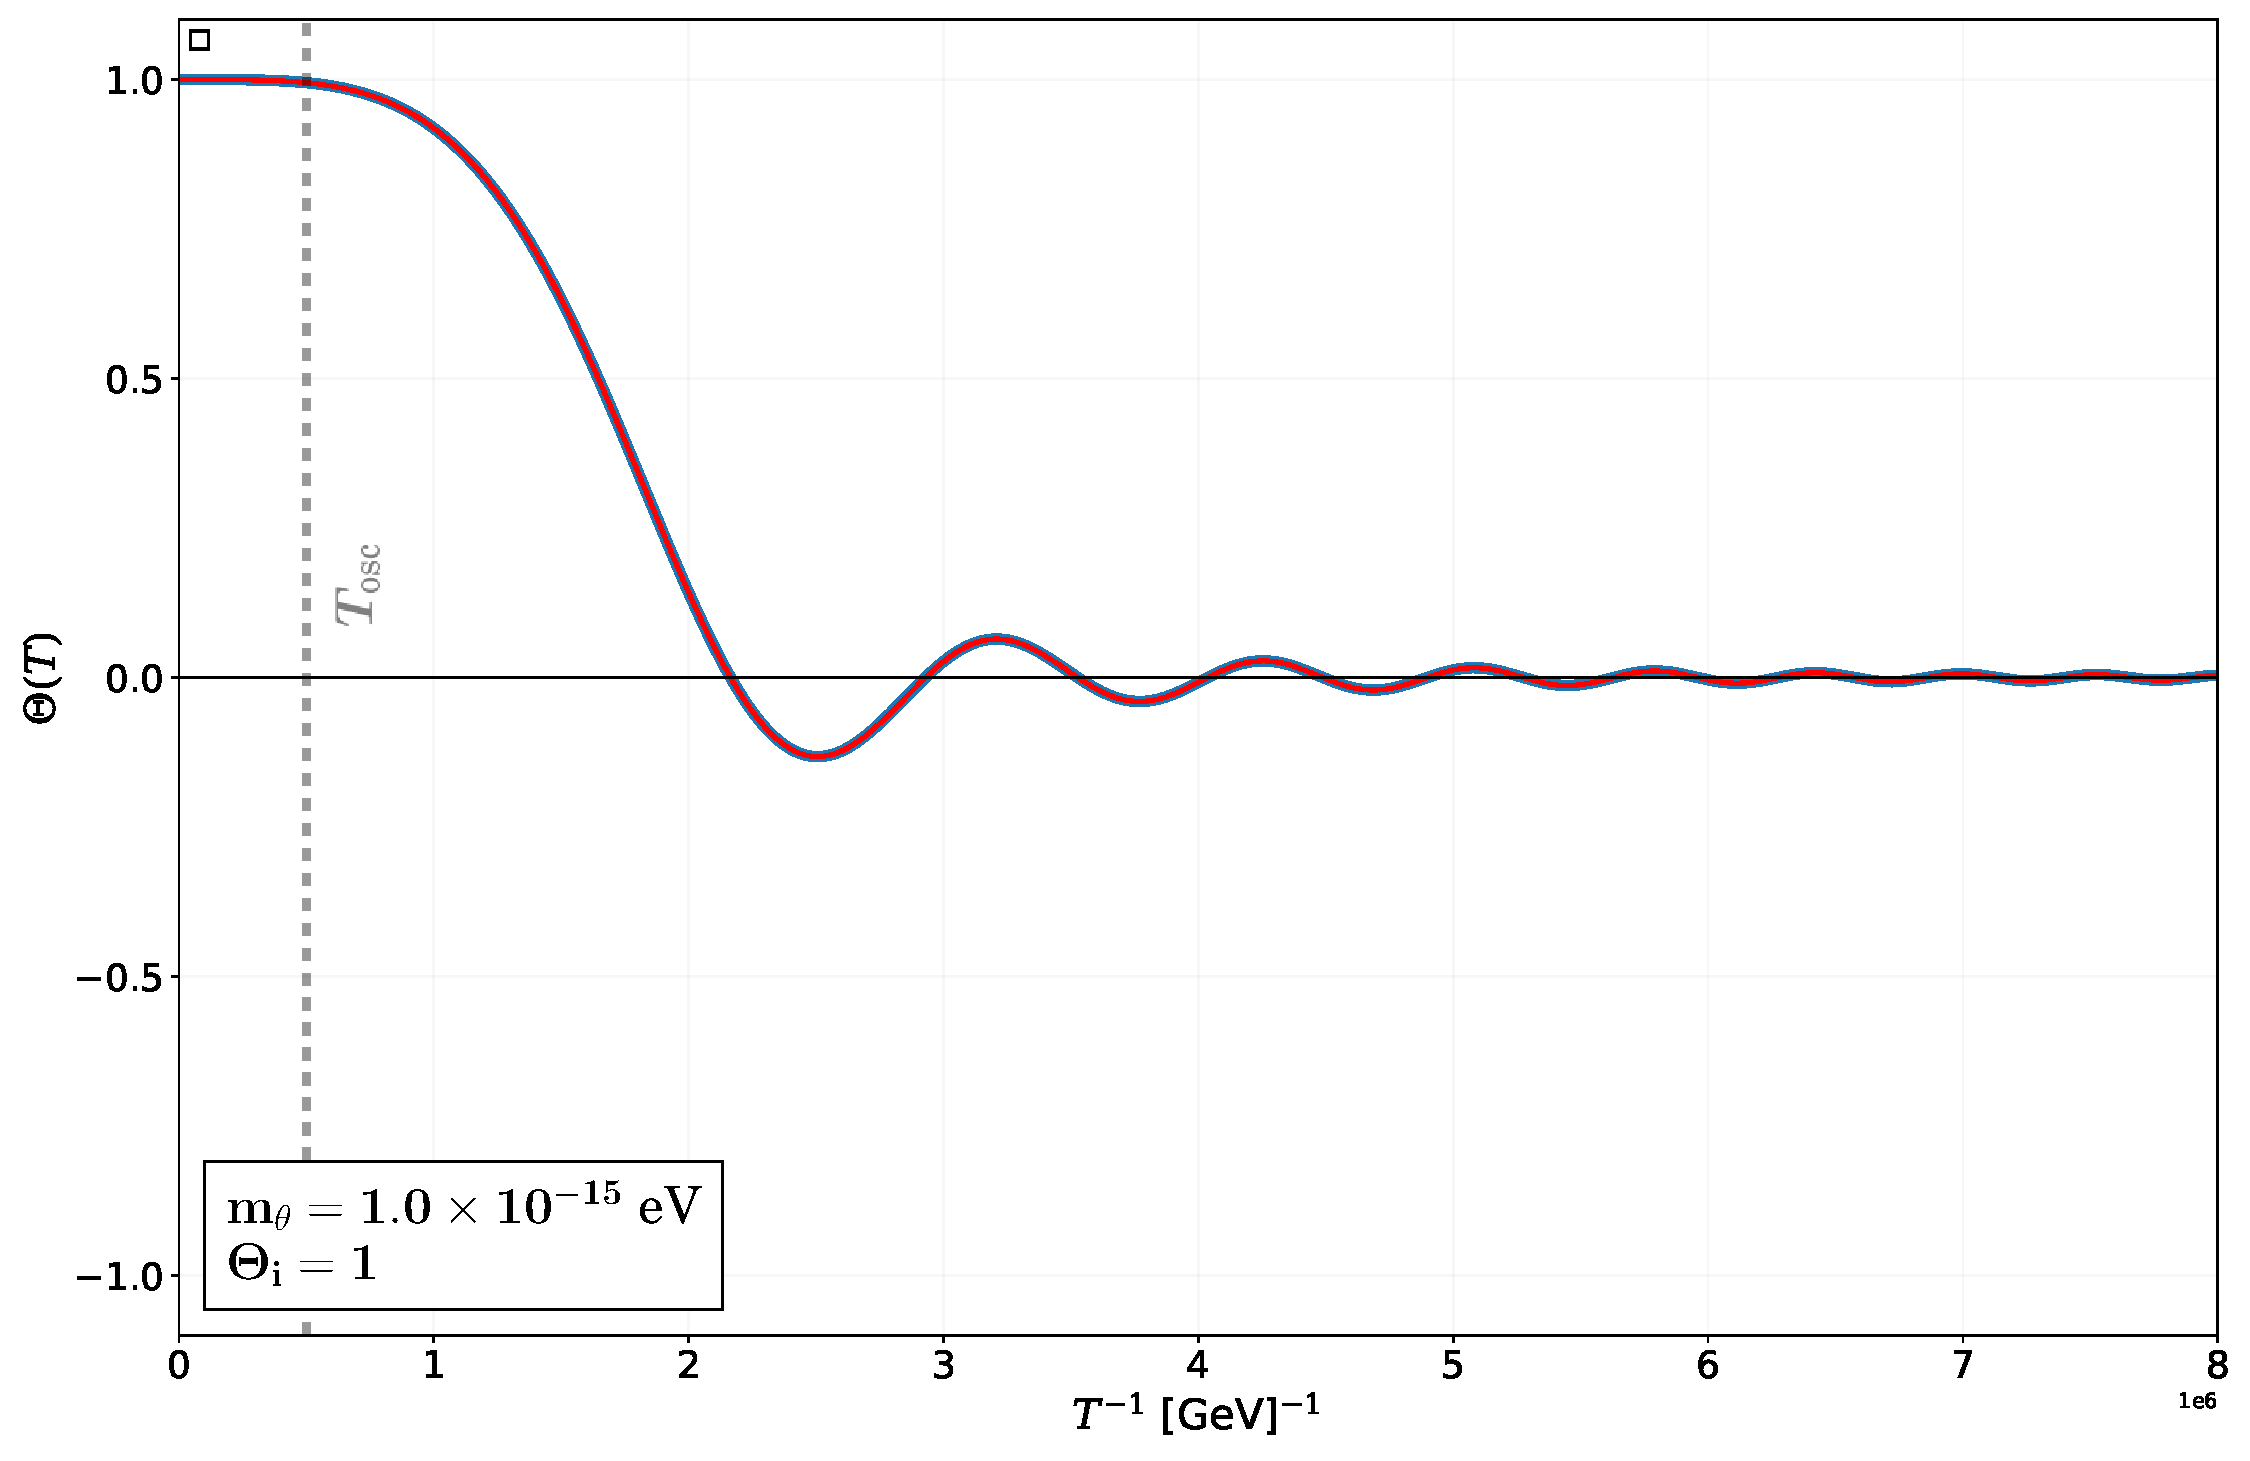
\includegraphics[width=0.9\linewidth]{graphs/motion.pdf}
	\caption{Solution of the equation of motion in \autoref{motion}\,.}
	\label{fig:motion}
\end{figure}

The \autoref{fig:motion}, allows us to see that the misalignment angle, $\Theta$, is constant for $T^{-1}\in[0,T^{-1}_{\textrm{osc}}]$, and so we can say from \autoref{densityenergy} that
\begin{equation}
    \rho_\theta(a_\textrm{osc})=\left(\dfrac{v_\sigma}{2}\right)^2\dfrac{m_\theta^2}{2}\Theta_\textrm{osc}^2\,.
\end{equation}

Using the \autoref{rhoa}, for an $a_i=a_\textrm{osc}$, we have
\begin{equation}
\label{rhoaa}
    \rho_\theta(a)=\left(\dfrac{v_\sigma}{2}\right)^2\dfrac{m_\theta^2}{2}\Theta_\textrm{osc}^2\left(\dfrac{a_\textrm{osc}}{a}\right)^3\,.
\end{equation}

Let us take a look at the entropy in the primordial universe, it can be written in terms of the pressure, $P$, and density of energy, $\rho$, as
\begin{equation}
    S=sa^3=\dfrac{\rho+P}{T}a^3\,,
\end{equation}
where $s$ is entropy density, recalling Equations (\ref{3.32}) and (\ref{eqn:3.16}) we have that the entropy can be written as
\begin{equation}
    S=\dfrac{2\pi^2}{45}g_{*s}(T)T^3a^3\,,
\end{equation}
where, $g_{*s}(T)$ is
\begin{equation}
	g_{*s}(T)=\sum\limits_{b}g_b\left(\frac{T_b}{T}\right)^3+\dfrac{7}{8}\sum\limits_{f}g_f\left(\frac{T_f}{T}\right)^3\,.
\end{equation}

Taking the following ratio,
\begin{equation}
\label{ratioS}
    \dfrac{S_\textrm{osc}}{S}=\dfrac{g_{*s}(T_\textrm{osc})}{g_{*s}(T)}\left(\dfrac{T_\textrm{osc}a_\textrm{osc}}{Ta}\right)^3\,,
\end{equation}
knowing that in the primordial universe the entropy is constant, so $S_\textrm{osc}=S$, the \autoref{ratioS} gets turned into
\begin{equation}
\label{aosc/a}
       \left(\dfrac{a_\textrm{osc}}{a}\right)^3=\dfrac{g_{*s}(T)}{g_{*s}(T_\textrm{osc})}\left(\dfrac{T}{T_\textrm{osc}}\right)^3\,.
\end{equation}

Using the \autoref{aosc/a}, the current energy density of $\theta$, in \autoref{rhoaa}, becomes
\begin{equation}
    \label{rhoaaa}
    \rho_\theta(a_0)=\left(\dfrac{v_\sigma}{2}\right)^2\dfrac{m_\theta^2}{2}\Theta_\textrm{osc}^2\dfrac{g_{*s}(T_0)}{g_{*s}(T_\textrm{osc})}\left(\dfrac{T_0}{T_\textrm{osc}}\right)^3\,.
\end{equation}
 
The current relic density of any matter is given by
\begin{equation}
    \Omega^0=\dfrac{\rho(a_0)}{\rho_\textrm{crit}}\,,
\end{equation}
and so using \autoref{rhoaaa}, the current relic density of $\theta$ reads as
\begin{equation}
    \Omega^0_\theta=\dfrac{\rho_\theta(a_0)}{\rho_\textrm{crit}}=\frac{1}{\rho_\textrm{crit}}\left(\dfrac{v_\sigma}{2}\right)^2\dfrac{m_\theta^2}{2}\Theta_\textrm{osc}^2\dfrac{g_{*s}(T_0)}{g_{*s}(T_\textrm{osc})}\left(\dfrac{T_0}{T_\textrm{osc}}\right)^3\,.
\end{equation}

This can be further simplified as we know most of this terms,  $\rho_\textrm{crit}=1.88\times 10^{-29}h^2 \si{\g\cm^{-3}}=8.1\times10^{-47}h^2$ \si{G\eV^4}, using the \autoref{masses} for $\mu_s^2=-m_\theta^2/2$, $g_{*s}(T_0)=3.91$, $g_*(T_0)=3.36$ and $T_0=2.3\times10^{-4}$ \si{\eV}, and finally we have that the current relic density of $\theta$ is
\begin{equation}
    \Omega^0_\theta h^2=0.11\left(\dfrac{m_\theta}{10^{-14}\si{\eV}}\right)^{1/2}\left(\dfrac{v_\sigma}{\sqrt{50}\times10^{17}\si{G\eV}}\right)^{2}\left(\dfrac{\Theta_\textrm{osc}}{10^{-3}}\right)^{2}\left(\dfrac{3.91}{g_{*s}(T_\textrm{osc})}\right)\left(\dfrac{g_*(T_\textrm{osc})}{3.36}\right)^{3/4}\,.
\end{equation}
 
\begin{figure}[H]
	\centering
	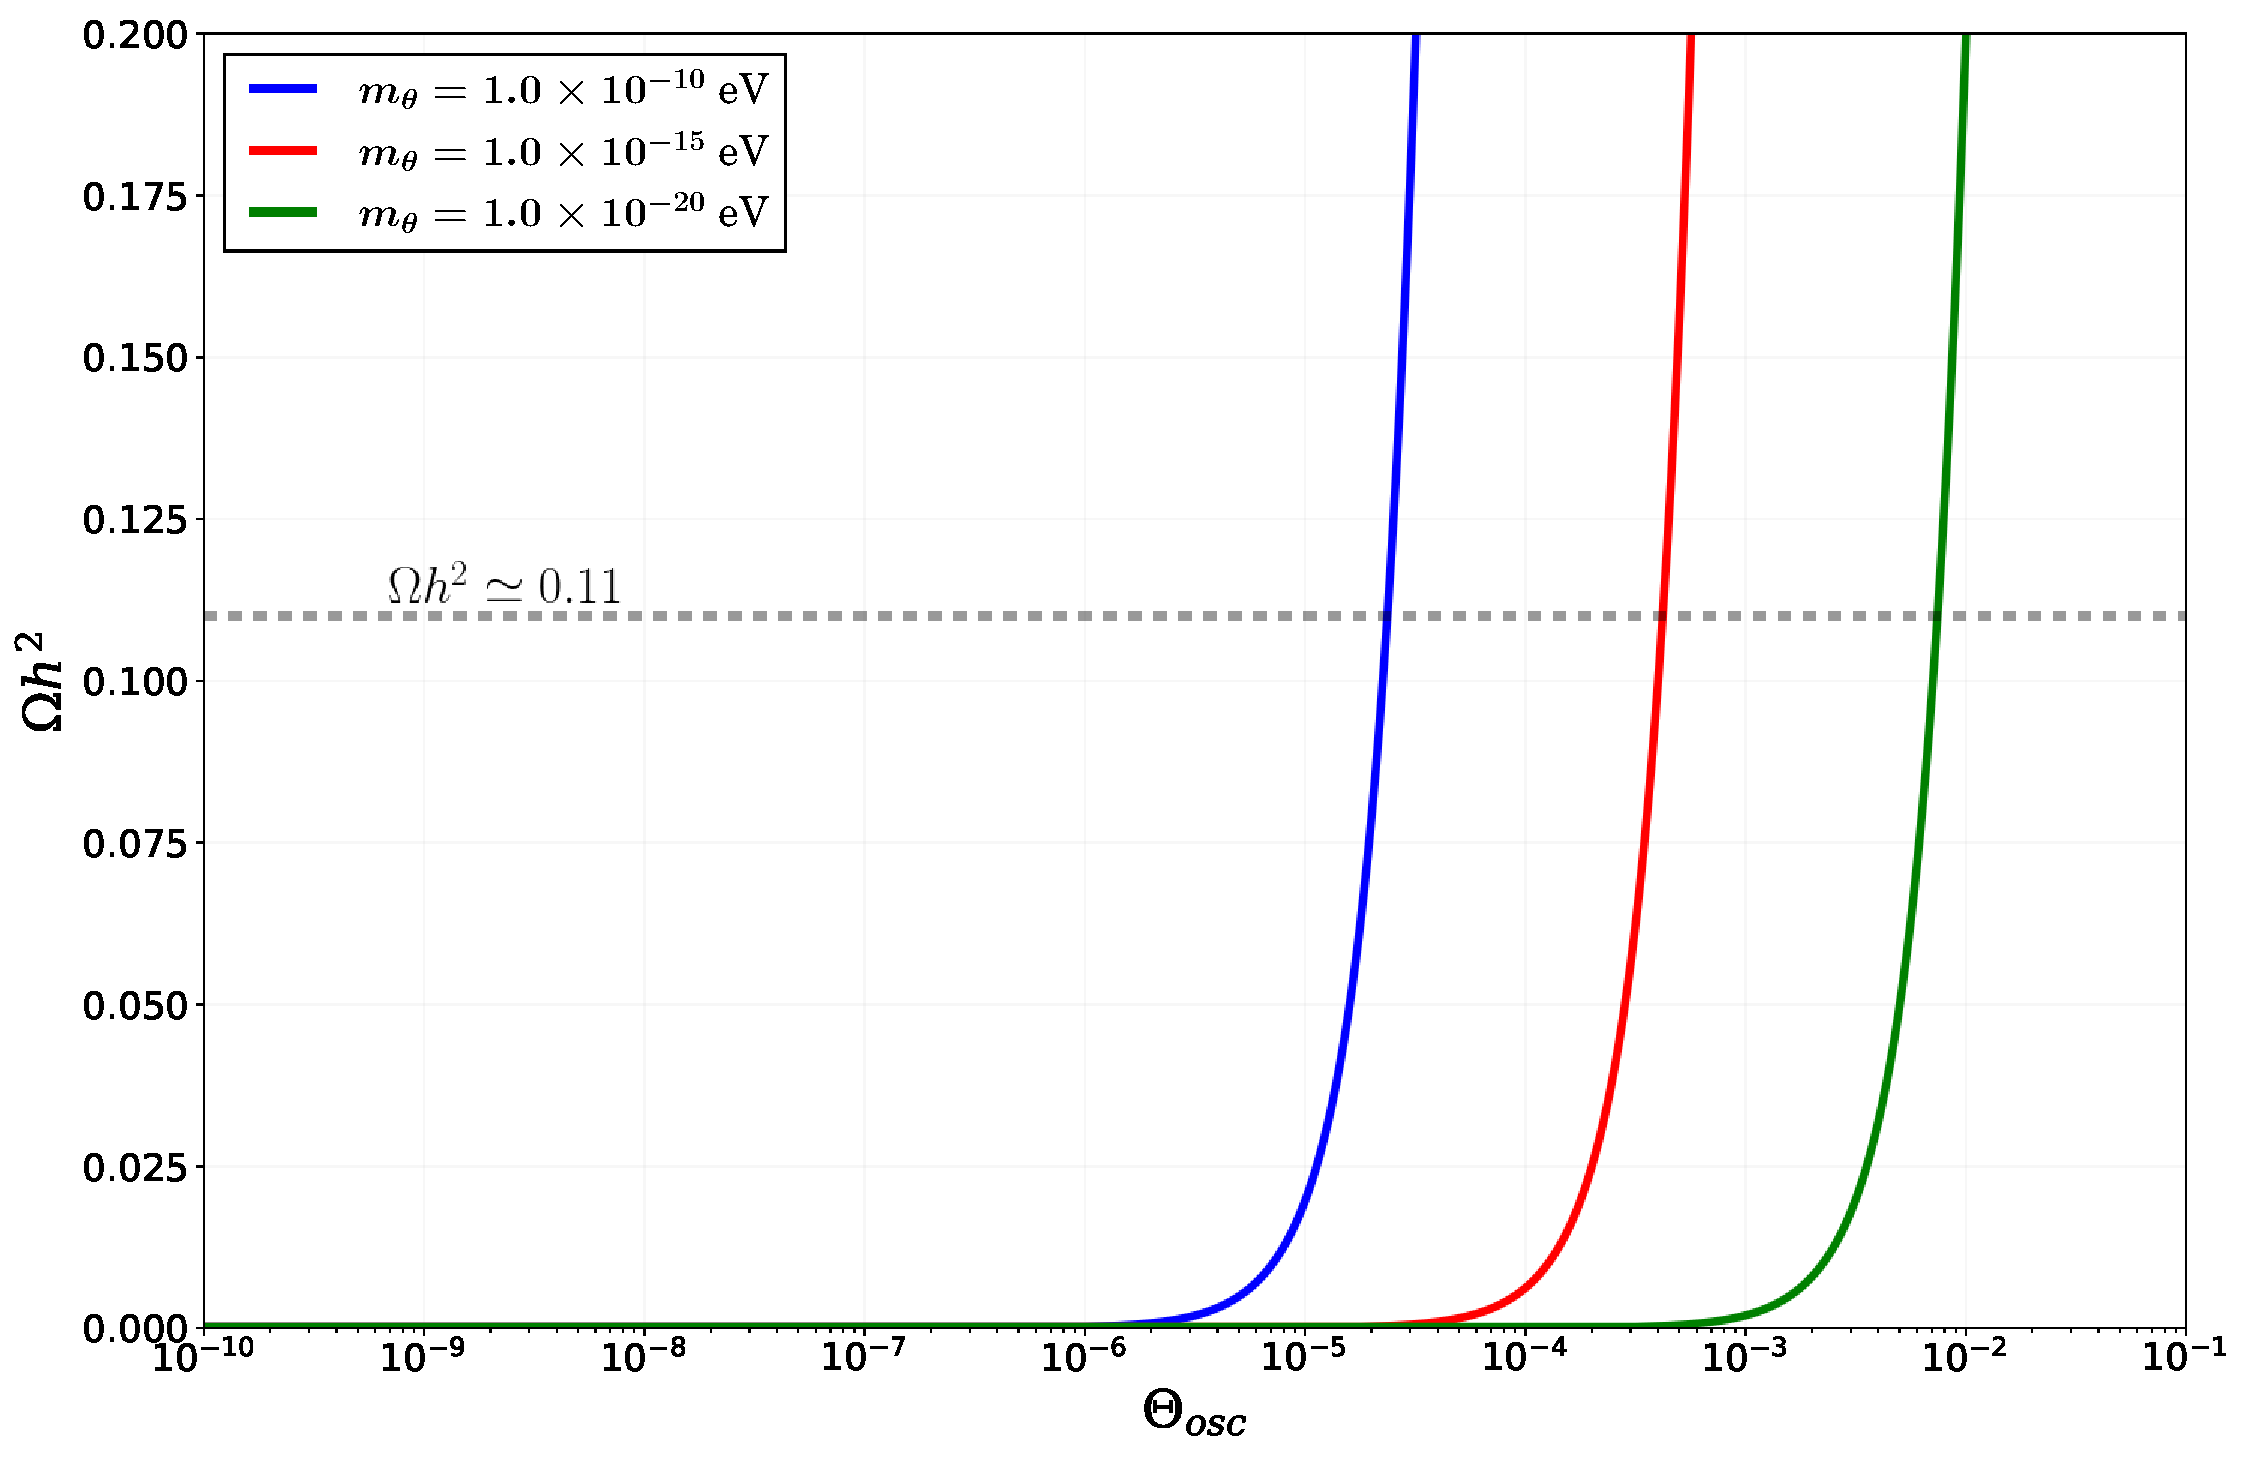
\includegraphics[width=0.9\linewidth]{graphs/relic_density.pdf}
	\caption{Relic density variating $\Theta_i$, with $v_\sigma=3\times 10^{18}$, for various values of $m_\theta$\,.}
	\label{fig:relicdesity}
\end{figure}

The \autoref{fig:relicdesity} allows us to determine the required initial misalignment angle, $\Theta_\textrm{osc}$, for certain mass and $v_\sigma$.
\chapter{Conclusion}
\label{chapter:conclusion}

In this work we took a look at an extension of the SM that allows a pGB to emerge in the physical basis, and then a brief review of the thermodynamics of the primordial universe. We were able to conclude that for a mixing angle, $\alpha\lesssim 10^{-7}$ our dark matter candidate doesn't couple with the thermal bath and therefore doesn't become relativistic. We also confirmed that any scenario where $h_2$ is heavier, equal or lighter, than the SM-Higgs, is valid.
We were also able to use the misalignment mechanism in order to find the relic density of this candidate, and say that for a value of $v_\sigma$ in the order of $\mathcal{O}(10^{18})$ its a viable option for a DM candidate.
The culmination of this work allows us to see that the pNGB is a viable candidate for DM .

%\chapter{Thermodynamics of the expanding universe}
\label{chapter:thermodynamicsofearlyuniverse}

In this chapter, our objective is to understand the evolution of the early universe, so we will make a brief review of the thermodynamics in the equilibrium of the early universe, following \cite{kolb}.

We are able to predict how the universe behaved due to the Cosmic Microwave Background (CMB) being approximately equal to the spectra of a black body, so we assume that in the primordial universe the particles from the SM are in equilibrium.

\section{Thermodynamics in equilibrium}
The number density, $n$, energy density, $\rho$, and the pressure, $P$ of a gas of particles with a degree of freedom, $g$, distinguish the thermodynamic properties of the gas and are defined as a function of the distribution function $f(\vec{p},t)$:
\begin{equation}
	\label{eqn:3.1}
	n(t)\equiv\frac{g}{(2\pi)^3}\int f(\vec{p},t) d\vec{p}\,,
\end{equation}
\begin{equation}
	\label{eqn:3.2}
	\rho(t)\equiv\frac{g}{(2\pi)^3}\int E(\vec{p})f(\vec{p},t) d\vec{p}\,,
\end{equation} 
\begin{equation}
	\label{eqn:3.3}
	P(t)\equiv\frac{g}{(2\pi)^3}\int \frac{p^2}{3E}f(\vec{p},t) d\vec{p}\,,
\end{equation}  
where $\vec{p}=(p_x,p_y,p_z)$, $d\vec{p}\equiv dp_xdp_ydp_z$ and E=$\sqrt{p^2+m^2}$. The phase pace equilibrium distribution function for a particle $i$ will be given by one of the three following distributions
\begin{equation}
	f_i^{eq} = \left\{ 
	\begin{array}{lll}
		\frac{1}{e^{(E_i-\mu_i)/T}+1}\,, \quad\textrm{Fermi-Dirac}\,,\\
		\frac{1}{e^{(E_i-\mu_i)/T}-1}\,, \quad\textrm{Bose-Einstein}\,,\\
		e^{-(E_i-\mu_i)/T}\,, \quad \textrm{Maxwell-Boltzmann}\,,	
	\end{array}
	\right.
\end{equation}
where $E_i$ and $\mu_i$ is the energy and chemical potential of the particle $i$, respectively. The Fermi-Dirac (Bose-Einstein) statistic refers to particles with half-integer (integer) spin.

Using spherical symmetry we can simplify, $d\vec{p}=4\pi p^2dp,$ we can now rewrite the Equations (\ref{eqn:3.1}), (\ref{eqn:3.2}) and (\ref{eqn:3.3}) in function of the energy, $E$, given as
\begin{equation}
	\label{eqn:3.5}
	n_R=\frac{g}{2\pi^2}\int_{m}^{\infty} \frac{(E^2-m^2)^{1/2}}{e^{(E-\mu)/T}\pm 1}dE\,,
\end{equation}
\begin{equation}
	\label{eqn:3.6}
	\rho_R=\frac{g}{2\pi^2}\int_{m}^{\infty} \frac{(E^2-m^2)^{1/2}}{e^{(E-\mu)/T}\pm 1}E^2dE\,,
\end{equation} 
\begin{equation}
	\label{eqn:3.7}
	P_R=\frac{g}{6\pi^2}\int_{m}^{\infty} \frac{(E^2-m^2)^{3/2}}{e^{(E-\mu)/T}\pm 1}dE\,,
\end{equation}
where "R"\ refers to radiation, the inferior limit of the integral refers to the lowest energy a particle can have, which is its mass, $m$.

Let's take a look at a generalized solution for the Fermi-Dirac and Bose-Einstein distributions, when we take into account that the mass of the particle is so low such that, $m \simeq 0$, we get
\begin{equation}
	\nonumber
	\int_{m}^{\infty} \frac{(E^2-m^2)^s}{e^{(E-\mu)/T}\pm 1}dE =  	\int_{0}^{\infty}\frac{E^s}{e^{\frac{E-\mu_i}{T}}\pm 1}dE\,,
\end{equation}
by making $k=\frac{E}{T}$ and $\mu=\frac{\mu_i}{T}$, we get \cite{fermi}\cite{bose}
\begin{equation}
	\label{eqn:3.8}
	\int_{0}^{\infty}\frac{E^s}{e^{\frac{E-\mu_i}{T}}\pm 1}dE =\int_{0}^{\infty}\frac{(Tk)^s}{e^{k-\mu}\pm 1}Tdk=T^{s+1}\int_{0}^{\infty}\frac{k^s}{e^{k-\mu}\pm 1}dk=\mp T^{s+1} \Gamma(s+1)Li_{1+s}(\mp e^\mu)\,,
\end{equation}
where the polylogarithm or Jonquière's function and the Gamma function, are respectively defined by \cite{poly}
\begin{equation}
	\label{eqn:3.9}
	Li_n(z)\equiv\sum\limits_{k=1}^\infty \frac{z^k}{k^n} \quad \textrm{and} \quad \Gamma(s+1)=\int_{0}^{\infty} e^{-x}x^s dx=s!\,.
\end{equation}

At the ultra-relativistic limit (radiation), $T\gg m,\mu_i$. We can simplify $\mu=\mu_i/T \simeq 0$ and so the polylogarithm function in \autoref{eqn:3.8} can be simplified into
\begin{equation}
	\label{eqn:3.10}
	Li_{s+1}(\mp 1)=\sum\limits_{k=1}^{\infty}\frac{(\mp1)^k}{k^{s+1}}\,,
\end{equation}
now if we take a look at the solution of the following sum
\begin{equation}
	\label{eqn:3.11}
	\sum\limits_{k=1}^{\infty}\frac{(-1)^{k+1}}{k^s}=(1-2^{-s})\zeta(s+1)\,,
\end{equation}
where $\zeta(s)$ the Riemann zeta function, defined by
\begin{equation}
	\label{eqn:3.12}
	\zeta(s)=\sum\limits_{k=1}^{\infty}\frac{1}{k^s}\,,
\end{equation}
using the solutions in Equations (\ref{eqn:3.11}) and (\ref{eqn:3.12}) the generalized solution for ultra-relativistic particles, in \autoref{eqn:3.8}, gets reduced to 
\begin{equation}
	\int_{0}^{\infty}\frac{E^s}{e^{\frac{E-\mu_i}{T}}\pm 1}dE=\left\{ \begin{array}{c}
		T^{s+1}(1-2^{-s})\zeta(s+1)s!\,, \quad \textrm{Fermi-Dirac}\,, \\
		T^{s+1}\zeta(s+1)s!\,, \quad \textrm{Bose-Einstein}\,,	
	\end{array}\right.\,.
\end{equation}
Now we can easily integrate the Equations (\ref{eqn:3.5}), (\ref{eqn:3.6}) and (\ref{eqn:3.7}), knowing that $\zeta(4)=\pi^4/90$ to
\begin{equation}
	\label{eqn:3.14}
	n_{\textrm{R}}=\frac{g}{2\pi^2}\int_{0}^{\infty} \frac{E}{e^{E/T}\pm1}dE=\frac{g}{\pi^2}T^3\zeta(3)\left\{ \begin{array}{c}
		3/4\,, \quad \textrm{Fermi-Dirac}\,, \\
		1\,, \quad \textrm{Bose-Einstein}\,,
	\end{array}\right.
\end{equation}
\begin{equation}
	\label{eqn:3.15}
	\rho_{\textrm{R}}=\frac{g}{2\pi^2}\int_{0}^{\infty} \frac{E^3}{e^{E/T}\pm1}dE=g\frac{\pi^2}{30}T^4\left\{ \begin{array}{c}
		7/8\,,\quad \textrm{Fermi-Dirac}\,, \\
		1\,, \quad \textrm{Bose-Einstein}\,,
	\end{array}\right.
\end{equation} 
\begin{equation}
	\label{eqn:3.16}
	P_{\textrm{R}}=\frac{g}{6\pi^2}\int_{0}^{\infty} \frac{E^3}{e^{E/T}\pm1}dE=\frac{1}{3}\rho_{\textrm{R}}\,,
\end{equation}  
where the + and - refers respectively to the Fermi-Dirac and Bose-Einstein distributions.

Now let's take a look at the non-relativistic limit (matter), $T \ll m,\mu$, which follows the Maxwell-Boltzmann distribution, we can rewrite the Equations (\ref{eqn:3.1}), (\ref{eqn:3.2}) and (\ref{eqn:3.3}) in function of the momentum, $p$, given as

\begin{equation}
	\label{eqn:3.17}
	n_{\textrm{M}}\equiv\frac{g}{(2\pi)^3}\int e^{-\frac{(E-\mu)}{T}} d\vec{p}\,,
\end{equation}
\begin{equation}
	\label{eqn:3.18}
	\rho_{\textrm{M}}\equiv\frac{g}{(2\pi)^3}\int E(\vec{p})e^{-\frac{(E-\mu)}{T}} d\vec{p}\,,
\end{equation} 
\begin{equation}
	\label{eqn:3.19}
	P_{\textrm{M}}\equiv\frac{g}{(2\pi)^3}\int \frac{p^2}{3E}e^{-\frac{(E-\mu)}{T}} d\vec{p}\,,
\end{equation}  
where the subscript "M"\ means Matter (non-relativistic limit).

Let's take a look at a generalized solution to a certain integral, where we use spherical coordinates, $d\vec{p}=4\pi p^2 dp$
\begin{equation}
\label{eqn:3.20}
	\int p^k E^s e^{-\frac{(E-\mu)}{T}} d\vec{p}=4\pi e^{\mu/T}T^s\int_{0}^{\infty} p^{k+2} \frac{(p^2+m^2)^{s/2}}{T^s} e^{-\frac{\sqrt{p^2+m^2}}{T}} dp\,,
\end{equation}
substituting $x=\frac{p}{T}$ and $\gamma=\frac{\mu}{T}$, in \autoref{eqn:3.20}
\begin{equation}
	\label{eqn:3.21}
	4\pi e^{\mu/T}T^{s+k+3}\int_{0}^{\infty} x^{k+2}(x^2+\gamma^2)^{s/2}e^{-\sqrt{x^2+\gamma^2}} dx\,,
\end{equation}
by taking into account $T \ll m,\mu$, we can do the following approximation to simplify the integration
\begin{equation}
\label{eqn:3.22}
	(x^2+\gamma^2)^{s/2}=\gamma^s\left[1+\left(\frac{x}{\gamma}\right)\right]^{s/2} \approx \gamma^s+\frac{s}{2}\gamma^{s-2}x^2\,,
\end{equation}
then using Eq.(\ref{eqn:3.22}), the \autoref{eqn:3.21} becomes
\begin{equation}
	\label{eqn:3.23}
	4\pi e^{\mu/T}T^{s+k+3}\gamma^se^{-\gamma}\left[ \int_{0}^{\infty} x^{k+2}e^{-\frac{x^2}{2\gamma}}dx+\frac{s}{2}\gamma^{-2}\int_{0}^{\infty} x^{k+4}e^{-\frac{x^2}{2\gamma}}dx\right]\,,
\end{equation}
from Eq.(\ref{eqn:3.23}), $u=\frac{x^2}{2\gamma}$,
\begin{equation}
	4\pi e^{\mu/T}T^{s+k+3}\gamma^{s+1}e^{-\gamma}\left[(2\gamma)^{\frac{k+1}{2}}\int_{0}^{\infty} u^{(k+1)/2}e^{-u}du+\frac{s}{2}\gamma^{-2}(2\gamma)^{\frac{k+3}{2}}\int_{0}^{\infty} u^{(k+3)/2}e^{-u}du\right]\,,
\end{equation}
using the Gamma function, as shown in \autoref{eqn:3.9}, the \autoref{eqn:3.20}) becomes

\begin{equation}
	\label{eqn:3.24}
	4\pi T^{s+k+3}e^{-\frac{(m-\mu)}{T}} 2^{(k+1)/2} \left( \frac{m}{T}\right)^{\frac{k+3}{2}+s}
	\left[\left((k+1)/2\right)!+\frac{s}{2}\left(\frac{m}{T}\right)^{-1}\left((k+3)/2\right)!\right]\,.
\end{equation}

We can now determine the Equations (\ref{eqn:3.17}), (\ref{eqn:3.18}) and (\ref{eqn:3.19}), and so we get these solutions, knowing that $(1/2)!=\sqrt{\pi}/2$,
\begin{equation}
	\label{nM}
	n_{\textrm{M}}=\frac{g}{(2\pi)^3}\int e^{-\frac{(E-\mu)}{T}} d\vec{p}=g\left( \frac{mT}{2\pi}\right)^{\frac{3}{2}}e^{-\frac{(m-\mu)}{T}}\,,
\end{equation}
\begin{equation}
	\label{rhoM}
	\rho_{\textrm{M}}=\frac{g}{(2\pi)^3}\int E(\vec{p})e^{-\frac{(E-\mu)}{T}} d\vec{p}=n_{M}m\left[1+\frac{3}{2}\left(\frac{T}{m}\right)\right]\,,
\end{equation} 
\begin{equation}
	\label{PM}
	P_{\textrm{M}}=\frac{g}{(2\pi)^3}\int \frac{p^2}{3E}e^{-\frac{(E-\mu)}{T}} d\vec{p}=n_{M} 
	T\left[1-\frac{5}{6}\left(\frac{T}{m}\right)\right]\,.
\end{equation}


Assuming a period when $T \sim$ \SI{300}{G\eV}, and so during this time we can easily notice that $T\gg m,\mu$ and so the total energy density is equal to the sum of the energy density for each relativistic specie
\begin{equation}
	\rho_{\textrm{Total}}=\sum\limits_{i} \rho_\textrm{R}^{(i)}\,,
\end{equation}
where $i$ represents particles of the SM.

As the universe expands, its temperature decreases and so some particles become non-relativistic, behave accordingly to the Maxwell Boltzmann distribution, when $T \sim m$, and so the energy density of matter increases, so we can represent the energy density of the universe as
\begin{equation}
	\rho_{\textrm{Total}}=\sum\limits_{i}\rho_{\textrm{R}}^{(i)}+\sum\limits_{j}\rho_{\textrm{M}}^{(j)}\,,
\end{equation}
where $i$ and $j$ represent relativistic and non-relativistic particles, respectively.

Although some particles become non-relativistic as the temperature decreases, their contribution becomes negligible because their energy density, $\rho_{\textrm{M}}$, decreases exponentially as shown in Eq.(\ref{rhoM}), and so we can approximate the energy density in the primordial universe to
\begin{equation}
	\rho_{\textrm{Total}}\simeq\sum\limits_{i}\rho_{\textrm{R}}^{(i)}\,.
\end{equation}

Taking into account that species of particles can evolve with different temperatures, even in equilibrium, we can write the $\rho_{\textrm{R}}$ in terms of the temperature of photons, $T$, as follows

\begin{equation}
\label{3.32}
	\rho_{\textrm{R}}=\sum\limits_{b}\rho_{b}+\sum\limits_{f}\rho_{f}=\frac{\pi^2}{30}T^4g_*(T)\,,
\end{equation}
where, "b"\ stands for bosons, "f"\ stands for fermions, and $g_*(T)$ is
\begin{equation}
	g_*(T)=\sum\limits_{b}g_b\left(\frac{T_b}{T}\right)^4+\dfrac{7}{8}\sum\limits_{f}g_f\left(\frac{T_f}{T}\right)^4\,,
\end{equation}
putting away the photon and neutrinos we can write this as
\begin{equation}
	\nonumber
	\rho_{\textrm{R}}=\frac{\pi^2}{30}T^4\left[g_\gamma+\frac{7}{8}\sum\limits_{\nu}g_\nu\left(\frac{T_\nu}{T}\right)^4+\sum\limits_{b}g_b\left(\frac{T_b}{T}\right)^4+\frac{7}{8}\sum\limits_{f}g_f\left(\frac{T_f}{T}\right)^4\right]=
\end{equation}
\begin{equation}
	\nonumber
	=\rho_\gamma\left[1+\frac{1}{g_\gamma}\frac{7}{8}\left(\frac{T_\nu}{T}\right)^4\left(\sum\limits_{\nu}g_\nu+\sum\limits_{b}g_b\left(\frac{T_b}{T_\nu}\right)^4+\sum\limits_{f}g_f\left(\frac{T_f}{T_\nu}\right)^4\right)\right]\,,
\end{equation}
where $\rho_\gamma$ is
\begin{equation}
	\rho_\gamma=\frac{\pi^2}{30}T^4g_\gamma\,,
\end{equation}
and finally, we get
\begin{equation}
	\rho_{\textrm{R}}=\rho_\gamma\left[1+\frac{7}{8}\left(\frac{T_\nu}{T}\right)^4N_\textrm{eff}\right]\,,
\end{equation}
where $N_\textrm{eff}$ is the effective number of ultra-relativistic species ignoring the photon, and $g_\gamma=2$, as is given by
\begin{equation}
	N_\textrm{eff}=\frac{1}{g_\gamma}\left(\sum\limits_{\nu}g_\nu+\sum\limits_{b}g_b\left(\frac{T_b}{T_\nu}\right)^4+\sum\limits_{f}g_f\left(\frac{T_f}{T_\nu}\right)^4\right)\,,
\end{equation}
experiments using the CMB determine $N_\textrm{eff}=2.99 \pm 0.14$\cite{2020}.


\section{Collision Operator}
In the early universe, its contents were for the most part in thermal equilibrium, so it's a good approximation of making it in equilibrium, following \cite{kolb}.

The Boltzmann equation which describes the microscopic evolution of a particle's phase space distribution function $f(p^\mu,x^\mu)$, is given by:
\begin{equation}
	\hat{L}[f]=C[f]\,,
\end{equation}
where $\hat{L}$ is the Liouville operator and $C$ is the collision operator.


The collision operator for a process of annihilation while focusing on the particle 1 ($1 + 2 \Leftrightarrow 3 + 4$) is given by
\begin{align}
	\label{eqn:3.38}
	\begin{array}{lll}
		\dfrac{g}{(2\pi)^3}\mathlarger{\int} C[f_1]\dfrac{d^3p_1}{E_1}
		&=\pm \mathlarger{\int} (2\pi)^4 \delta^4(\mathcal{P}_1 + \mathcal{P}_2 - \mathcal{P}_3 - \mathcal{P}_4)\\[15pt]
		&\times[|\overline{M}|^2_{1 + 2 \rightarrow 3 + 4}f_1 f_2 (1\pm f_3)(1\pm f_4) \\ [15pt]
		&-|\overline{M}|^2_{3 + 4 \rightarrow 1 + 2}f_3 f_4 (1\pm f_1)(1\pm f_2) ] d\Pi_1 d\Pi_2 d\Pi_3 d\Pi_4\,,
	\end{array}
\end{align}
where $\mathcal{P}_i=(E_i,\vec{p}_i)$, $d\Pi_i=\dfrac{g_i d\vec{p}_i}{2(2\pi)^3E_i}$, the $\pm$ refers to which direction the process takes, where + refers to the production of the particle 1 ($3+4\rightarrow1+2$) and - refers to it's consumption ($1+2\rightarrow 3+4$), in the term $(1\pm f_i)$, the + appears when $i$ is a boson and - when it's a fermion, and $|\overline{M}|^2$ is the mean of initial and final spins squared.
In order to simplify we are going to assume
\begin{equation}
	|\overline{M}|^2 \equiv |\overline{M}|^2_{1+2\rightarrow 3+4} \equiv |\overline{M}|^2_{3+4\rightarrow 1+2} \,,
\end{equation}
this assumption is well explained in \cite{kolb}.

The amplitude is defined as
\begin{equation}
	|\overline{M}|^2=\frac{S_{12}S_{34}}{g_1g_2g_3g_4}|M|^2\,,
\end{equation} 
where $|M|^2$ is the amplitude squared of the processes, and the symmetrization factor $S_{i,j}=1/n_{i,j}!$ which accounts for identical particles, if the particles $i$ and $j$ are the same, $S_{i,j}=0.5$ and if they are different $S_{i,j}=1$ (note that even particles and anti-particles are different particles). 
If we assume that the particle $i$ is in thermal equilibrium, we have that $E_i>T$ so we can approximate the term $1 \pm f_i \simeq 1$, as the particle $i$ will behave according to the Maxwell-Boltzmann distribution, as shown in \autoref{fig:1-fi}.

\begin{figure}[H]
	\centering
	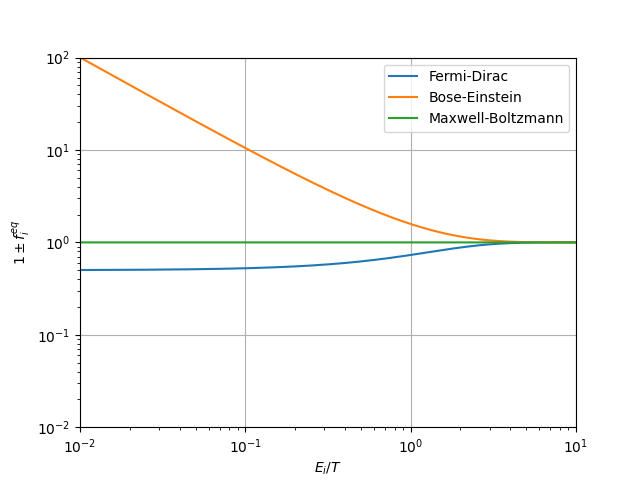
\includegraphics[width=0.7\linewidth]{graphs/1+-fi}
	\caption{Dependance of $1\pm f_i$ with $E_i/T$.}
	\label{fig:1-fi}
\end{figure}

For the process of annihilation ($1+2 \leftrightarrow 3+4$), where the particles $3$ and $4$ are in thermal equilibrium, and considering the conservation of energy ($E_1+E_2=E_3+E_4$) we check that
\begin{equation}
	f_3^{eq}f_4^{eq}=e^{-(E_3+E_4)/T}=e^{-(E_1+E_2)/T}=f_1^{eq}f_2^{eq}\,.
\end{equation}

The cross section for a process $1+2\rightarrow3+4$ is 
\begin{equation}
	\label{crosssection}
	\sigma=\frac{S_{12}S_{34}}{4\sqrt{(\mathcal{P}_1\cdot\mathcal{P}_2)^2-(m_1m_2)^2}}\int (2\pi)^4\delta^4(\mathcal{P}_1+\mathcal{P}_2-\mathcal{P}_3-\mathcal{P}_4)\frac{|M|^2}{g_1g_2}\frac{d\Pi_3d\Pi_4}{g_3g_4}\,.
\end{equation}

Using the \autoref{eqn:3.1}, for the number density as
\begin{equation}
	\label{dni}
	dn_i=\frac{g_i}{(2\pi)^3}\frac{d\vec{p}_i}{2E_i}\,,
\end{equation}
and the \autoref{crosssection}, we can simplify the \autoref{eqn:3.38} to
\begin{equation}
	\label{3.45}
	\int C[f_1] d\Pi_1 = -\int \sigma v_{\textrm{M{\o}ller}}\left[dn_1dn_2-dn_1^{eq}dn_2^{eq}\right]\,,
\end{equation}
where $v_{\textrm{M{\o}ller}}$, is the M{\o}ller velocity, and is defined as
\begin{equation}
	\label{vmoller}
	v_{\textrm{M{\o}ller}}=\frac{\sqrt{(\mathcal{P}_1\cdot\mathcal{P}_2)^2-(m_1m_2)^2}}{E_1E_2}\,,
\end{equation}
the M{\o}ller velocity turns the product $v_{\textrm{M{\o}ller}}n_1n_2$ invariant under Lorentz\,, \cite{GONDOLO}.

Therefore we can write our \autoref{3.45}, as
\begin{equation}
	\label{eqn:3.47}
	\frac{g_1}{(2\pi)^3}\int \frac{d\vec{p}_1}{2E_1}C[f_1]=-\langle\sigma v_{\textrm{M{\o}ller}}\rangle[n_1n_2-n_1^{eq}n_2^{eq}]\,,
\end{equation}
where the thermal averaged cross section is defined as
\begin{equation}
	\label{tacs}
	\langle \sigma v_{\textrm{M{\o}ller}}\rangle=\dfrac{\mathlarger{\int} (\sigma v_{\textrm{M{\o}ller}})dn_1^{eq}dn_2^{eq}}{\mathlarger{\int} dn_1^{eq}dn_2^{eq}}\,,
\end{equation}
for simplicity we are going to denote the thermal averaged cross-section as $\langle\sigma v\rangle$.

Let's take a look at the number density of the particles coupled with the thermal bath, knowing these particles will follow the Maxwell-Boltzmann distribution, with $\mu=0$, we can write the \autoref{eqn:3.17} as
\begin{equation}
	\label{nthermalbath}
	n=\frac{g}{(2\pi)^3}4\pi\int_{m}^{\infty} E\sqrt{E^2-m^2}e^{-E/T}dE\,,
\end{equation} 
where we use $E^2=|\vec{p}|^2+m^2$ and spherical symmetry of the momentum, $d\vec{p}=4\pi E \sqrt{E^2-m^2}dE$. The inferior limit comes from the minimum energy possible of the particle, which is its rest mass.

Integrating by parts the \autoref{nthermalbath}, we get
\begin{equation}
	n=\frac{g}{(2\pi)^3}4\pi\left(\frac{1}{3}\left[(E^2-m^2)^{3/2}e^{-E/T}\right]_m^\infty+\frac{1}{3T}\int_{m}^{\infty}(E^2-m^2)^{3/2}e^{-E/T}dE\right)\,,
\end{equation}
we can easily see that the left side gives zero, and the right side can be related to the Bessel function, which is defined as
\begin{equation}
	 \label{bessel}
	 K_\alpha(z)=\frac{\sqrt{\pi}}{\Gamma(\alpha+1/2)}\left(\frac{z}{2}\right)^\alpha\int_{1}^{\infty}(x^2-1)^{\alpha-1/2}e^{-zx}dx\,,
\end{equation}
and so making $x=E/m$ and $z=m/T$, and knowing that $\Gamma(5/2)=3\sqrt{\pi}/4$, we get
\begin{equation}
	\label{nbessel}
	n=\frac{g}{2\pi^2}m^2TK_2(m/T)\,.
\end{equation}

From Equations (\ref{tacs}) and (\ref{dni}) we can see that

\begin{equation}
	\label{eqn:3.52}
	\langle \sigma v_{\textrm{M{\o}ller}}\rangle=\dfrac{\mathlarger{\int}(\sigma v_{\textrm{M{\o}ller}})e^{-E_1/T}e^{-E_2/T}d^3p_1d^3p_2}{\mathlarger{\int} e^{-E_1/T}e^{-E_2/T}d^3p_1d^3p_2}	\,.
\end{equation}

Let's now consider that the particle 1 is equal to the particle 2, as it will be the main scope of this project.
Following the \autoref{nbessel}, it's easy to see that the denominator of the \autoref{eqn:3.52} will be
\begin{equation}
	\label{3.53}
	\int e^{-E_1/T}e^{-E_2/T}d\vec{p}_1d\vec{p}_2=(4\pi m^2 T K_2(m/T))^2\,,
\end{equation}
where $m=m_1=m_2$

Let's now look at the numerator of the \autoref{eqn:3.52}, using spherical symmetry ($d\vec{p}_i=4\pi E_i |\vec{p}_i| dE_i$) we can see that
\begin{equation}
	\label{volume1}
	d^3p_1d^3p_2=4\pi E_1 |\vec{p}_1| 4\pi E_2 |\vec{p}_2|  \frac{1}{2}dE_1dE_2d\cos(\theta)\,,
\end{equation}
where $\theta$ is the angle between $\vec{p}_1$ and $\vec{p}_2$, notice that the term $d\cos(\theta)/2$ is invariant under integration, for simplicity we are going to make a few changes of variables
\begin{equation}
	\left\{\begin{array}{l}
			E_+=E_1+E_2 \\
			E_-=E_1-E_2 \\
			s=2m^2+2E_1E_2-2|\vec{p}_1||\vec{p}_2|\cos(\theta)
	\end{array} \right.	\Leftrightarrow
	\left\{\begin{array}{l}
		E_1=\frac{E_++E_-}{2} \\
		E_2=\frac{E_+-E_-}{2} \\
		\cos(\theta)=\dfrac{-s+2m^2+2(E_+^2-E_-^2)}{2|\vec{p}_1||\vec{p}_2|}
	\end{array} \right.\,,
\end{equation}
where $s=\left(\mathcal{P}_1+\mathcal{P}_2\right)^2$ is a Mandelstam variable \cite{otto}.

Using the Jacobian matrix we can see that
\begin{align}
	\begin{array}{ll}
		dE_1dE_2d\cos(\theta)
		=&\left| 
		\begin{array}{lll} 
			\frac{\partial E_1}{\partial E_+} & \frac{\partial E_1}{\partial E_-} & \frac{\partial E_1}{\partial s}\\
			\frac{\partial E_2}{\partial E_+} & \frac{\partial E_2}{\partial E_-} & \frac{\partial E_2}{\partial s}\\
			\frac{\partial \cos(\theta)}{\partial E_+} & \frac{\partial \cos(\theta)}{\partial E_-} & \frac{\partial \cos(\theta)}{\partial s}
		\end{array} \right|dE_+dE_-ds \\ [15pt]
	&= (2|\vec{p}_1||\vec{p}_2|)^{-1}dE_+dE_-ds\,.
	\end{array}
\end{align}


The volume element, in \autoref{volume1} becomes

\begin{equation}
	\label{volume2}
	d^3p_1d^3p_2=2\pi^2E_1E_2dE_+dE_-ds\,,
\end{equation}
and the integration limits, from $E_1\geq m_1$, $E_2\geq m_2$, $|\cos(\theta)|\leq 1$, become
\begin{equation}
	\left\{
	\begin{array}{l}
		s \geq 4m^2 \\
		E_+\geq \sqrt{s} \\
		|E_-| \leq \sqrt{1-\frac{4m^2}{s}} \sqrt{E_+^2-s}
	\end{array}
	\right.\,.
\end{equation}

Therefore, the numerator from \autoref{eqn:3.52} will be

\begin{equation}
	\int (\sigma v_{\textrm{M{\o}ller}})e^{-E_1/T}e^{-E_2/T}d^3p_1d^3p_2=2\pi^2\int dE_- \int dE_+ \int \sigma v_{\textrm{M{\o}ller}} E_1 E_2 e^{-E_+/T}ds\,,
\end{equation}
then from the definition of $v_{\textrm{M{\o}ller}}$ in \autoref{vmoller},

\begin{align}
	\label{3.60}
	\begin{array}{ll}
		\mathlarger{\int} (\sigma v_{\textrm{M{\o}ller}})e^{-E_1/T}e^{-E_2/T}d^3p_1d^3p_2&=
		4\pi^2 \mathlarger{\int} \sigma G \sqrt{1-\frac{4m^2}{s}}ds \mathlarger{\int} e^{E_+/T}\sqrt{E_+^2-s}dE_+ \\ [15pt]
		&= 2\pi^2 T \mathlarger{\int} \sigma (s-4m^2) \sqrt{s}K_1(\sqrt{s}/T)ds\,,
	\end{array}
\end{align}
where we define $G \equiv v_{\textrm{M{\o}ller}}E_1E_2=\frac{1}{2}\sqrt{s(s-4m^2)}$ and we use the Bessel function, in \autoref{bessel}, with $\alpha=1$.

Let us use the Equations (\ref{3.53}) and (\ref{3.60}), to simplify the thermal averaged cross section, in \autoref{tacs}, to
\begin{equation}
	\label{sigmav}
	\langle \sigma v_{\textrm{M{\o}ller}}\rangle=\frac{1}{8m^4TK_2^2(m/T)}\int_{4m^2}^{\infty}\sigma(s-4m^2)\sqrt{s}K_1(\sqrt{s}/T)ds\,.
\end{equation}


%\chapter{Dark Matter candidate}
\label{chapter:candidate}

As discussed in \autoref{Chapter:introduction}, the key to find if a particle is a viable candidate for Dark Matter or not, is to check whether a particle is coupled or decoupled from the thermal bath, and calculate its abundance. 

In order to understand the thermal evolution of the universe, we need to compare the interaction rate, with the rate of expansion. 

The interactions of the particles occur within a homogeneous and isotropic gaseous equilibrium, we denominate this as the thermal bath. 
If the interactions are rapid enough to adjust to the changing of the temperature of the expanding universe, we can maintain our universe in a nearly thermal equilibrium.
The particles that remain in equilibrium with the thermal bath are denominated as being coupled with the thermal bath, and the ones that leave the equilibrium, are decoupled from the thermal bath.

We can say that a particle is either coupled or decoupled with the thermal bath, by the relation between the rate of interaction of said particle, $\Gamma$, and the rate of expansion of the universe, $H$
\begin{align}
	\label{eq}
	\begin{array}{ll}
		\Gamma > H \quad (coupled) \\
		\Gamma < H \quad (decoupled)
	\end{array}
\end{align}


\section{Interaction rate}

In this section, we are going to check if the pseudo-Goldstone boson studied in \autoref{chapter:Ultralight Bosons} is a viable candidate for DM.

The rate of interaction is given by
\begin{equation}
	\Gamma = n\langle \sigma v \rangle\,,
\end{equation}
where $n$ is the number density of our particle.

For the rate of interaction of pNGB we are only interested in the processes of annihilation $\theta+\theta \rightarrow SM + SM$, which were our main focus in Section \autoref{chapter:thermodynamicsofearlyuniverse}.
And so the rate of interaction is 
\begin{equation}
	\Gamma=\frac{g}{16m^2\pi^2K_2(m/T)}\int_{4m^2}^\infty\sigma(s-4m^2)\sqrt{s}K_1\left(\frac{\sqrt{s}}{T}\right)ds\,.
\end{equation}

To calculate the rate of interaction, we need to determine the cross-section of the reaction, $\sigma$ in \autoref{sigmav}, where the squared amplitude of the process, $|\mathcal{M}|^2$ in \autoref{crosssection}, was calculated using CalcHEP.

CalcHEP is a package for the calculation of Feynman diagrams \cite{Belyaev_2013}, implementing the model studied in the Section \autoref{chapter:Ultralight Bosons}, considering only the $s$-channels with mediators like the Higgs and $h_2$, where the $t$ and $u$ channels were not considered as they would have near to no impact on the amplitude of the process of annihilation of pGB.
And then for the calculation of the integrals, we used Cuba, a library for multidimensional numerical integration \cite{HAHN200578}, in C++ language.



For simplification reasons, we are going to make all the coupling terms, $\lambda_{H}$, $\lambda_{H\phi}$ and $\lambda_{\phi}$ constant which are bounded by the conditions in Eq.(\ref{couplingtermconditions}) and vary the VEV, $v_\sigma$, which is directly related to the mass of the Higgs.
If we recall the \autoref{masses}, we can manipulate both $h_1$ and $h_2$ masses, in order for one of them to equal the mass of the SM-Higgs and the other to have any values depending on $v_\sigma$.
And so we obtain the following rates of interaction 


\begin{figure}[H]
	\centering
	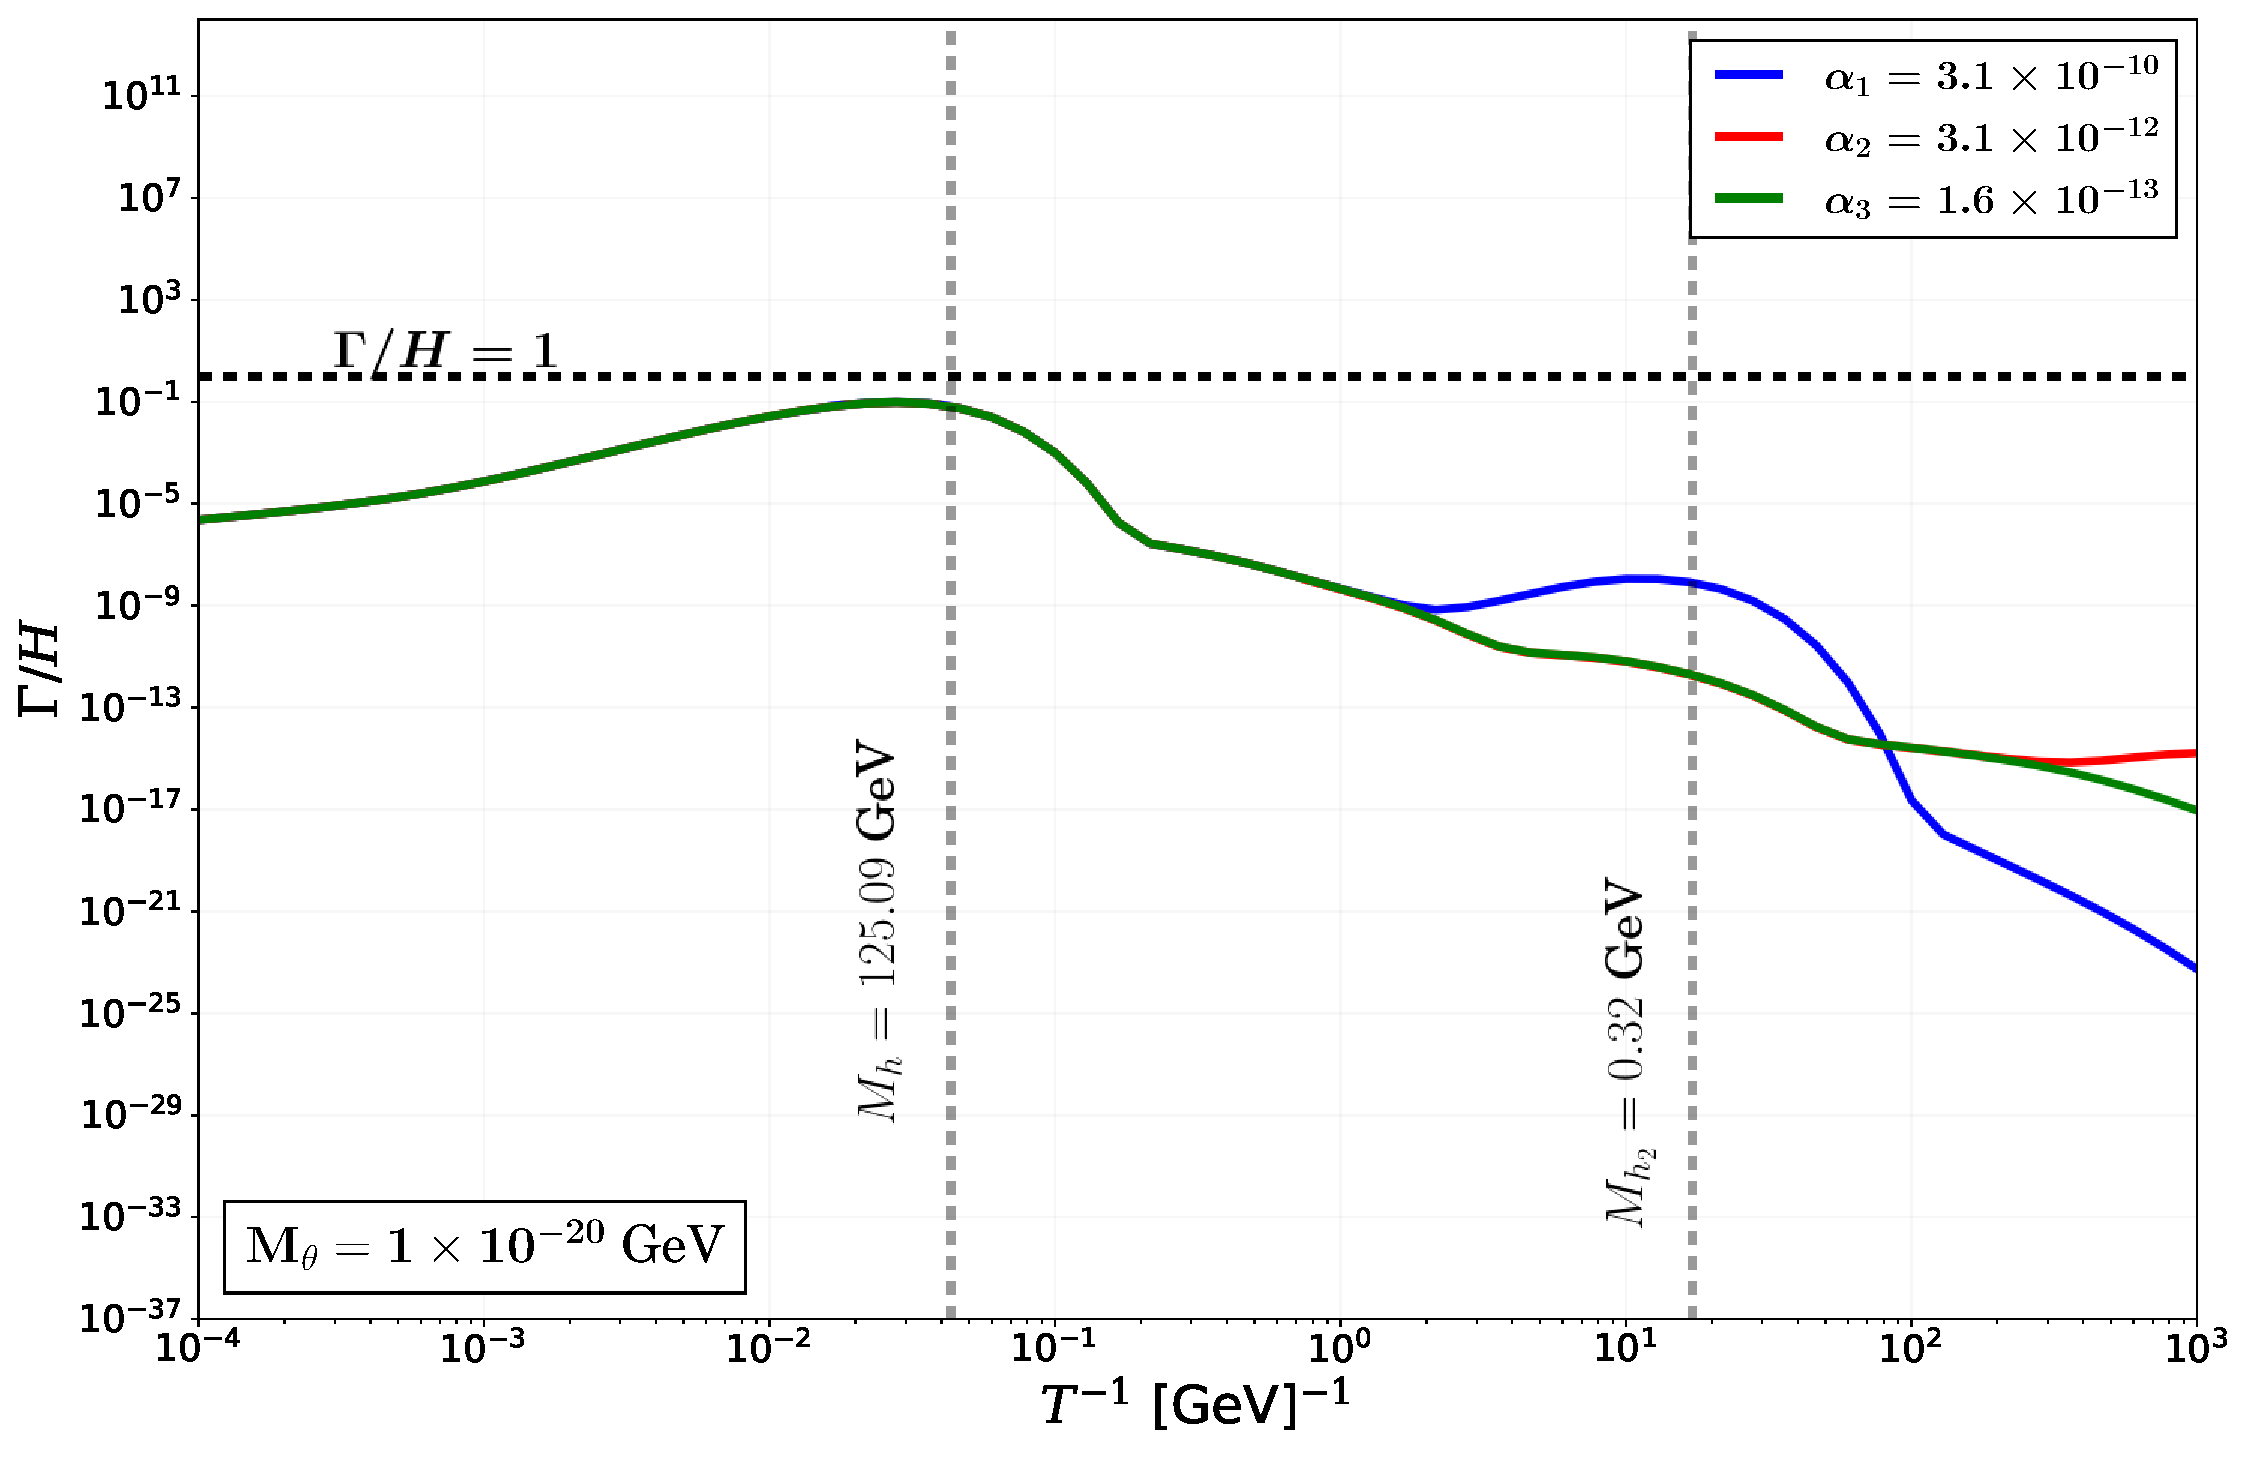
\includegraphics[width=0.7\linewidth]{graphs/ratedm_lesser}
	\caption{Rate of interaction divided by Hubble assuming $m_h \gg m_{h_2}$, for $\nu_\sigma=1$ \si{G\eV} ($M_{h_2} = 3.2\times10^{-1}$ \si{G\eV}),  $\nu_\sigma=0.01$ \si{G\eV} ($M_{h_2} = 3.2\times10^{-3}$ \si{G\eV}) and  $\nu_\sigma= 5\times10^{-4}$ \si{G\eV} ($M_{h_2} = 1.6\times10^{-4}$ \si{G\eV}), for blue, green and red curves, respectively.  Additionally, we have used $\lambda_H\sim0.26$, $\lambda_{H\phi}=2\times10^{-8}$ and $\lambda_\phi=0.1$\,.}
	\label{fig:ratelesser}
\end{figure}

\begin{figure}[H]
	\centering
	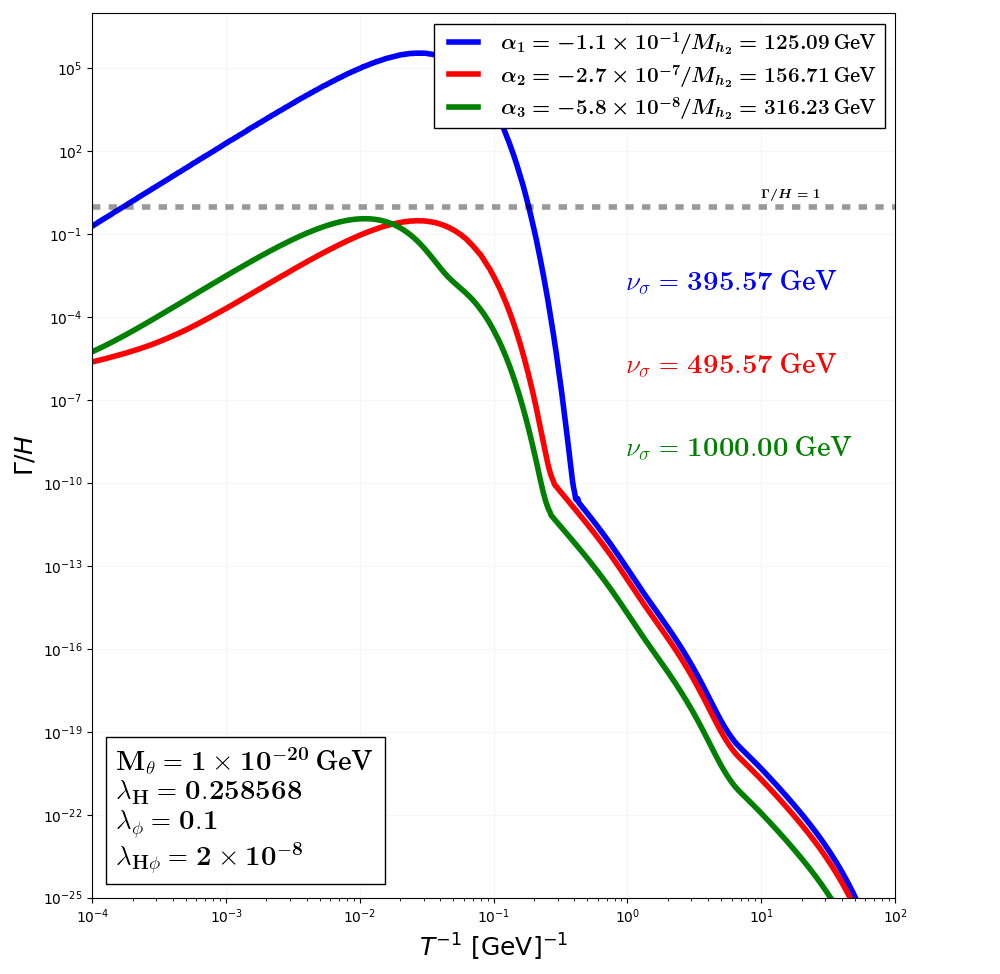
\includegraphics[width=0.75\linewidth]{graphs/ratedm_equal}
	\caption{Rate of interaction divided by Hubble assuming $m_h = m_{h_2}$, for $\nu_\sigma=395.57$ \si{G\eV} ($M_{h_2}=125.09$ \si{G\eV}),  $\nu_\sigma=495.57$ \si{G\eV} ($M_{h_2}=156.71$ \si{G\eV}) and  $\nu_\sigma=10^3$ \si{G\eV}  ($M_{h_2}=316.23$ \si{G\eV}), for blue, green and red curves, respectively.  Additionally, we have used $\lambda_H\sim0.26$, $\lambda_{H\phi}=2\times10^{-8}$ and $\lambda_\phi=0.1$\,.}
	\label{fig:rateequal}
\end{figure}

\begin{figure}[H]
	\centering
	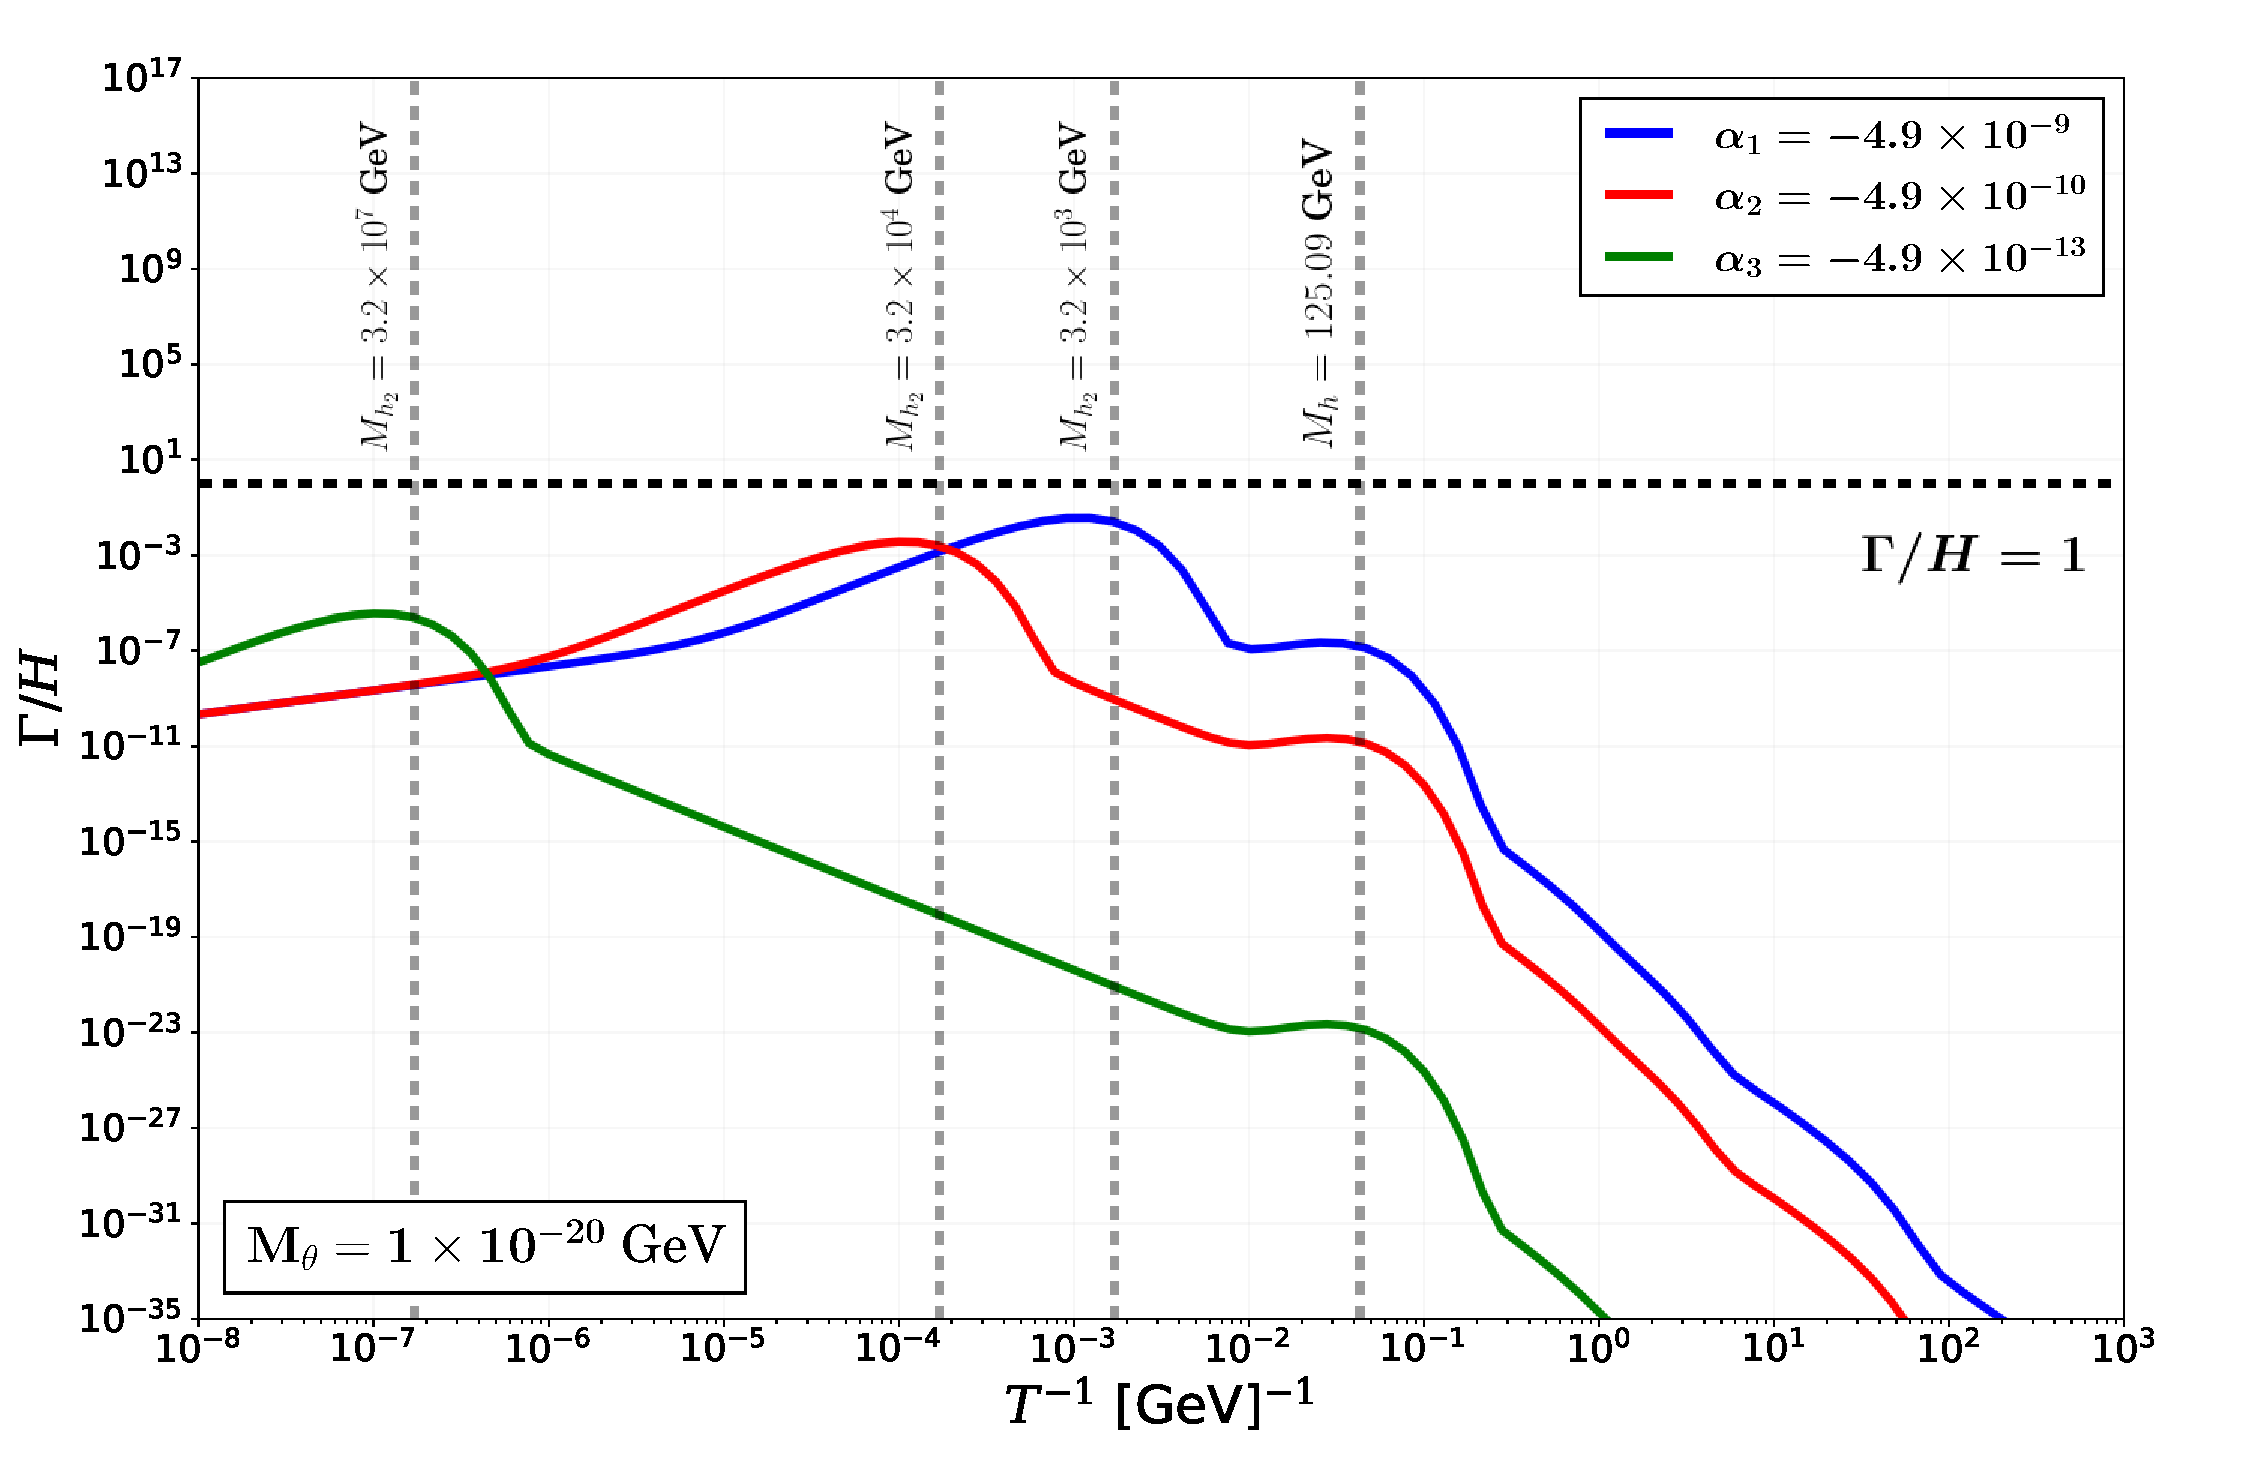
\includegraphics[width=0.8\linewidth]{graphs/ratedm_greater}
	\caption{Rate of interaction divided by Hubble assuming $m_h \ll m_{h_2}$, for $\nu_\sigma=10^4$ \si{G\eV} ($M_{h_2} = 3.2\times10^{3}$ \si{G\eV}),  $\nu_\sigma=10^5$ \si{G\eV} ($M_{h_2} = 3.2\times10^{4}$ \si{G\eV}) and  $\nu_\sigma= 10^8$ \si{G\eV} ($M_{h_2} = 3.2\times10^{7}$ \si{G\eV}), for blue, green and red curves, respectively.  Additionally, we have used $\lambda_H\sim0.26$, $\lambda_{H\phi}=2\times10^{-8}$ and $\lambda_\phi=0.1$\,.}
	\label{fig:rategreater}
\end{figure}

We can prove that as long as, the mixing angle, $\alpha\lesssim10^{-7}$, our pNGB doesn't couple with the thermal bath, and so doesn't become relativistic (cold). Notice that this constraint in the mixing angle, allows our VEV $v_\sigma$ to become a free parameter, as long as the quartic coupling terms remain the same. As mentioned in \autoref{chapter:Ultralight Bosons}, the mixing angle being small only allows decays of the $h_2$ into $\theta\theta$, and seeing as $v_\sigma$ becomes a free parameter, for large values of $v_\sigma$, this decay also disappears.

Note that there is a resonance whenever the temperature is approximately equal to the mass of the mediator, SM-Higgs or $h_2$, for $T\thicksim m_{h_{1,2}}/5.4$\cite{kolb}.

\section{Misalignment}
 
In this section, we are going to consider that the soft-symmetry breaking of the U$(1)_G$ symmetry, which produced the pNGB, occurred before the end of inflation. Inflation is a theory that explains the exponential rate of expansion of the early universe.

The temperature at which inflation occurred is bounded by the 

Using the \autoref{newvsoft}, and introducing the misalignment angle as $\Theta = \dfrac{2\theta}{v_\sigma}$
\begin{equation}
    V_{\textrm{soft}}(\Theta)\simeq \frac{m_\theta^2}{2}\left(\frac{v_\sigma}{2}\right)^2\Theta^2\,.
\end{equation}

Using the energy-momentum tensor, $T^{\mu}_\nu$, of $\theta$ 
\begin{equation}
    T^\mu_\nu=g^{\mu\alpha}(\partial_\alpha\theta)(\partial_\nu\theta)-\frac{\delta^\mu_\nu}{2}[g^{\alpha\beta}(\partial_\alpha\theta)(\partial_\beta\theta)+2V(\theta)]\,,
\end{equation}
where $g^{\mu\nu}=diag(-1,1,1,1)$ and the energy density reads as \cite{Marsh_2016}\cite{kolb}
\begin{align}
\label{densityenergy}
\begin{array}{ccc}
    &\rho_\theta=-T^0_0=-g^{0\alpha}(\partial_\alpha\theta)(\partial_0\theta)+\dfrac{1}{2}[g^{\alpha\beta}(\partial_\alpha\theta)(\partial_\beta\theta)+2V(\theta)]=\dfrac{1}{2}\left(\dfrac{\partial\theta}{\partial t}\right)^2-\dfrac{1}{2}\dfrac{\vec{\nabla}^2\theta}{a^2}+V(\theta)=\\ [5pt]
    &=\dfrac{1}{2}\left(\dfrac{\partial\theta}{\partial t}\right)^2+V(\theta)=\left(\dfrac{v_\sigma}{2}\right)^2\left[\dfrac{\dot{\Theta}^2}{2}+\dfrac{m_\theta^2}{2}\Theta^2\right]\,,
\end{array}
\end{align}
where $\theta$ only varies with time and is the same in the universe.

Knowing that the energy density of $\theta$ can be given by
\begin{equation}
\label{rhoa}
    \rho_\theta(a)=\rho_\theta(a_i)\left(\dfrac{a_i}{a}\right)^3\,,
\end{equation}
where $a$ is the scale factor, and the $a_i$ relates do any value of the scale factor.

In the radiation era of the universe, we have that, $a\propto \sqrt{t}$, where $t$ is the age of the universe.

The equation of motion for $\theta$ can be obtained varying the action, $S=\int \mathcal{L} a^3 d^4x$ , where $a$
is the scale factor, and computing the D’Alembertian for the Friedmann–Robertson–Walker (FRW) metric we obtain\cite{Marsh_2016}
\begin{equation}
\label{motion}
    \ddot{\Theta}^2+3H\dot{\Theta}+m_\theta^2\Theta=0\,.
\end{equation}

\begin{figure}[H]
	\centering
	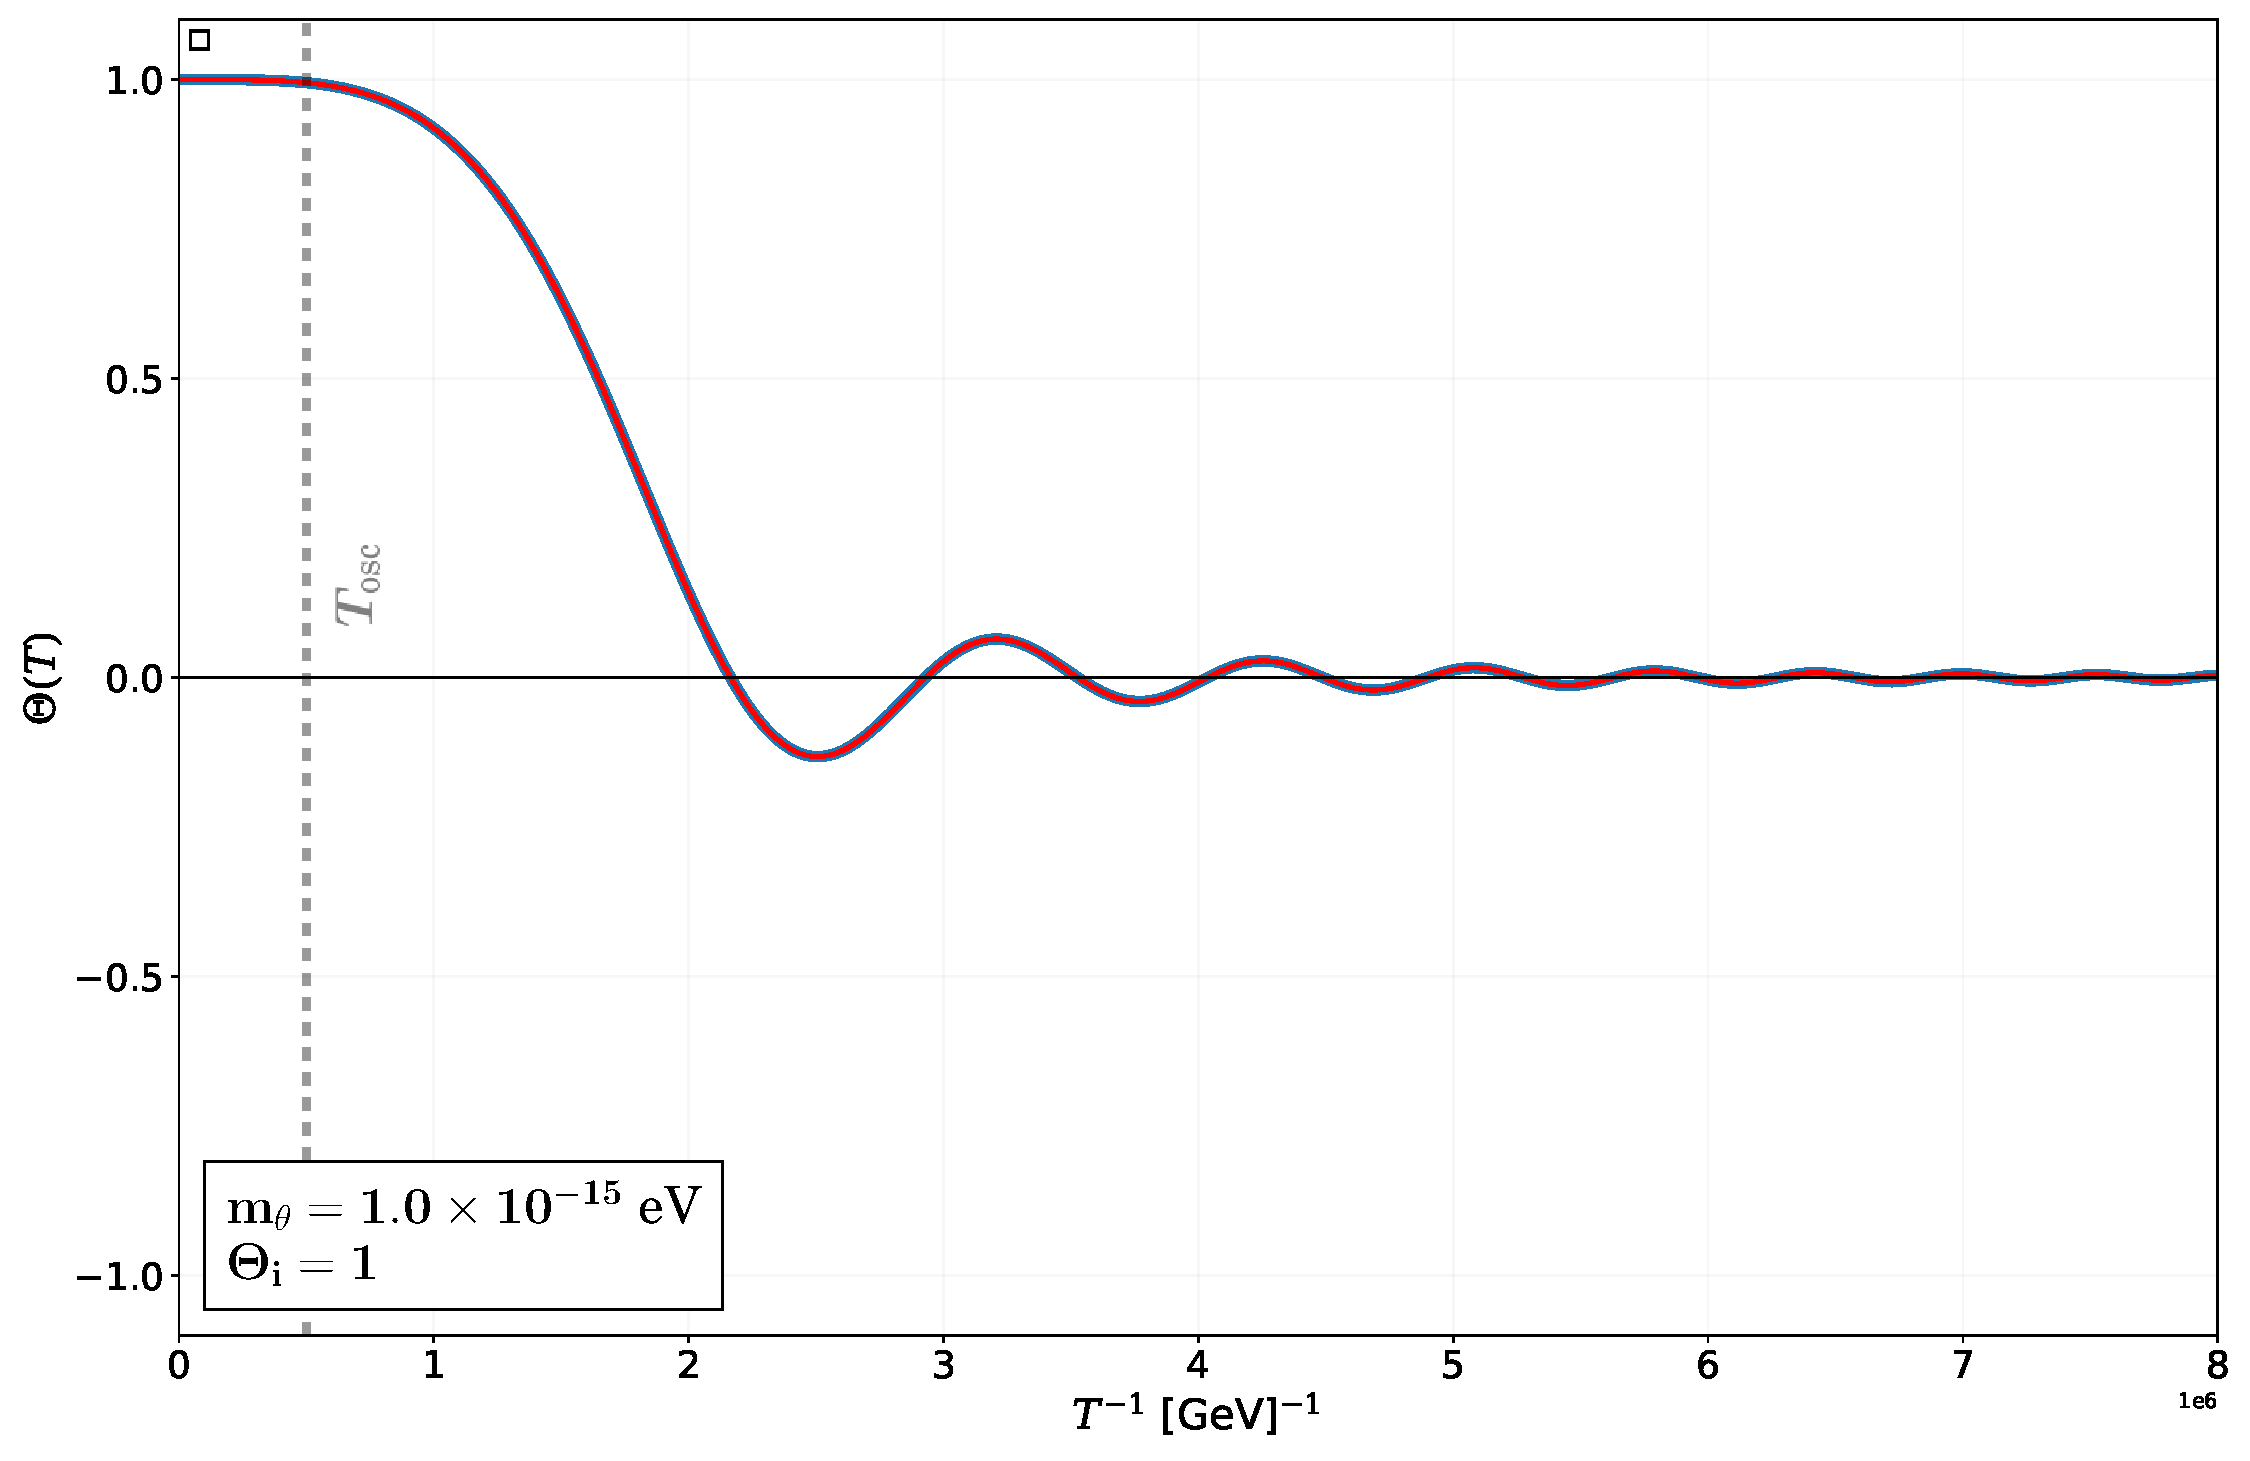
\includegraphics[width=0.9\linewidth]{graphs/motion.pdf}
	\caption{Solution of the equation of motion in \autoref{motion}\,.}
	\label{fig:motion}
\end{figure}

The \autoref{fig:motion}, allows us to see that the misalignment angle, $\Theta$, is constant for $T^{-1}\in[0,T^{-1}_{\textrm{osc}}]$, and so we can say from \autoref{densityenergy} that
\begin{equation}
    \rho_\theta(a_\textrm{osc})=\left(\dfrac{v_\sigma}{2}\right)^2\dfrac{m_\theta^2}{2}\Theta_\textrm{osc}^2\,.
\end{equation}

Using the \autoref{rhoa}, for an $a_i=a_\textrm{osc}$, we have
\begin{equation}
\label{rhoaa}
    \rho_\theta(a)=\left(\dfrac{v_\sigma}{2}\right)^2\dfrac{m_\theta^2}{2}\Theta_\textrm{osc}^2\left(\dfrac{a_\textrm{osc}}{a}\right)^3\,.
\end{equation}

Let us take a look at the entropy in the primordial universe, it can be written in terms of the pressure, $P$, and density of energy, $\rho$, as
\begin{equation}
    S=sa^3=\dfrac{\rho+P}{T}a^3\,,
\end{equation}
where $s$ is entropy density, recalling Equations (\ref{3.32}) and (\ref{eqn:3.16}) we have that the entropy can be written as
\begin{equation}
    S=\dfrac{2\pi^2}{45}g_{*s}(T)T^3a^3\,,
\end{equation}
where, $g_{*s}(T)$ is
\begin{equation}
	g_{*s}(T)=\sum\limits_{b}g_b\left(\frac{T_b}{T}\right)^3+\dfrac{7}{8}\sum\limits_{f}g_f\left(\frac{T_f}{T}\right)^3\,.
\end{equation}

Taking the following ratio,
\begin{equation}
\label{ratioS}
    \dfrac{S_\textrm{osc}}{S}=\dfrac{g_{*s}(T_\textrm{osc})}{g_{*s}(T)}\left(\dfrac{T_\textrm{osc}a_\textrm{osc}}{Ta}\right)^3\,,
\end{equation}
knowing that in the primordial universe the entropy is constant, so $S_\textrm{osc}=S$, the \autoref{ratioS} gets turned into
\begin{equation}
\label{aosc/a}
       \left(\dfrac{a_\textrm{osc}}{a}\right)^3=\dfrac{g_{*s}(T)}{g_{*s}(T_\textrm{osc})}\left(\dfrac{T}{T_\textrm{osc}}\right)^3\,.
\end{equation}

Using the \autoref{aosc/a}, the current energy density of $\theta$, in \autoref{rhoaa}, becomes
\begin{equation}
    \label{rhoaaa}
    \rho_\theta(a_0)=\left(\dfrac{v_\sigma}{2}\right)^2\dfrac{m_\theta^2}{2}\Theta_\textrm{osc}^2\dfrac{g_{*s}(T_0)}{g_{*s}(T_\textrm{osc})}\left(\dfrac{T_0}{T_\textrm{osc}}\right)^3\,.
\end{equation}
 
The current relic density of any matter is given by
\begin{equation}
    \Omega^0=\dfrac{\rho(a_0)}{\rho_\textrm{crit}}\,,
\end{equation}
and so using \autoref{rhoaaa}, the current relic density of $\theta$ reads as
\begin{equation}
    \Omega^0_\theta=\dfrac{\rho_\theta(a_0)}{\rho_\textrm{crit}}=\frac{1}{\rho_\textrm{crit}}\left(\dfrac{v_\sigma}{2}\right)^2\dfrac{m_\theta^2}{2}\Theta_\textrm{osc}^2\dfrac{g_{*s}(T_0)}{g_{*s}(T_\textrm{osc})}\left(\dfrac{T_0}{T_\textrm{osc}}\right)^3\,.
\end{equation}

This can be further simplified as we know most of this terms,  $\rho_\textrm{crit}=1.88\times 10^{-29}h^2 \si{\g\cm^{-3}}=8.1\times10^{-47}h^2$ \si{G\eV^4}, using the \autoref{masses} for $\mu_s^2=-m_\theta^2/2$, $g_{*s}(T_0)=3.91$, $g_*(T_0)=3.36$ and $T_0=2.3\times10^{-4}$ \si{\eV}, and finally we have that the current relic density of $\theta$ is
\begin{equation}
    \Omega^0_\theta h^2=0.11\left(\dfrac{m_\theta}{10^{-14}\si{\eV}}\right)^{1/2}\left(\dfrac{v_\sigma}{\sqrt{50}\times10^{17}\si{G\eV}}\right)^{2}\left(\dfrac{\Theta_\textrm{osc}}{10^{-3}}\right)^{2}\left(\dfrac{3.91}{g_{*s}(T_\textrm{osc})}\right)\left(\dfrac{g_*(T_\textrm{osc})}{3.36}\right)^{3/4}\,.
\end{equation}
 
\begin{figure}[H]
	\centering
	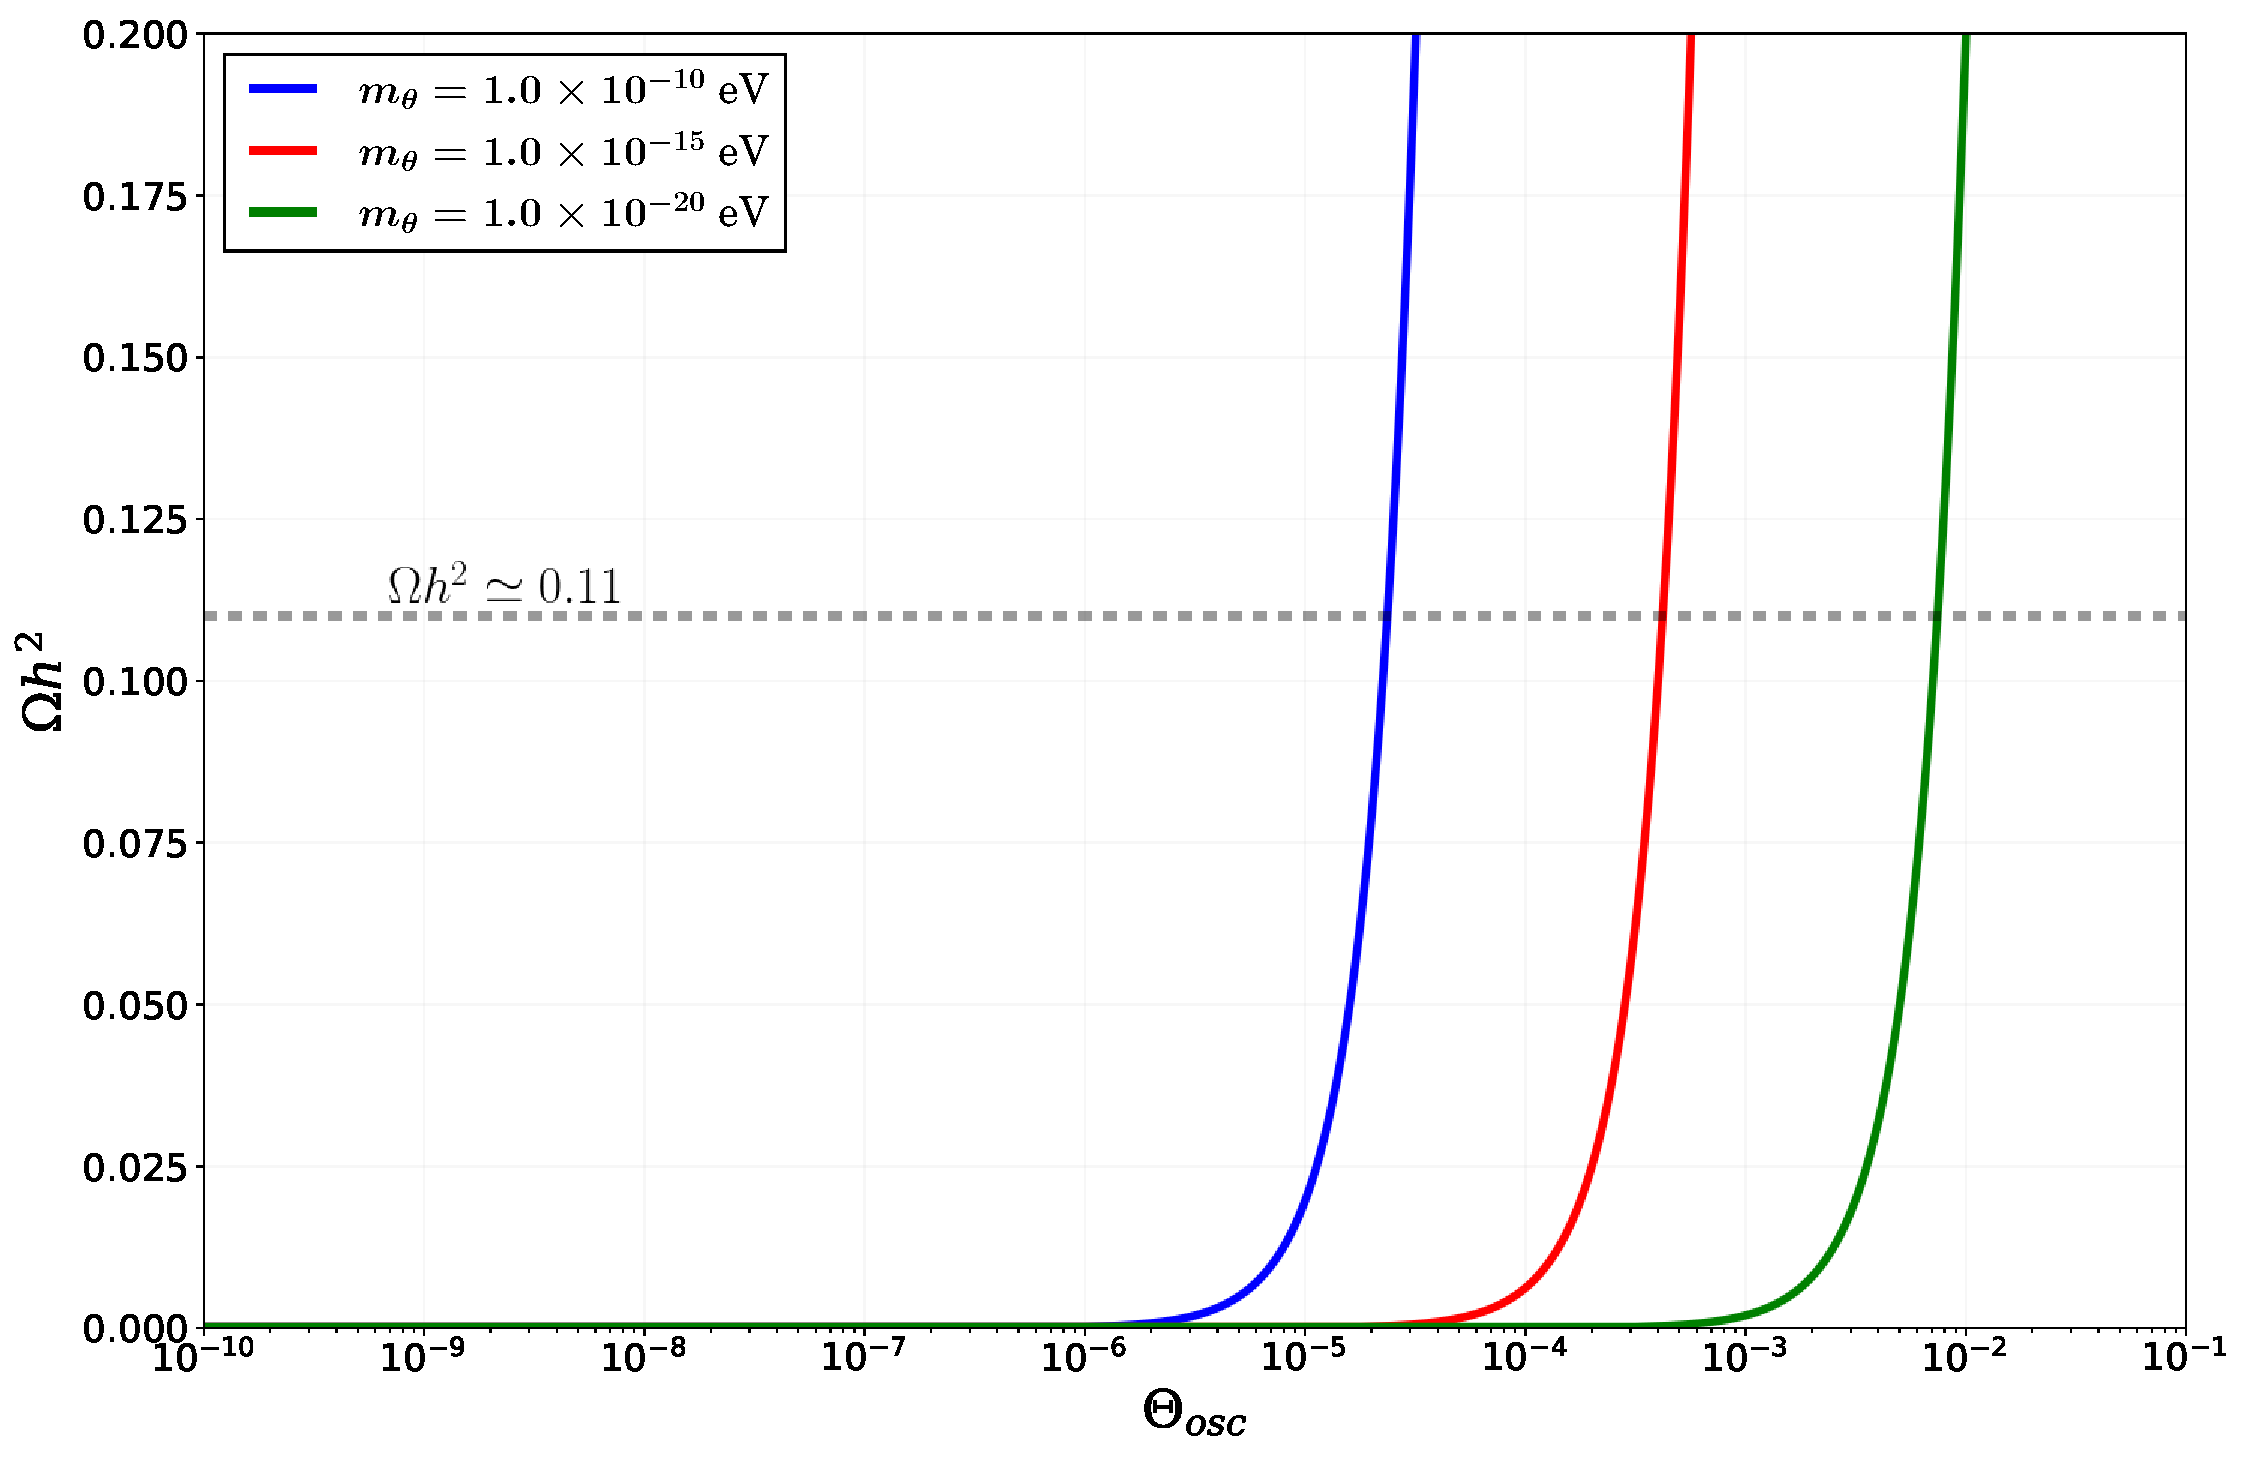
\includegraphics[width=0.9\linewidth]{graphs/relic_density.pdf}
	\caption{Relic density variating $\Theta_i$, with $v_\sigma=3\times 10^{18}$, for various values of $m_\theta$\,.}
	\label{fig:relicdesity}
\end{figure}

The \autoref{fig:relicdesity} allows us to determine the required initial misalignment angle, $\Theta_\textrm{osc}$, for certain mass and $v_\sigma$.



% End of Thesis text ---------------------------------------------------------
% Including files is advised:


%Appendix


%Print all used references

\begingroup
\renewcommand{\bibfont}{\footnotesize}

%Redefine References name
\defbibheading{bibliography}[References]{
	\chapter{#1}
}
\SingleSpacing
\setlength\bibitemsep{8pt}
\printbibliography[heading=bibliography]
\endgroup

%Load appendix
%\include{appendix-a}


\end{document}
